\documentclass[10pt,a4paper]{ctexart}

\input{TeXStyle/preamble}

\begin{document}
%%%%%%封面页
\input{TeXStyle/cover}

%%%%%%目录
\newpage
\pagenumbering{Roman}
\setcounter{page}{1}
\tableofcontents

\ctexset{section = {
        format=\zihao{4}\bfseries
    },
    subsection = {
        format={\zihao{-4}\bfseries}
    }
}

%%%%%%正文
\newpage
\pagenumbering{arabic}
\setcounter{page}{1}

\section{实验目的}
\begin{enumerate}[nosep,label={(\arabic*)}]
\item 通过编程实现高精度惯导数据处理,加深对惯性导航原理及机械编排算法的理解;
\item 通过分析纯惯导解算位置,速度和姿态的误差,对惯性导航的误差累积形成直观认识;
\item 初步掌握零速修正(将速度重置为零),分析和理解零速修正对惯性导航误差的修正作用.
\end{enumerate}

\section{实验原理}
公式的推导部分在\href{run:./Alogrithm/INS.pdf}{\textsl{另一篇文档(INS.pdf)}},本实验报告只写出编程使用到的公式.
\subsection{欧拉角与四元数}
我们用一组欧拉角描述载体的姿态,包括航向角$\psi$,俯仰角$\theta$,横滚角$\phi$,那么$b$系到$n$系的旋转矩阵为
\[
    \mathbf{C}_b^n = \begin{bmatrix}
        \cos \theta \cos \psi & - \cos \phi \sin \psi + \sin \phi \sin \theta \cos \psi & \sin \phi \sin \psi + \cos \phi \sin \theta \cos \psi   \\
        \cos \theta \sin \psi & \cos \phi \cos \psi + \sin \phi \sin \theta \sin \psi   & - \sin \phi \cos \psi + \cos \phi \sin \theta \sin \psi \\
        - \sin \theta         & \sin \phi \cos \theta                                   & \cos \phi \cos \theta
    \end{bmatrix},
\]
显然,根据旋转矩阵,可以反推出欧拉角为
\begin{align*}
    \phi   & = \arctan \frac{c_{32}}{c_{33}}, \\
    \theta & = - \arcsin c_{31},              \\
    \psi   & = \arctan \frac{c_{21}}{c_{11}}.
\end{align*}
其中$\arctan$均为\code{C\#}中的\code{Math.Atan2}函数.欧拉角也可以转换为对应的四元数:
\[
    q_b^n = \begin{bmatrix}
        \cos \dfrac{ \phi }{2}\cos \dfrac{ \theta }{2}\cos \dfrac{ \psi }{2} + \sin \dfrac{ \phi }{2}\sin \dfrac{ \theta }{2}\sin \dfrac{ \psi }{2}     \\[7pt]
        \sin \dfrac{ \phi }{2}\cos \dfrac{ \theta }{2}\cos \dfrac{ \psi }{ 2} - \cos \dfrac{ \phi }{ 2}\sin \dfrac{ \theta }{ 2}\sin \dfrac{ \psi }{ 2} \\[7pt]
        \cos \dfrac{ \phi }{ 2}\sin \dfrac{ \theta }{ 2}\cos \dfrac{ \psi }{ 2} + \sin \dfrac{ \phi }{ 2}\cos \dfrac{ \theta }{ 2}\sin \dfrac{ \psi }{ 2} \\[7pt]
        \cos \dfrac{ \phi }{ 2}\cos \dfrac{ \theta }{ 2}\sin \dfrac{ \psi }{ 2} - \sin \dfrac{ \phi }{ 2}\sin \dfrac{ \theta }{ 2}\cos \dfrac{ \psi }{ 2}
    \end{bmatrix}.
\]
反过来,四元数
\[
    q_b^n =(q_0,q_1,q_2,q_3)
\]
可以转换为旋转矩阵
\[
    \mathbf{C}_b^n = \begin{bmatrix}
    q_0^2 + q_1^2 - q_2^2 - q_3^2 & 2(q_1q_2 - q_0q_3) & 2(q_1q_3 + q_0q_2) \\
    2(q_1q_2 + q_0q_3) & q_0^2 - q_1^2 + q_2^2 - q_3^2 & 2(q_2q_3 - q_0q_1) \\
    2(q_1q_3 - q_0q_2) & 2(q_2q_3 + q_0q_1) & q_0^2 - q_1^2 - q_2^2 + q_3^2 
    \end{bmatrix}.
\]
等效旋转矢量只是单位四元数的不同表达形式,记单位四元数$q=\cos \theta +u\sin\theta$,如果三维向量$\phi$的方向与$u$的方向相同,模长等于$2\theta$,那么我们称$\phi$是等效旋转矢量.显然有
\begin{equation}\label{eq:rotationVecToQuaternion}
    q = \cos \frac{\theta}{2}  + \frac{ \phi }{|\phi|} \sin\frac{ |\phi| }{2}.
\end{equation}

\subsection{惯性导航算法}\label{sec:INS}

记陀螺仪在$t_k$时刻的角增量输出为$\Delta\boldsymbol{\theta}_k$,速度增量输出为$\Delta\boldsymbol{v}_k$, IMU在$t_k$时刻的姿态用四元数$q_{b(k)}^{n(k)}$表示,速度为$\boldsymbol{v}_k$(用NED表示),经纬高分别为$\lambda_k,\varphi_k,h_k$.
\subsubsection*{姿态算法}
首先用等效旋转矢量更新$b$系,即
\begin{gather*}
    \boldsymbol{\phi}_k =\Delta\boldsymbol{\theta}_k + \frac{1}{12}\Delta\boldsymbol{ \theta }_{k - 1} \times \Delta\boldsymbol{\theta}_k,\\
    \boldsymbol{q}_{b(k)}^{b(k - 1)} =\frac{\cos |\boldsymbol{\phi}_k|}{2} + \frac{ \sin | \boldsymbol{\phi}_k |}{2} \frac{\boldsymbol{\phi}_k}{| \boldsymbol{\phi}_k |}.
\end{gather*}
再用等效旋转矢量更新$n$系,即
\begin{gather*}
    \boldsymbol{\zeta}_k =[\boldsymbol{\omega}_{ie}^n(t_{k - 1}) +\boldsymbol{\omega}_{en}^n(t_{k - 1})]\Delta t,\\
    \boldsymbol{q}_{n(k - 1)}^{n(k)} =\frac{\cos |\boldsymbol{\zeta}_k|}{2} + \frac{ \sin | \boldsymbol{\zeta}_k |}{2} \frac{\boldsymbol{\zeta}_k}{| \boldsymbol{\zeta}_k |}.
\end{gather*}
最后计算当前时刻的四元数:
\[
    \boldsymbol{q}_{b(k)}^{n(k)} = \boldsymbol{q}_{n(k - 1)}^{n(k)}\boldsymbol{q}_{b(k - 1)}^{n(k - 1)}\boldsymbol{q}_{b(k)}^{b(k - 1)}.
\]
为避免计算误差累积,所以需要对$\boldsymbol{q}_{b(k)}^{n(k)}$作单位化处理.

\subsubsection*{速度更新算法}

计算比力积分项:
\begin{gather*}
    \Delta\boldsymbol{v}_{f,k}^{b(k - 1)} =\Delta\boldsymbol{v}_k + \frac{1}{2}\Delta\boldsymbol{\theta}_k\times\Delta\boldsymbol{v}_k + \frac{1}{12}(\Delta\boldsymbol{\theta}_{k - 1}\times\Delta\boldsymbol{v}_k +\Delta\boldsymbol{v}_{k - 1}\times\Delta\boldsymbol{\theta}_{k}),\\
    \boldsymbol{\zeta}_{n(k - 1),n(k)} =(\boldsymbol{\omega}_{ie}^n +\boldsymbol{\omega}_{en}^n)_{k - \frac{1}{2}}(t_k - t_{k - 1}),\\
    \Delta\boldsymbol{v}_{f,k}^n = \left[\mathbf{I} - \frac{1}{2}(\boldsymbol{\zeta}_{n(k - 1),n(k)}\times)\right]\mathbf{C}_{b(k - 1)}^{n(k - 1)}\Delta\boldsymbol{v}_{f,k}^{b(k - 1)}.
\end{gather*}
计算重力和哥氏积分项:
\[
    \Delta\boldsymbol{v}_{g /cor,k}^n =[\boldsymbol{g}_p^n -(2\boldsymbol{\omega}_{ie}^n +\boldsymbol{\omega}_{en}^n)\times\boldsymbol{v}^n]_{k - \frac{1}{2}}(t_k - t_{k - 1}).
\]
计算当前时刻的速度:
\[
    \boldsymbol{v}_k =\boldsymbol{v}_{k - 1} +\Delta\boldsymbol{v}_{f,k}^n +\Delta\boldsymbol{v}_{g /cor,k}^n.
\]

\subsubsection*{位置更新算法}
由于位置更新需要用到当前时刻的速度,所以位置更新应在速度更新之后.高程更新:
\[
    h_k = h_{k - 1} - \frac{1}{2}(v_{D,k - 1} + v_{D,k})(t_k - t_{k - 1}).
\]
纬度更新:
\[
    \varphi_k =\varphi_{k - 1} + \frac{v_{N,k} + v_{N,k - 1}}{2(R_{M,k - 1} +\overline{h})}(t_k - t_{k - 1}). 
\]
经度更新:
\[
    \lambda_k =\lambda_{k - 1} + \frac{v_{E,k} + v_{E,k - 1}}{2(R_{N,k - \frac{1}{2}} +\overline{h})\cos \overline{\varphi}}(t_k - t_{k - 1}). 
\]
其中
\[
    \overline{h} = \frac{h_k + h_{k - 1}}{2},\overline{\varphi} = \frac{\varphi_k +\varphi_{k - 1}}{2} .
\]

\section{实验内容}

实验流程如图\ref{fig:Flowchart}所示.
\begin{figure}[htbp]
\centering
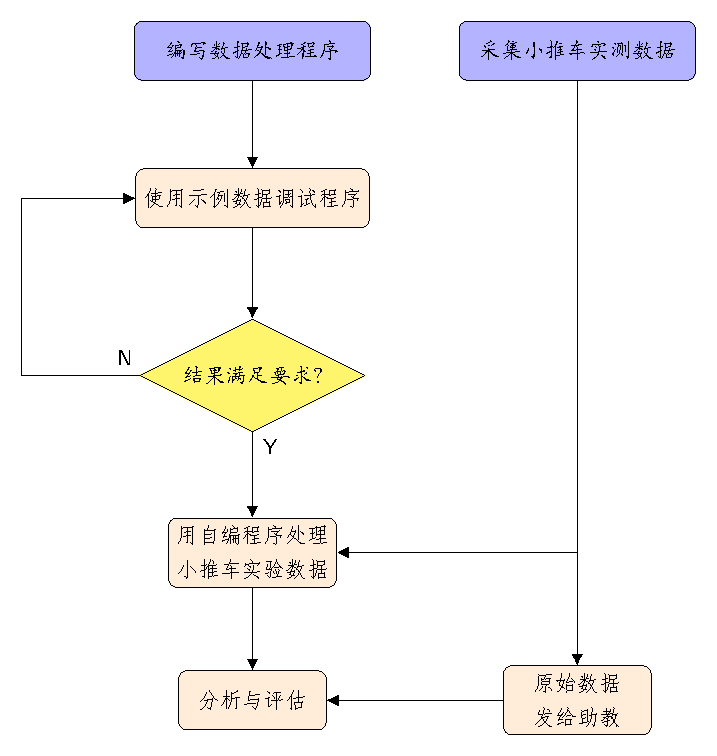
\includegraphics[scale=0.95]{Figures/Flowchart.pdf}
\caption{实验流程}
\label{fig:Flowchart}
\end{figure}

\subsection{用示例数据验证纯惯导程序}\label{subsec:3.1}
示例数据是用典型导航级惯导在车载测试场景下采集的原始IMU数据,参照结果由课程组经纯惯导解算得到.
\begin{table}[htbp]
\centering
    \begin{tblr}{colspec={cccccc},hline{1,3,Z} = {1pt}}
        \SetCell[c=6]{c} IMU原始数据({\ttfamily IMU.bin}) & & & & & \\
        序号 & 数据 & 单位 & 类型 & 字节数 & 备注 \\ 
        1 & {\ttfamily time} & s & {\ttfamily double} & 8 & 时间 \\
        2 & {\ttfamily gyro[0]} & rad & {\ttfamily double} & 8 & {\sffamily X}轴陀螺数据(角增量) \\
        3 & {\ttfamily gyro[1]} & rad & {\ttfamily double} & 8 & {\sffamily Y}轴陀螺数据(角增量) \\
        4 & {\ttfamily gyro[2]} & rad & {\ttfamily double} & 8 & {\sffamily Z}轴陀螺数据(角增量) \\
        5 & {\ttfamily acc[0]} & m/s & {\ttfamily double} & 8 & {\sffamily X}轴加速度计数据(速度增量) \\
        6 & {\ttfamily acc[1]} & m/s & {\ttfamily double} & 8 & {\sffamily Y}轴加速度计数据(速度增量) \\
        7 & {\ttfamily acc[2]} & m/s & {\ttfamily double} & 8 & {\sffamily Z}轴加速度计数据(速度增量) \\
    \end{tblr}
\caption{IMU原始数据}
\label{tab:IMUData}
\end{table}
\begin{table}[htbp]
    \centering
    \begin{tblr}{colspec={cccccc},hline{1,3,Z} = {1pt}}
        \SetCell[c=6]{c} 纯惯导参考结果({\ttfamily PureINS.bin}) & & & & & \\
        序号 & 数据 & 单位 & 类型 & 字节数 & 备注 \\ 
        1 & {\ttfamily time} & s & {\ttfamily double} & 8 & 时间 \\
        2 & {\ttfamily latitude} & deg & {\ttfamily double} & 8 & 纬度 \\
        3 & {\ttfamily longtitude} & deg & {\ttfamily double} & 8 & 经度 \\
        4 & {\ttfamily height} & m & {\ttfamily double} & 8 & 椭球高 \\
        5 & {\ttfamily north velocity} & m/s & {\ttfamily double} & 8 & 北向速度 \\
        6 & {\ttfamily east velocity} & m/s & {\ttfamily double} & 8 & 东向速度 \\
        7 & {\ttfamily down velocity} & m/s & {\ttfamily double} & 8 & 垂向速度 \\
        8 & {\ttfamily roll} & deg & {\ttfamily double} & 8 & 横滚角 \\
        9 & {\ttfamily pitch} & deg & {\ttfamily double} & 8 & 俯仰角 \\
        10 & {\ttfamily yaw} & deg & {\ttfamily double} & 8 & 航向角 \\
    \end{tblr}
    \caption{参照结果数据格式}
    \label{tab:Answer}
\end{table}

\noindent 初始状态的数据如下:
\begin{description}[nosep]
    \item[初始时间:] \texttt{91620.000}\,s;
    \item[初始位置:] 北纬$\texttt{23.1373950708}^{\circ}$,东经$\texttt{113.3713651222}^{\circ}$,高\texttt{2.175}m;
    \item[初始速度:] 均为\texttt{0.0}m/s;
    \item[初始姿态:] 横滚角$\texttt{0.0107951084511778}^{\circ}$,俯仰角$\texttt{-2.14251290749072}^{\circ}$,航向角$\texttt{-75.7498049314083}^{\circ}$.
\end{description}
解算的结果与参考结果求差,每个历元的位置,速度和姿态差异应满足如下要求:
\begin{itemize}[nosep]
\item 经度和纬度之差应控制在${10^{-7}}^{\circ}$的量级;
\item 高程之差不大于$2$m;
\item 速度之差应控制在$10^{-5}\sim 10^{-4}$m/s的量级;
\item 姿态之差应控制在${10^{-7}}^{\circ}$的量级.
\end{itemize}

\subsection{小推车实验数据采集}\label{subsec:3.2}
\begin{enumerate}[nosep,label={(\arabic*)}]
\item 连接设备;
\item 测量GNSS天线杆臂: GNSS天线杆臂定义为IMU测量中心到GNSS天线相位中心的向量在IMU坐标系中的投影,实际测量时记录车体前向,右向和垂向(下)杆值,用卷尺量至厘米级精度即可;
\item 检查连接无误后,给设备上电,开始记录数据;
\item IMU轴线确认:正式测试前,对小车做一些验证动作来判断和核实IMU的敏感轴线,例如向前猛推小车,向右猛摆车头,把车头抬起来一下,把小车向右倾斜一下等等.现场记录下这些动作,事后处理数据前,先检查一下这段IMU波形是否符合预期;
\item 初始静止:将小车推至预设起点,静置5分钟(不要触碰小车和设备,用于初始对准),建议将小车前向朝北(即航向角为$0^\circ$,以地面瓷砖缝为参考);
\item 动态测试:按每推行4分钟(运动)后静止1分钟(提供零速修正机会)的方式循环20--30分钟,运动轨迹可以选为``8''字形,建议停车地点选在``8''字形轨迹的特征点(拐点)上;
\item 结束前将小车推回起点,静止5分钟(用于获取更高精度的参考真值);
\item 拷贝和检查原始数据;
\item 确认无误后关闭设备电源.
\end{enumerate}

\subsection{用自编程序处理小推车实测数据}
\begin{enumerate}[nosep,label={(\arabic*)}]
\item 参考真值:将原始数据,杆臂和实验照片等数据信息发给助教,解算参考真值;
\item 惯导初始化:如果实验所用惯导具备自寻北能力(陀螺零偏小于1${}^\circ$/h),则利用实验开始时的静态数据进行解析粗对准以确定初始姿态(用实验二的程序计算),初始速度为零,初始位置从参考结果中获取.如果所用惯导精度偏低,不具备自寻北能力,则从参考结果中直接读取初始姿态角;
\item 惯性导航解算:用自己编写的纯惯导程序处理实验采集的IMU数据,得到位置,速度和姿态等导航结果;
\item 零速修正:当小车处于静止状态时,尝试将惯导解算的速度重置为零以减小惯导的累积误差,分析导航精度;
\item 精度评估:纯惯导解算结果与GNSS/INS组合导航提供的参考真值进行对比,评估导航精度.
\end{enumerate}

\subsection{注意事项}
\subsubsection*{参考椭球与正常重力模型}
参考结果采用GRS80地球椭球,其椭球参数如下表所示:
\begin{table}[htbp]
\centering
\begin{tblr}{colspec={ccc},hline{1,3,5}={1pt}}
长半轴(m) & 短半轴(m) & 扁率 \\
6378137 & 6356752.3141 & 1.0/298.2572221008827 \\
第一偏心率 & 第二偏心率 & 地球自转角速度(rad/s) \\
0.0818191910428318 & 0.0820944381519334 & $7.292115\times 10^{-5}$ \\
\end{tblr}
\caption{GRS80的部分椭球参数}
\label{tab:GRS80}
\end{table}

\noindent 对应的正常重力计算公式为:
\begin{equation}
\begin{gathered}
    g_0 = 9.7803267715(1 + 0.0052790414\sin^2\varphi + 0.0000232718\sin^4\varphi), \\
    g(\varphi,h) = g_0 -(3.087691089\times 10^{ - 6} - 4.397731\times 10^{ - 9}\sin^2\varphi)h + 0.721\times 10^{ - 12}h^2.
\end{gathered}
\end{equation}

\subsubsection*{将经纬度转为站心坐标系相对坐标的简化方法}
在做定位误差评估或绘制平面轨迹图时,将经纬度转换为站心坐标系的相对坐标更加方便,可采用如下简化方法:
\begin{align}
    N &= (\varphi -\varphi_0)(R_M + h),\\
    E &= (\lambda -\lambda_0)(R_N + h)\cos \varphi,
\end{align}
其中$\varphi,\lambda$表示任意时刻的纬度和经度(rad),\,$\varphi_0,\lambda_0$表示站心坐标系原点的纬度和经度(rad),可选择轨迹起点为站心坐标系原点.\,$R_M$和$R_N$为子午圈和卯酉圈半径(m),计算公式为:
\begin{equation}
    R_M = \frac{a(1 - e^2)}{\sqrt{(1 - e^2\sin^2\varphi)^3}} ,R_N = \frac{a}{\sqrt{1 - e^2\sin^2\varphi}} .
\end{equation}

\subsubsection*{IMU原始数据的轴系调整}
IMU原始的坐标系为右前上,需要调整为前右下,即$xy$轴数据交换,\,$z$轴数据反号.

\section{自编程序实现}
程序采用\code{C\#}编写,主要分为线性代数模块,姿态与位置模块,更新算法和数据处理模块.
\subsection{线性代数}
矩阵向量类的设计是更新算法的基础部分,所以它的设计尤为重要.我的设计思路如下面的类图所示:
\begin{figure}[H]
\centering
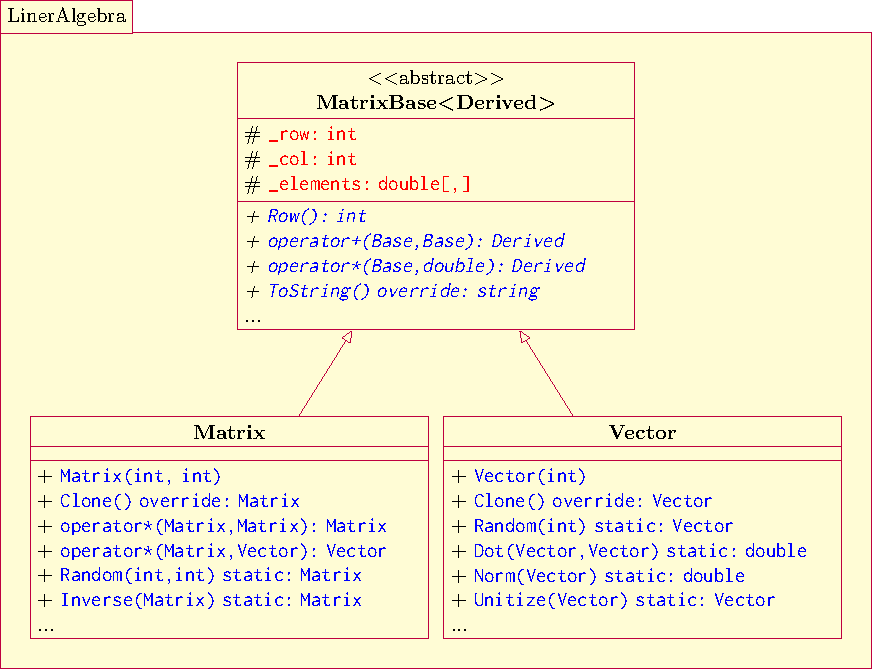
\includegraphics[scale=0.9]{Figures/MatrixClass.pdf}
\caption{矩阵向量类}
\label{fig:MatrixBaseClass}
\end{figure}
\noindent 由于图片限制,实际上\code{Matrix}类还继承于一个泛型接口\code{IMatrix<T>},接口的作用是利用泛型统一不同矩阵的同名函数,如\code{Transpose},\code{Inverse}函数等等,因为我特化了常用的三阶矩阵类\code{Matrix3d}.这样一来,就可以把\code{Matrix3d}类的\code{Transpose}函数和\code{Matrix}类的\code{Transpose}函数利用泛型封装在一个矩阵运算静态类中统一起来调用,例如:
\begin{lstlisting}[caption={\ttfamily MatrixOperate}\hspace{0pt}类]
internal static class MatrixOperate
{
    public static T Transpose<T>(T m) where T : IMatrix<T> => T.Transpose(m);
    public static double Trace<T>(T m) where T : IMatrix<T> => T.Trace(m);
    public static T Inverse<T>(T m) where T : IMatrix<T> => T.Inverse(m);
}
\end{lstlisting}
这样一来,不管矩阵\code{m}是\code{Matrix}类型的还是\code{Matrix3d}类型的都可以使用\code{MatrixOperate.Trace(m)}\\而不是分别使用\code{Matrix.Trace(m)}和\code{Matrix3d.Trace(m)}.对于向量类也有类似的接口\code{IVector<T>}.
\begin{figure}[H]
\centering
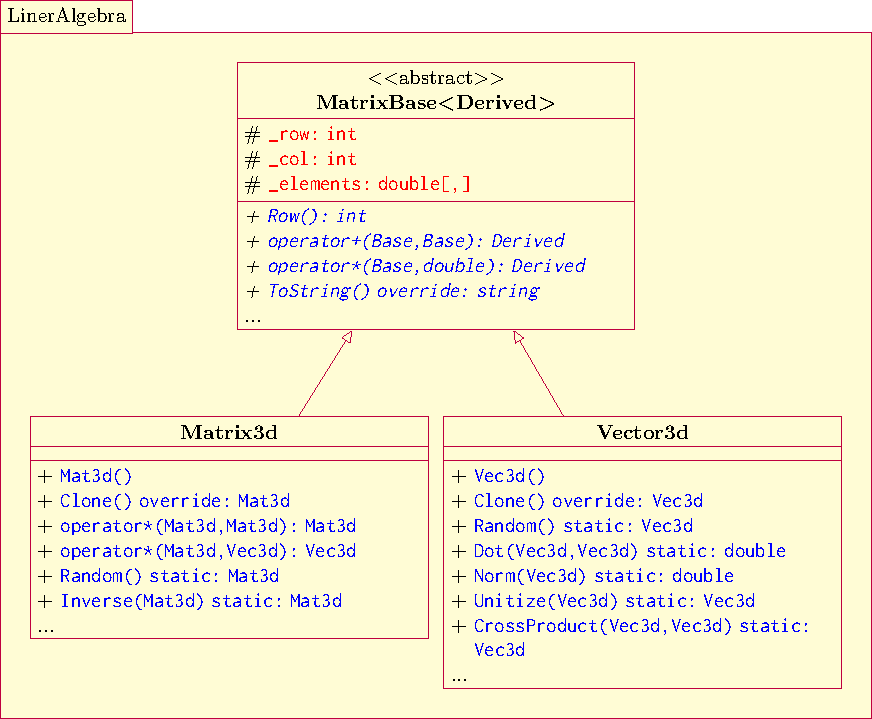
\includegraphics[scale=0.9]{Figures/Matrix3dClass.pdf}
\caption{三维矩阵/向量类}
\label{fig:Matrix3dClass}
\end{figure}
\noindent 当然,我也提供了从\code{Matrix3d}到\code{Matrix}的隐式转换与\code{Matrix}到\code{Matrix3d}的显示转换.

\subsection{姿态位置表示}
姿态更新使用四元数和等效旋转矢量法.所以我写了欧拉角类和四元数类,欧拉角类的字段除开三个欧拉角外,还有旋转矩阵,四元数类的字段即一个长度为$4$的数组,可以与四维向量\code{Vector4d}互相转换,与欧拉角互相转换,与等效旋转矢量(即一个\code{Vector3d})互相转换.如下图所示:
\begin{figure}[H]
\centering
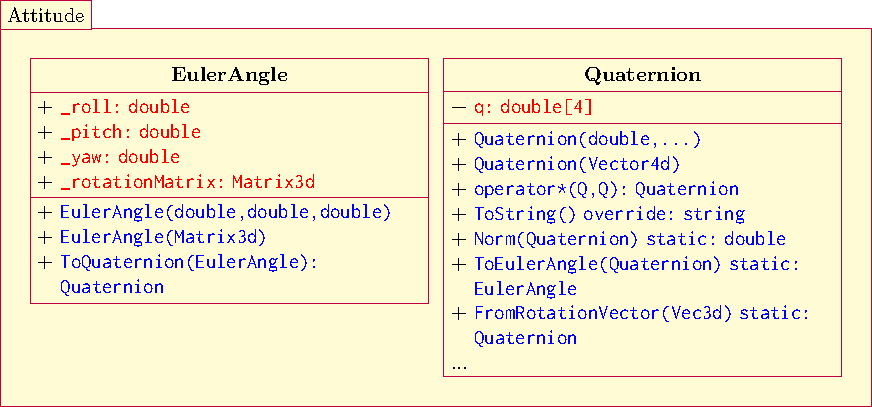
\includegraphics[scale=0.9]{Figures/EulerAngle.pdf}
\caption{姿态表示}
\label{fig:AttitudeClass}
\end{figure}
需要注意的是,在四元数转等效旋转矢量的时候,即使用公式\eqref{eq:rotationVecToQuaternion}的时候,如果$\phi=(0,0,0)$,那么程序会出现\code{NaN}的结果,实际上这是完全有可能的,因为IMU原始数据都是整型变量,若三轴陀螺输出均为$0$,那么从这个历元开始无法进行姿态更新.注意到
\[
    \lim_{\phi\to\boldsymbol{0}}q = 1 + \lim_{\phi\to\boldsymbol{0}}\frac{\sin \frac{|\phi|}{2}}{|\phi|}\phi
    = 1 + 0i + 0j + 0k = 1,
\]
所以在$\phi=\boldsymbol{0}$的时候应该把对应的四元数设置为$1$.代码如下:
\begin{lstlisting}[caption=等效旋转矢量转四元数]
public static Quaternion FromRotationVector(Vector3d vector)
{
    double norm = VectorOperate.Norm(vector);
    if (norm < 1e-14)
    {
        return new(1, 0, 0, 0);
    }
    double halfAngle = norm * 0.5;
    double s = Math.Sin(halfAngle);
    double c = Math.Cos(halfAngle);
    Vector3d unitVector = VectorOperate.Unitize(vector);
    return new(c, unitVector[0] * s, unitVector[1] * s, unitVector[2] * s);
}
\end{lstlisting}

对于位置,采用BLH坐标系,类的设计也很简单,\code{BLHCoordinate}类的成员就是三个\code{double}类型的自动属性.然后重写了\code{ToString()}方法.

对于参考椭球,设计了一个名为\code{CoordinateSystem}的枚举类型以及一个名为\code{Elliposid}的类,里面包含了表\ref{tab:GRS80}中的六个椭球参数,使用\code{CoordinateSystem}作为构造函数的参数.

\subsection{更新算法}\label{sec:4.3}

首先我们需要对\textsf{IMU}输出的数据进行存储,故设计一个\code{IMUData}类,其中有一个\code{const}成员为\textsf{IMU}的采样率,还有两个只读的静态成员\code{acc_scale}和\code{gyro_scale}.剩下的有一个\code{double}类型的属性表示当前历元的周内秒,还有两个类型为\code{Vector3d}的成员分别为角度增量和速度增量.

对于更新算法,我们还需要设计一个类描述和记录当前历元的结算结果,即速度位置和姿态.所以定义类\code{MotionState}.其中还包含一些计算用到的辅助量,例如$R_M$和$\omega_{ie}^n$等.
\begin{figure}[H]
\centering
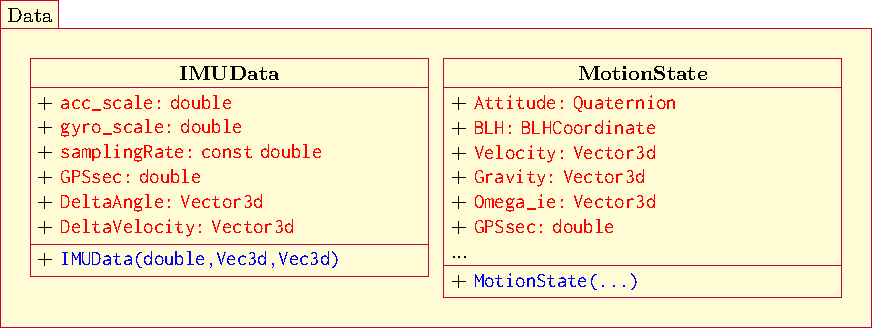
\includegraphics[scale=0.9]{Figures/DataClass.pdf}
\caption{一些数据类}
\label{fig:DataClass}
\end{figure}

对于更新算法,按照\ref{sec:INS}节的公式进行编写即可:
\begin{lstlisting}
public static MotionState Update(MotionState mBack, MotionState mBBack, IMUData dataNow, IMUData dataBack)
{
    deltaT = IMUData.SamplingRate;
    Quaternion attitude = AttitudeUpdate(mBack, dataBack, dataNow);
    Vector3d velocity = VelocityUpdate(mBBack, mBack, dataBack, dataNow);
    BLHCoordinate position = PositionUpdate(mBack, mBBack, velocity);
    return new MotionState(attitude, position, velocity, dataNow.GPSsec);
}
\end{lstlisting}
其中\code{AttitudeUpdate},\code{VelocityUpdate},\code{PositionUpdate}函数分别对应三个更新公式.\code{Update}函数\\包含在一个静态类\code{INSAlgorithm}中:
\begin{lstlisting}
internal static class INSAlgorithm
{
    private static double deltaT;
    public static MotionState Update(MotionState, MotionState, IMUData, IMUData);
    private static Quaternion AttitudeUpdate(MotionState, IMUData, IMUData);
    private static Vector3d VelocityUpdate(MotionState, MotionState, IMUData, IMUData);
    private static BLHCoordinate PositionUpdate(MotionState, MotionState, Vector3d);
}
\end{lstlisting}

\subsection{数据处理}
本次实验需要处理两组数据,一组是参考数据和参考数据的结果用于验证程序的正确性,另一组是实验数据和实验数据的结果用于分析.由于涉及到大量数据的处理,所以我选择在程序中直接打开\textsf{Excel}导出计算结果和参考结果到一张工作表上,便于后续绘图.

如果计算机已安装\textsf{Excel},在\code{C\#}项目中,可以添加名为\textsf{Microsoft Excel 16.0 Object Library}的\textsf{COM}组件引用.
然后就可以在项目里面使用命名空间\code{Microsoft.Office.Interop.Excel}.创建一个工作簿的代码如下:
\begin{lstlisting}
//using Excel = Microsoft.Office.Interop.Excel;
Excel.Application excel = new()
{
    Visible = true,
};
Excel.Workbooks workbooks = excel.Workbooks;
Excel.Workbook workbook = workbooks.Add(Excel.XlWBATemplate.xlWBATWorksheet);
\end{lstlisting}
为了提高代码的复用性,将创建表单和向表单中添加数据的操作封装为一个静态类\code{ExportExcel}:
\begin{lstlisting}
internal static class ExportExcel
{
    public static Excel.Worksheet GetExcel(Excel.Workbook workbook, string workSheetName, string[] sheetHeader, double[,] data, int row, int col);
    public static void AddExcel(Excel.Worksheet worksheet, Excel.Range startCell, string[] sheetHeader, double[,] data, int row, int col);
}
\end{lstlisting}
\code{GetExcel}函数的作用是根据\textsf{IMU}数据进行更新算法后得出的二维数组创建一个属于上面工作簿的新表单.\code{AddExcel}函数的作用是将二维数组中的数据添加到已有表单的某个位置,用于把参考结果放到与解算结果相同的表单中.

对于实验数据和示例数据,它们的计算过程完全一致,但是实际编写程序的时候又有区别.例如示例数据是二进制文件读取,不需要零速修正,但是它们更新算法相同,导出\textsf{Excel}的格式相同.所以使用多态来设计数据的处理部分.使用一个抽象类\code{DataBase}来作为二进制数据类和\textsf{ASC}数据类的父类.存放一个二位数组作为计算结果或者参考结果的载体,以及计算所需的必要数据,如当前时刻,上一时刻和上两个时刻的运动状态,当前时刻和上一时刻的\textsf{IMU}数据,即\ref{sec:4.3}节中提到的\code{MotionState}和\code{IMUData}类.然后是一些方法,如\code{Update}方法,用于更新算法调用\ref{sec:4.3}节的\code{INSAlgorithm.Update}方法;\code{IMUDataCal}方法,用于计算\textsf{IMU}更新结果并赋值给二维数组;\code{ReferenceRead}方法,用于读取参考数据;\code{CalAndExportExcel}方法,用于一次性完成计算\textsf{IMU}数据,读取参考结果与导出\textsf{Excel}表格三件事.此外,\code{DataBase}类还含有一个\code{Func<double, bool>?}类型的委托(类似于\code{C++}的函数指针),如果它为\code{null},表明不进行零速修正,否则根据自定义零速修正的区间进行零速修正.

这样设计的好处在于,在保证实现基本功能的情况下,减少了代码量并大大提高了可读性,使实验数据和示例数据在互相分离的同时又可以通过多态提供的统一接口去调用,并且提供了丰富的选项去设置:主函数设置初始状态,\textsf{IMU}采样率,是否计算站心坐标,定义零速修正规则(传给上述委托).再通过\code{DataBase}父类创建对应的子类对象,再调用\code{CalAndExportExcel}方法即可生成最后的结果:
\newpage
\begin{lstlisting}[caption=主函数代码]
//获取示例数据的计算结果与参考结果
{
    DataBase data = new BinaryData(/*初始状态*/, /*采样率*/, /*数组最大行数*/, /*是否计算站心坐标*/);
    data.CalAndExportExcel("IMUPath", "ReferencePath");
}
//获取实验数据的计算结果与参考结果
{
    Func<double, bool> zeroVelCorrect = /*零速修正*/;
    DataBase data = new ASCData(/*初始状态*/, /*采样率*/, /*数组最大行数*/, /*是否计算站心坐标*/, /*是否零速修正*/);
    data.CalAndExportExcel("IMUPath", "ReferencePath");
}
\end{lstlisting}
可以发现二者的结构完全一致.其中\code{ASCData}和\code{BinaryData}的构造函数均有默认参数:默认计算站心坐标,不进行零速修正.基于上述的思路给出的类图如下:
\begin{figure}[H]
\centering
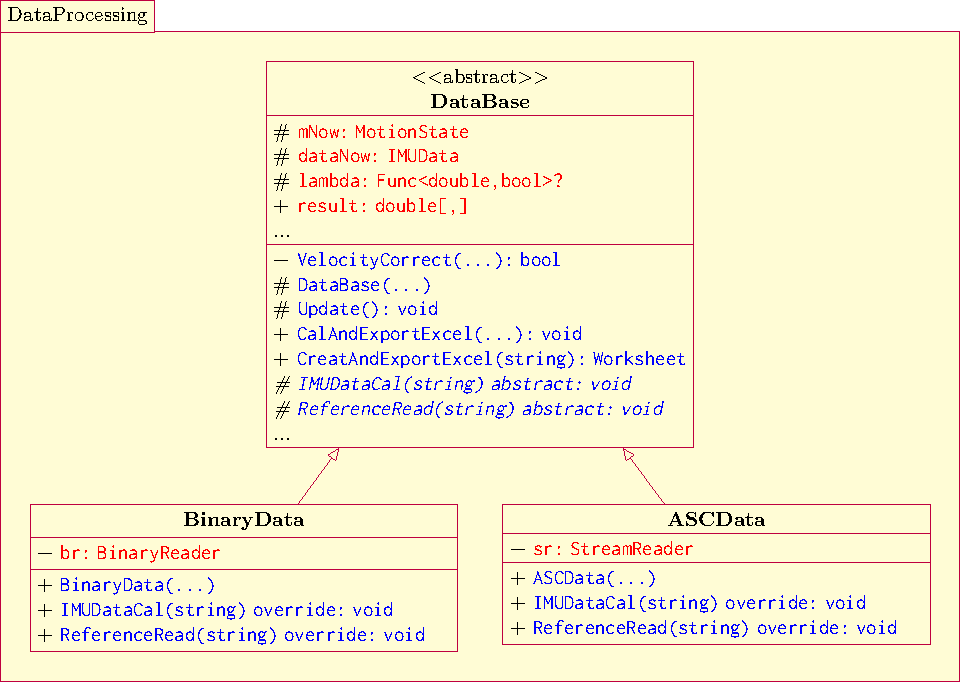
\includegraphics[scale=0.9]{Figures/DataBaseClass.pdf}
\caption{数据处理}
\label{fig:DataProcessing}
\end{figure}
在导出\textsf{Excel}的时候需要注意避免使用\code{for}循环填充单个单元格,应该直接把二维数组的所有数据内存转移给一个\code{Excel.Range},实际测试中只需要20余秒便能完成示例数据七十多万个历元的计算,参考数据的读取并全部导出为\textsf{Excel}.

\section{示例数据运行结果}

生成示例数据的解算结果与参考结果表格用时23s.将示例数据的经纬度,椭球高,速度,姿态角分别与参考结果的对应项做差,得出图\ref{fig:5.1}(由于\textsf{IMU}的采样率是固定的,所以图片的横坐标统一表示当前历元的序号).
\begin{figure}[H]
    \centering
    {
        \captionsetup{textfont={footnotesize,tt}}
        \begin{subfigure}{0.49\textwidth}
            \centering
            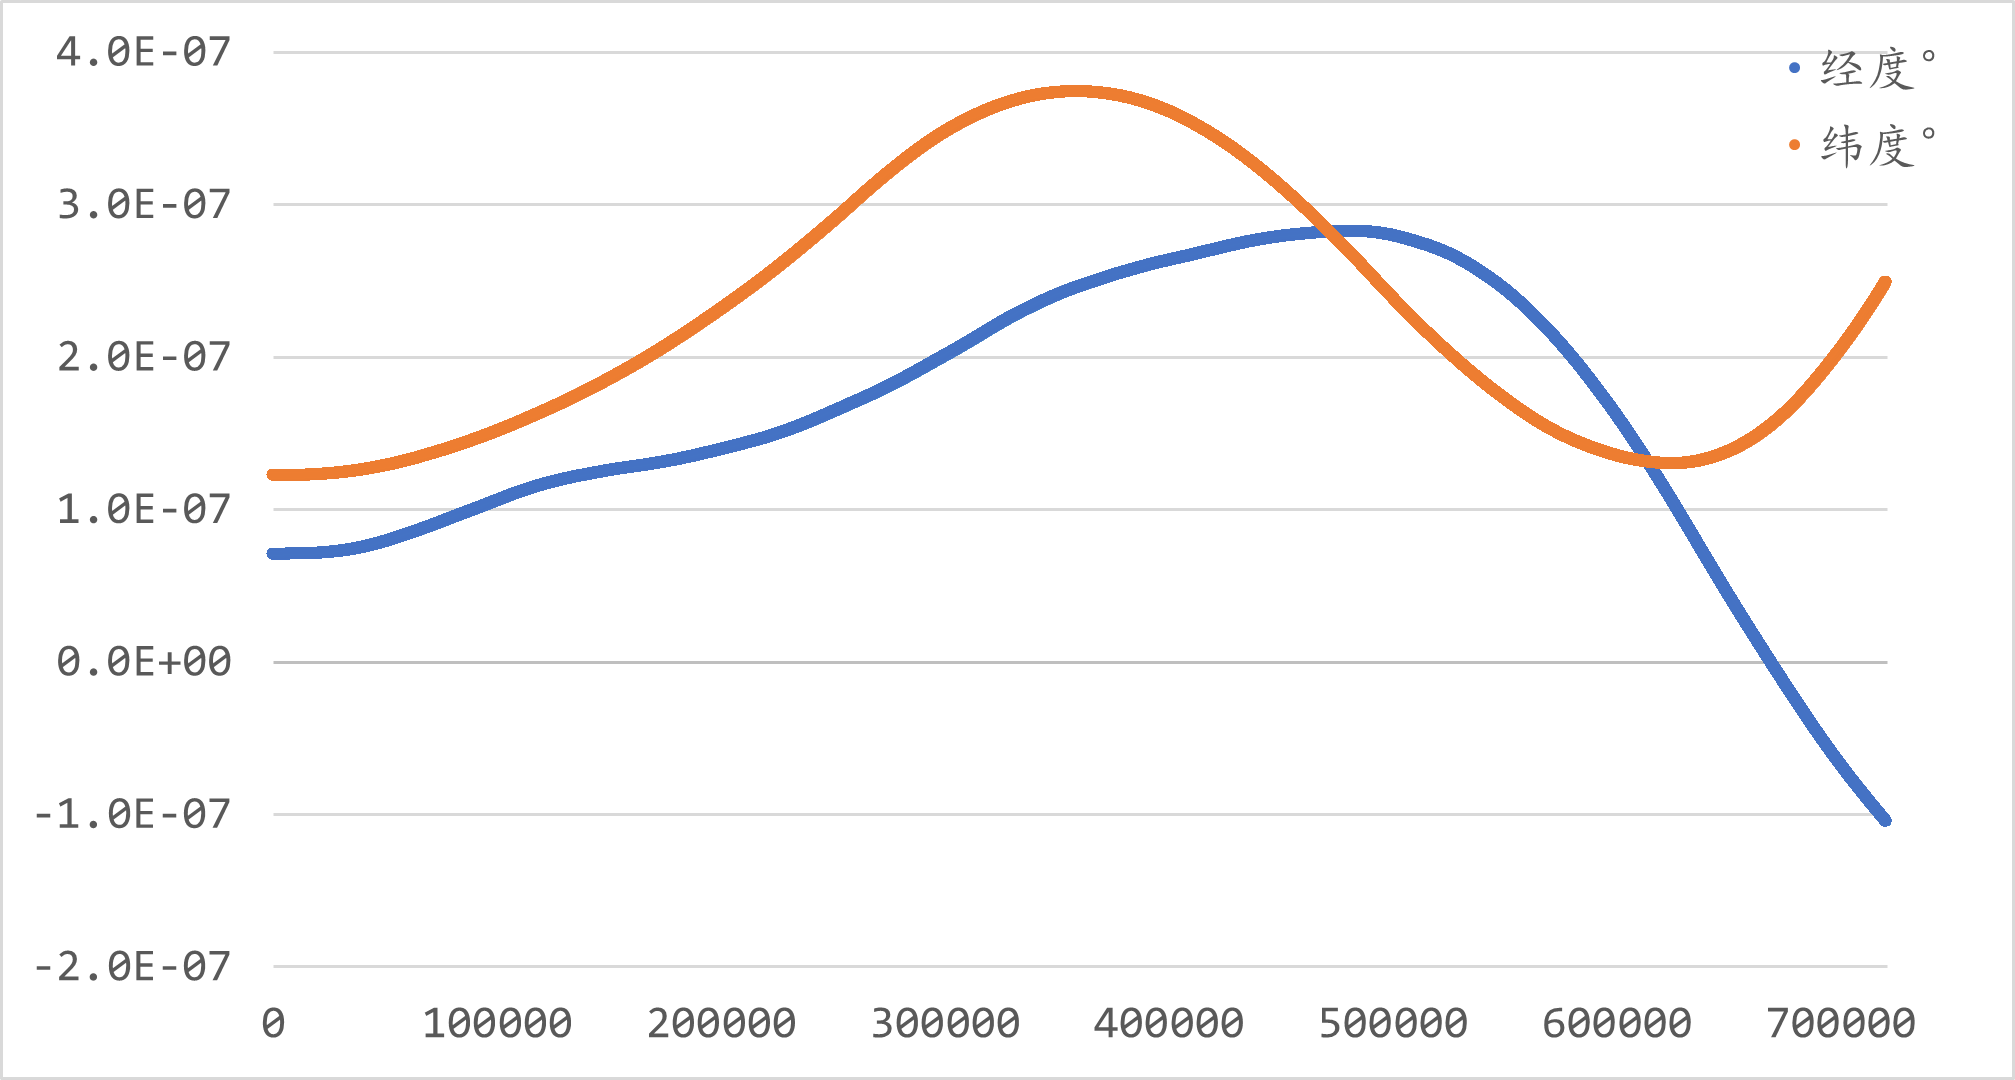
\includegraphics[width=\linewidth]{Figures/DataFigure/示例数据经纬度差异.png}
            \caption*{经纬度差异}
        \end{subfigure}\hfill
        \begin{subfigure}{0.49\textwidth}
            \centering
            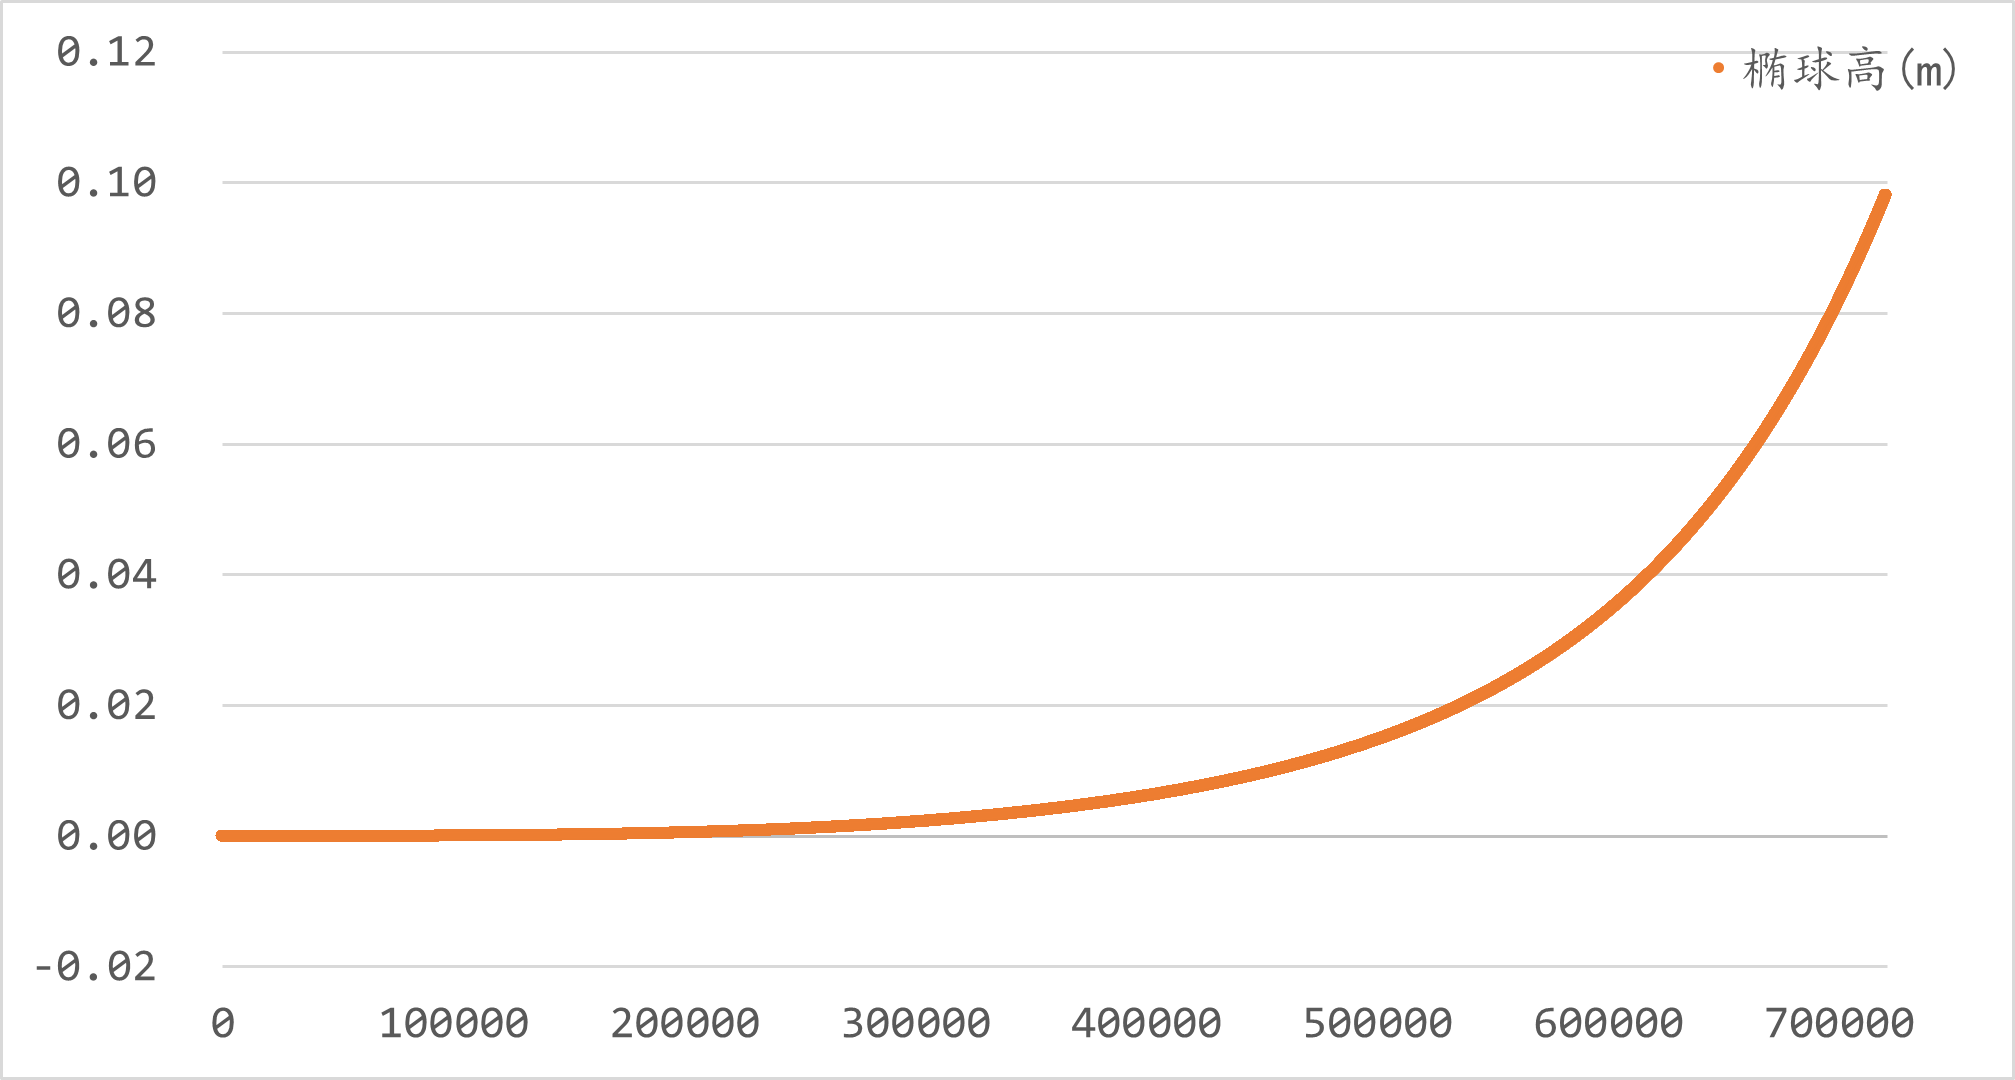
\includegraphics[width=\linewidth]{Figures/DataFigure/示例数据椭球高差异.png}
            \caption*{椭球高差异}
        \end{subfigure}
        
        \begin{subfigure}{0.49\textwidth}
            \centering
            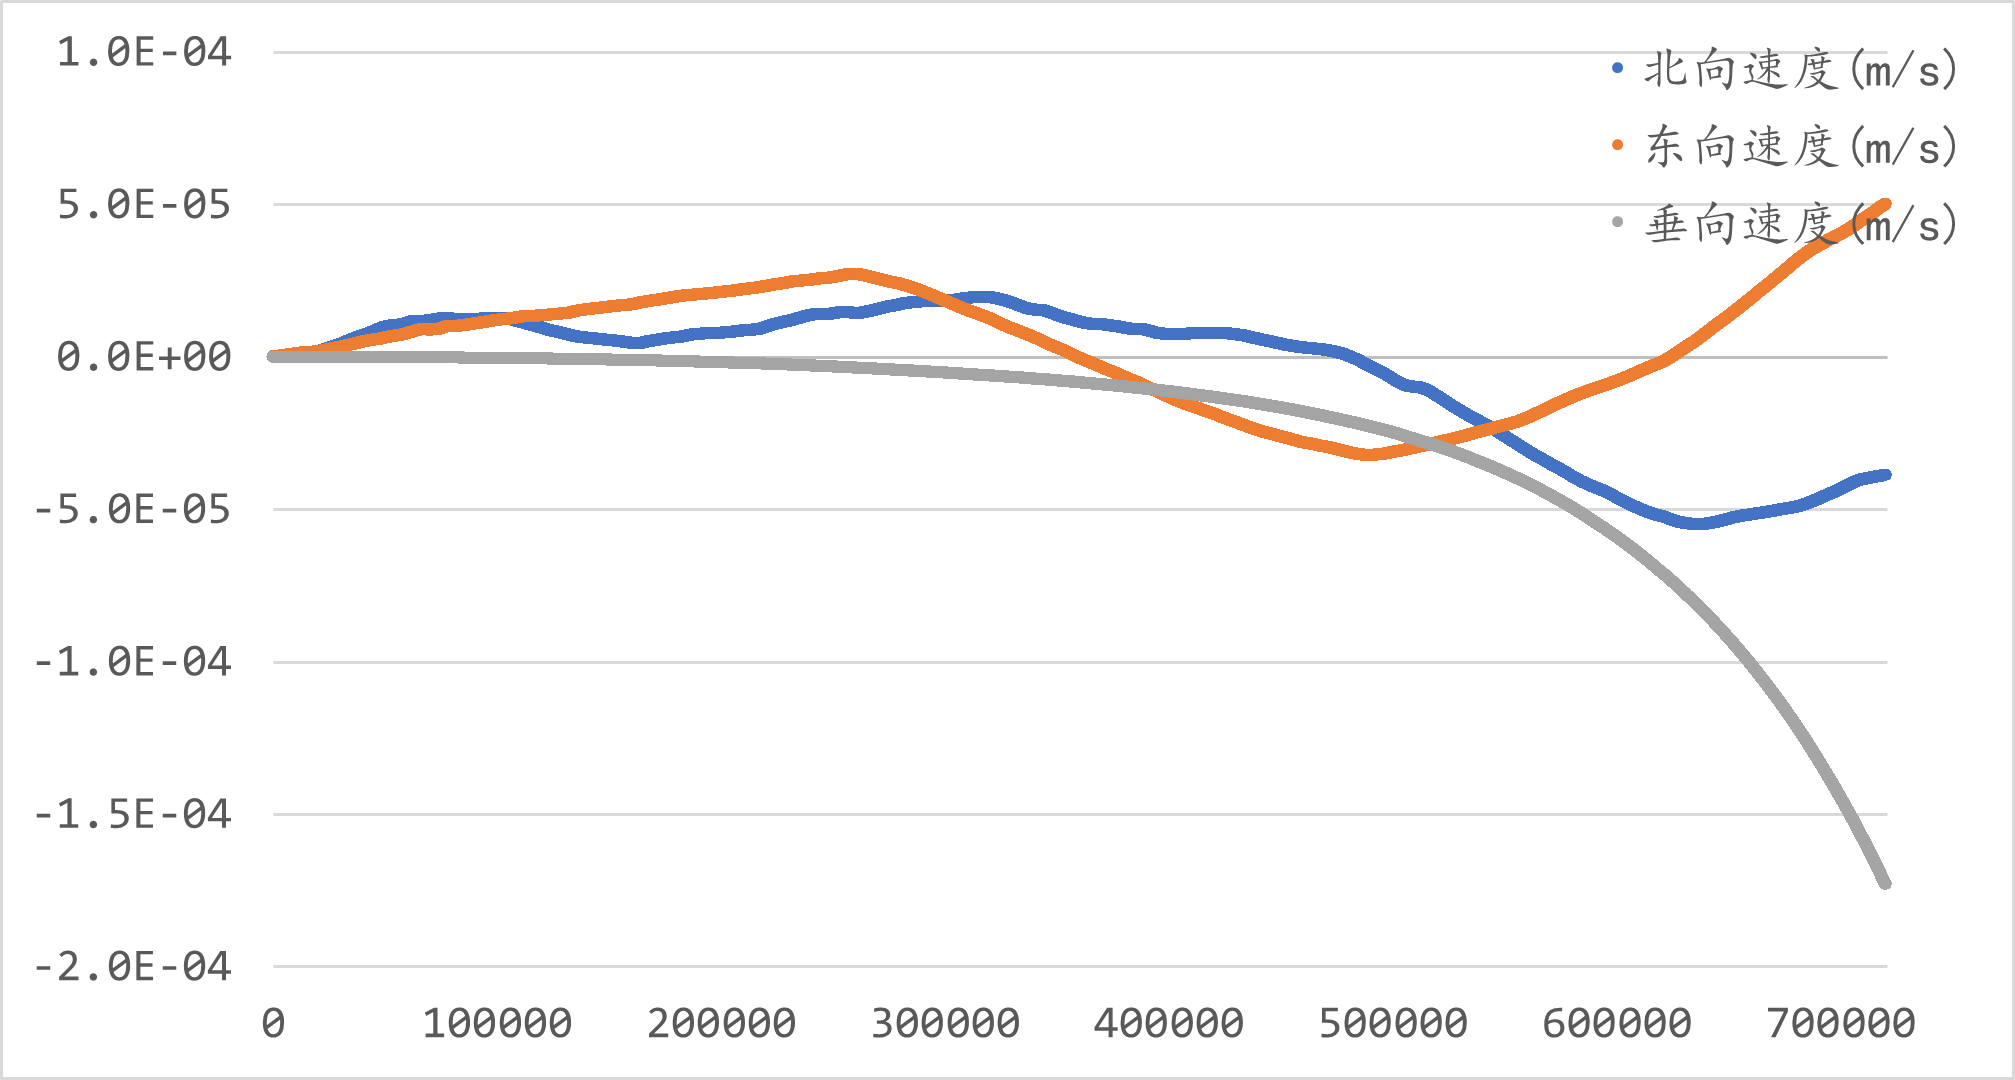
\includegraphics[width=\linewidth]{Figures/DataFigure/示例数据速度差异.png}
            \caption*{速度差异}
        \end{subfigure}\hfill
        \begin{subfigure}{0.49\textwidth}
            \centering
            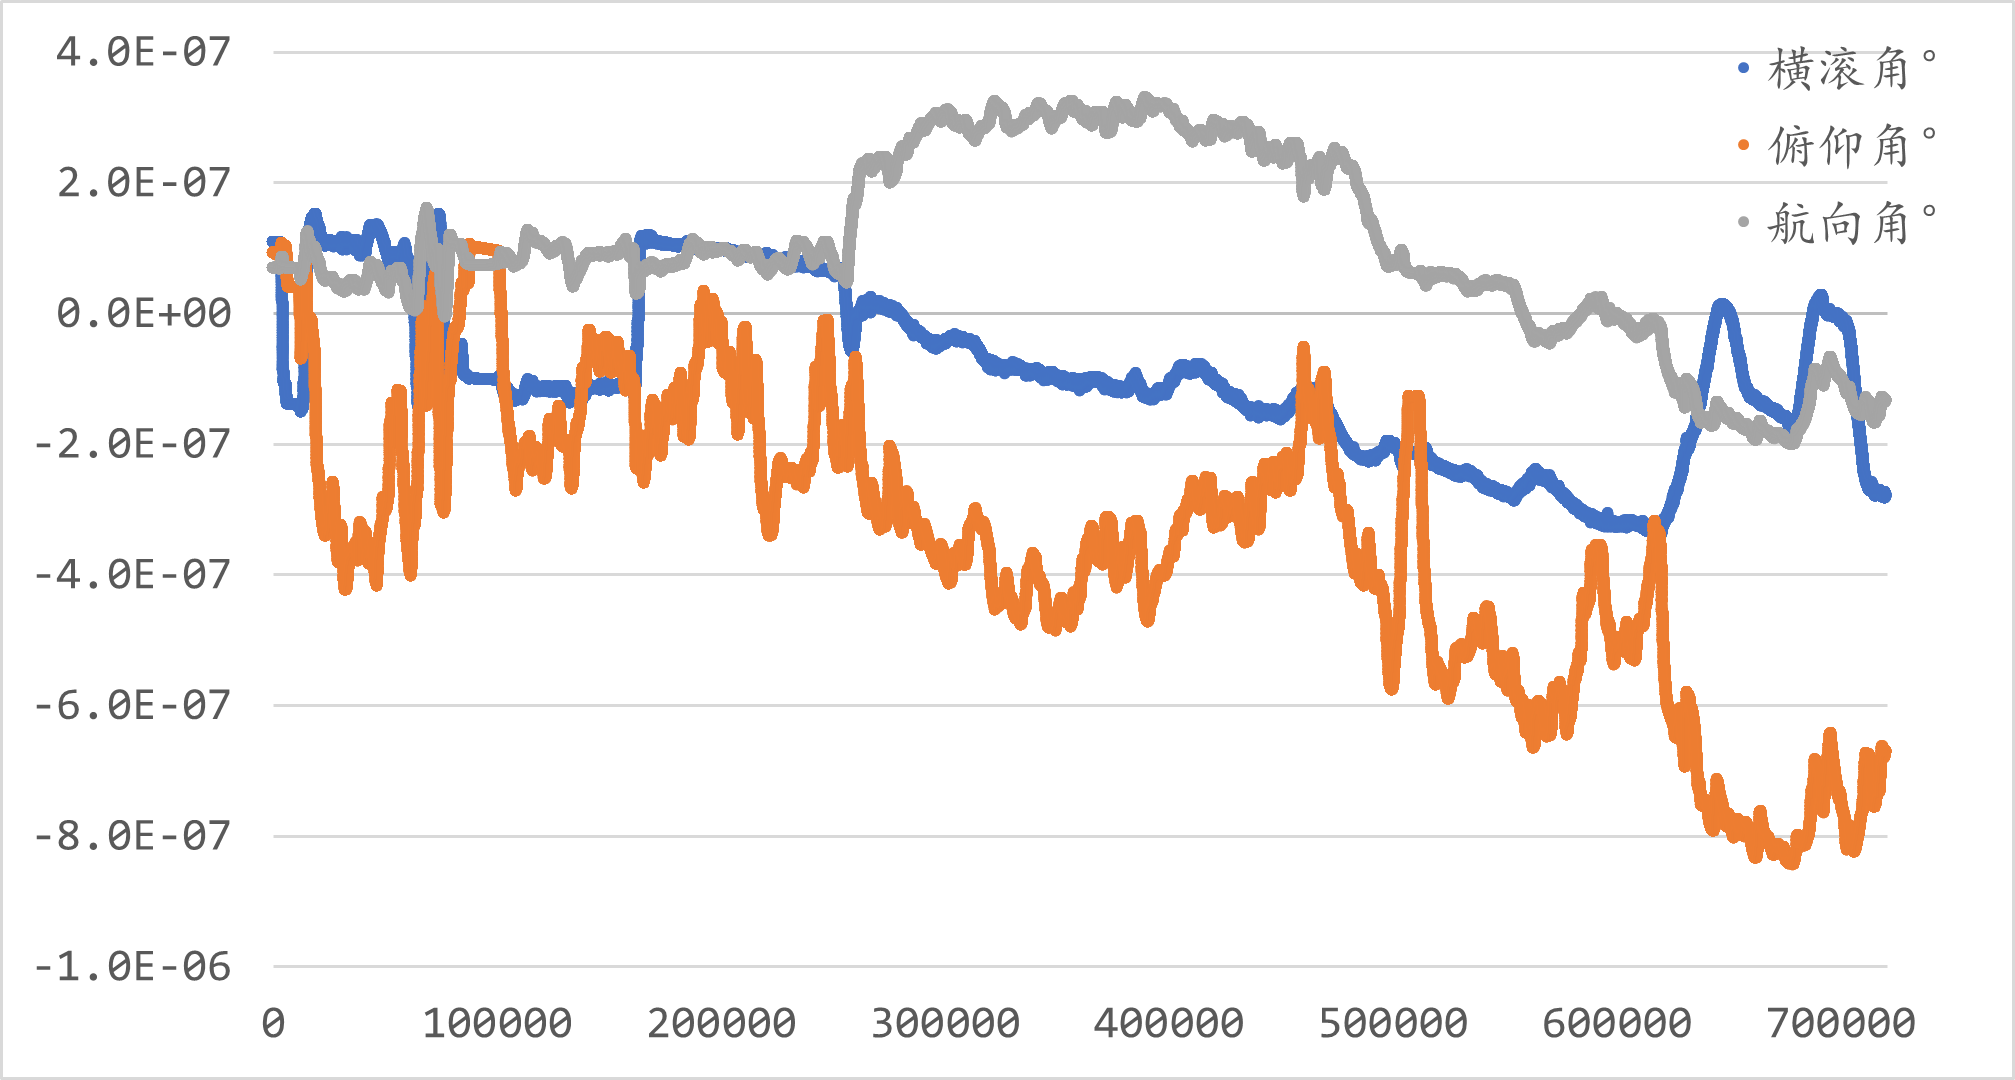
\includegraphics[width=\linewidth]{Figures/DataFigure/示例数据姿态角差异.png}
            \caption*{姿态角差异}
        \end{subfigure}
    }
    \caption{示例数据与参考结果差异}
    \label{fig:5.1}
\end{figure}
\noindent 经纬度的差异处于$10^{-7}$数量级,高程差异小于$0.1$m,速度差异处于$10^{-4}$数量级,姿态角处于$10^{-7}$数量级,均满足\ref{subsec:3.1}节的要求.对于示例数据,我也计算了它们的轨迹,如图\ref{fig:5.3}所示,可以发现它们基本一致,所以可以认为程序的算法无误.示例数据的垂向速度和椭球高变化如图\ref{fig:5.2}所示,在没有零速修正的情况下,经过约一个小时的纯惯导解算,垂向速度依然没有发散,可见示例数据采用的\textsf{IMU}精度是比较高的.
\begin{figure}[H]
    \centering
    {
        \captionsetup{textfont={footnotesize,tt}}
        \begin{subfigure}{0.49\textwidth}
            \centering
            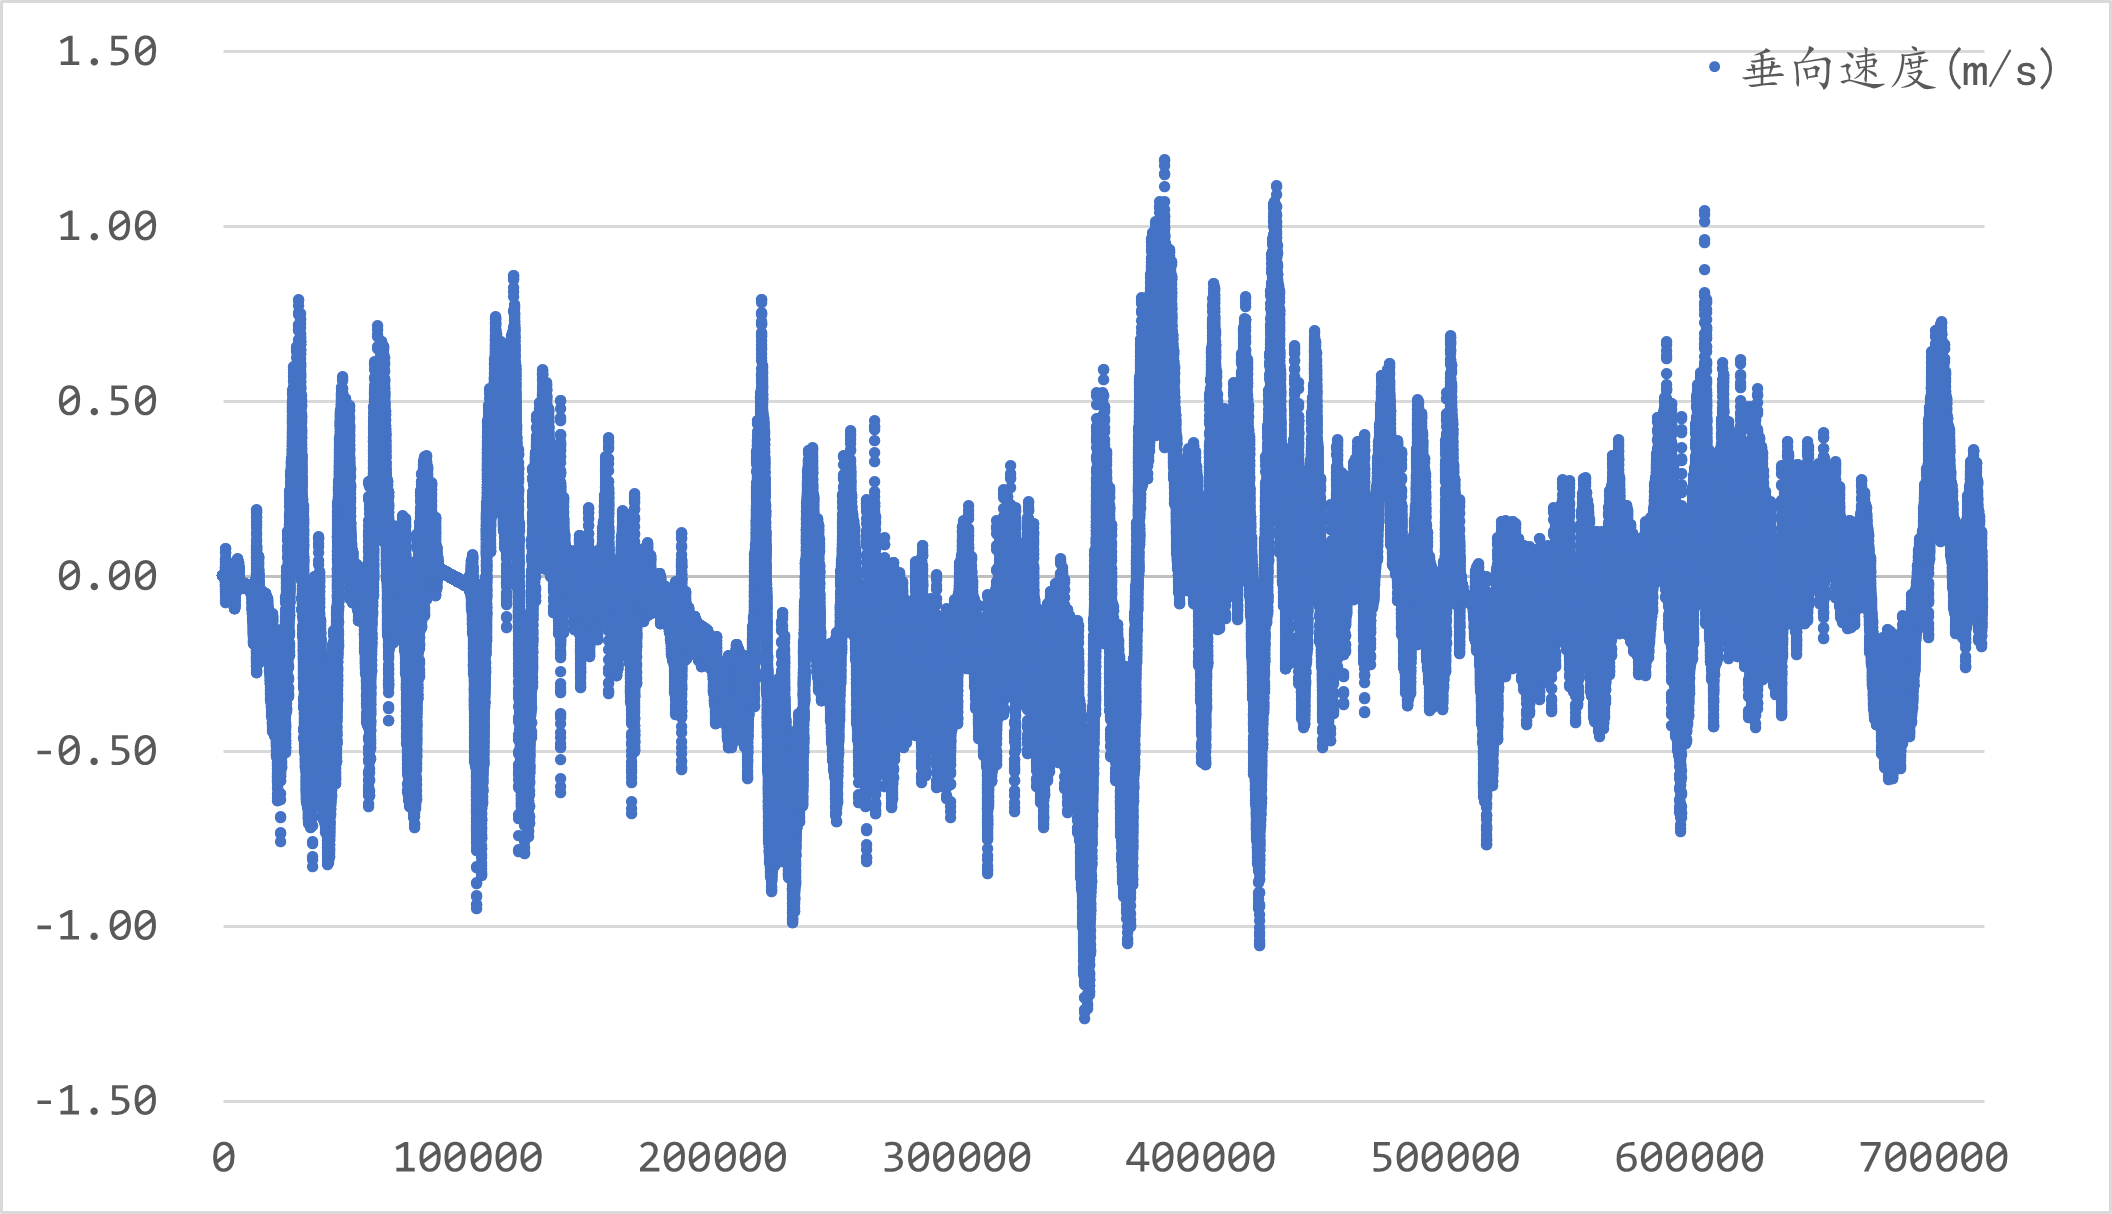
\includegraphics[width=\linewidth]{Figures/DataFigure/示例数据垂向速度.png}
        \end{subfigure}\hfill
        \begin{subfigure}{0.49\textwidth}
            \centering
            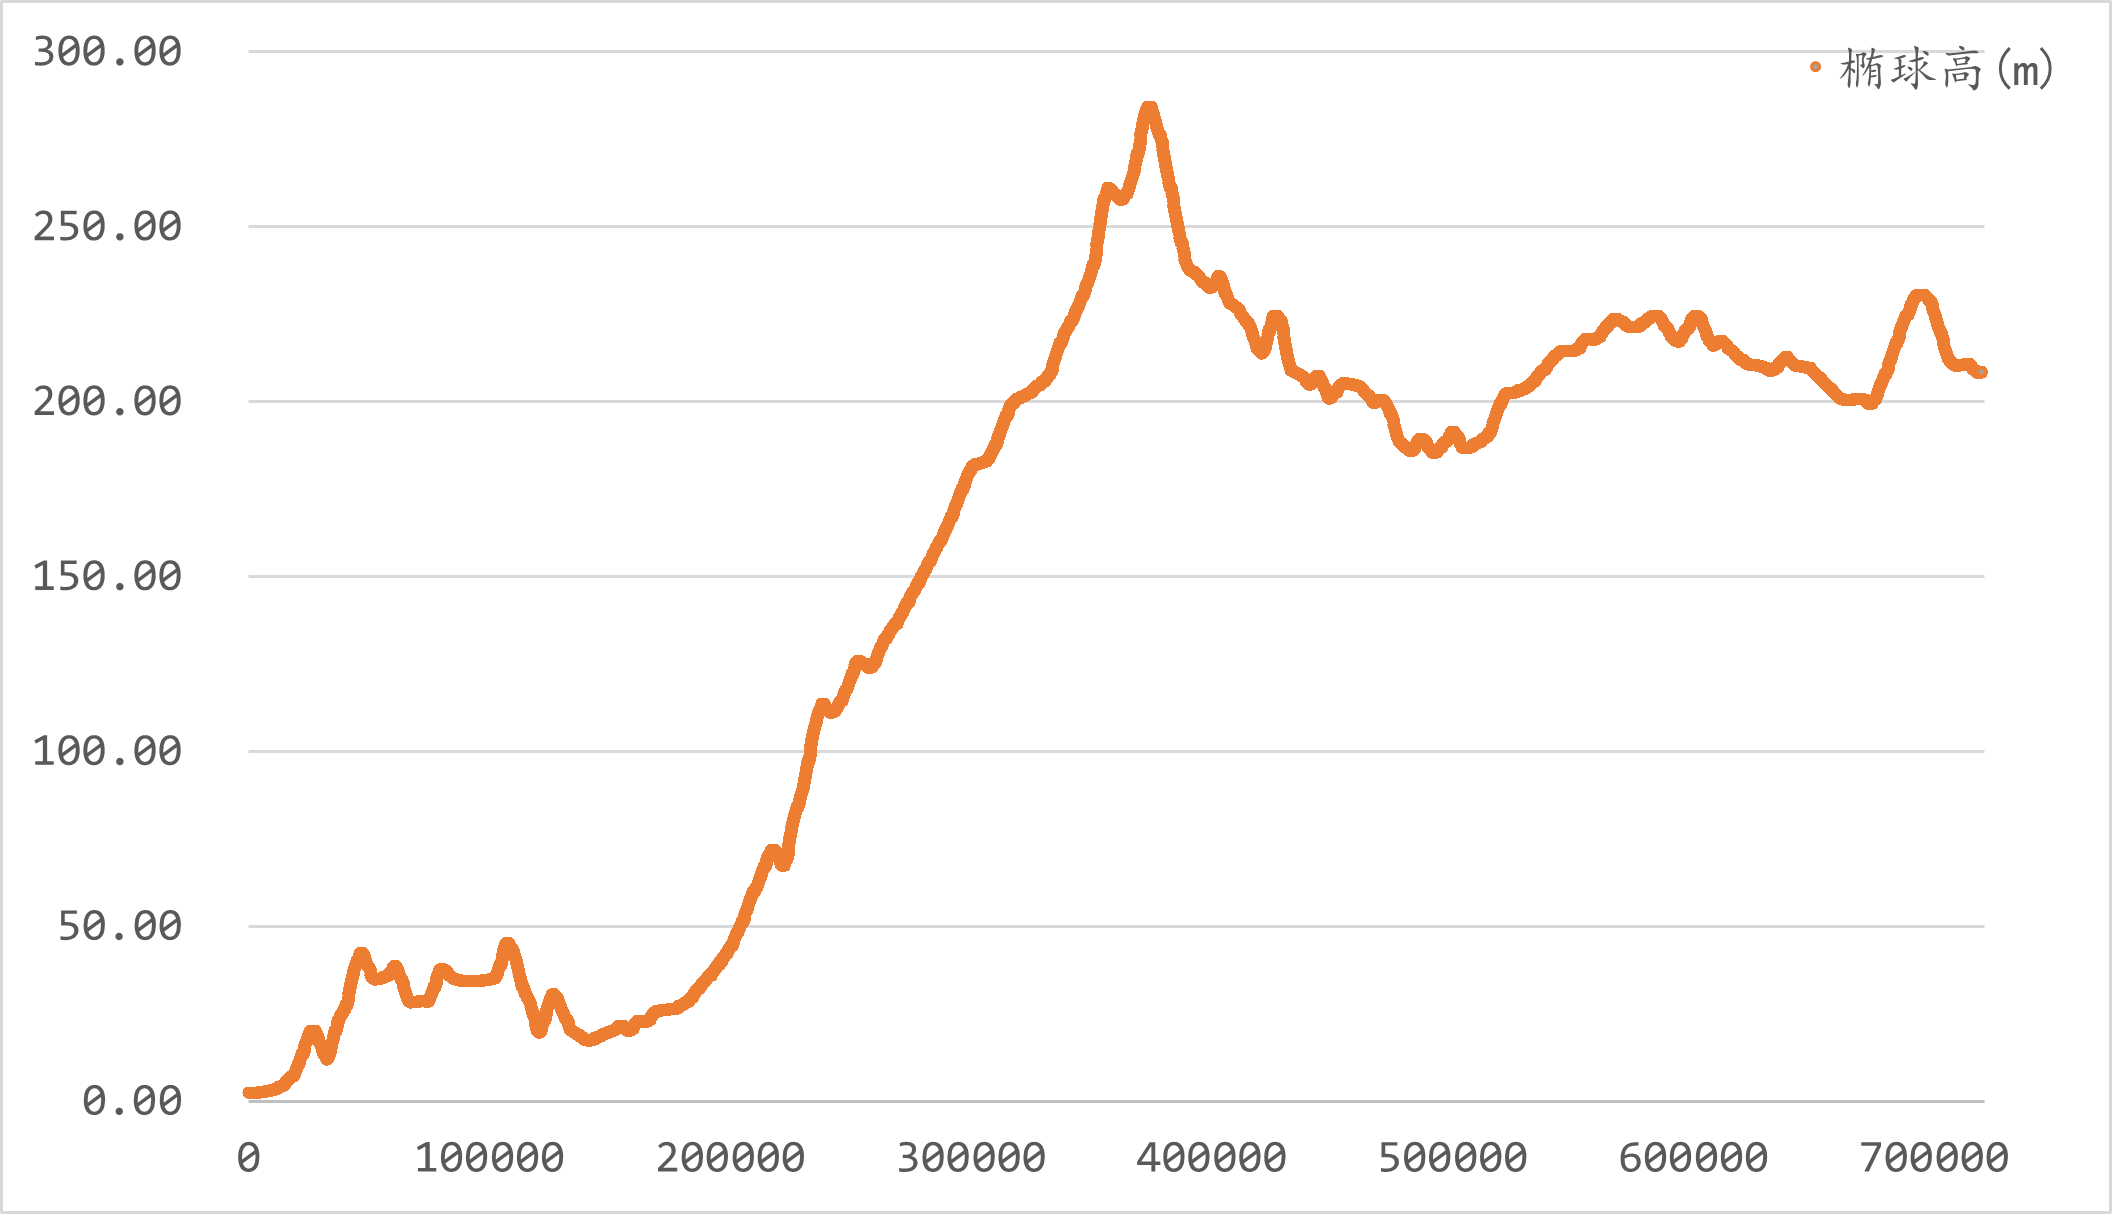
\includegraphics[width=\linewidth]{Figures/DataFigure/示例数据椭球高.png}
        \end{subfigure}
    }
    \caption{示例数据垂向数据}
    \label{fig:5.2}
\end{figure}
\begin{figure}[H]
    \centering
    {
        \captionsetup{textfont={footnotesize,tt}}
        \begin{subfigure}{0.49\textwidth}
            \centering
            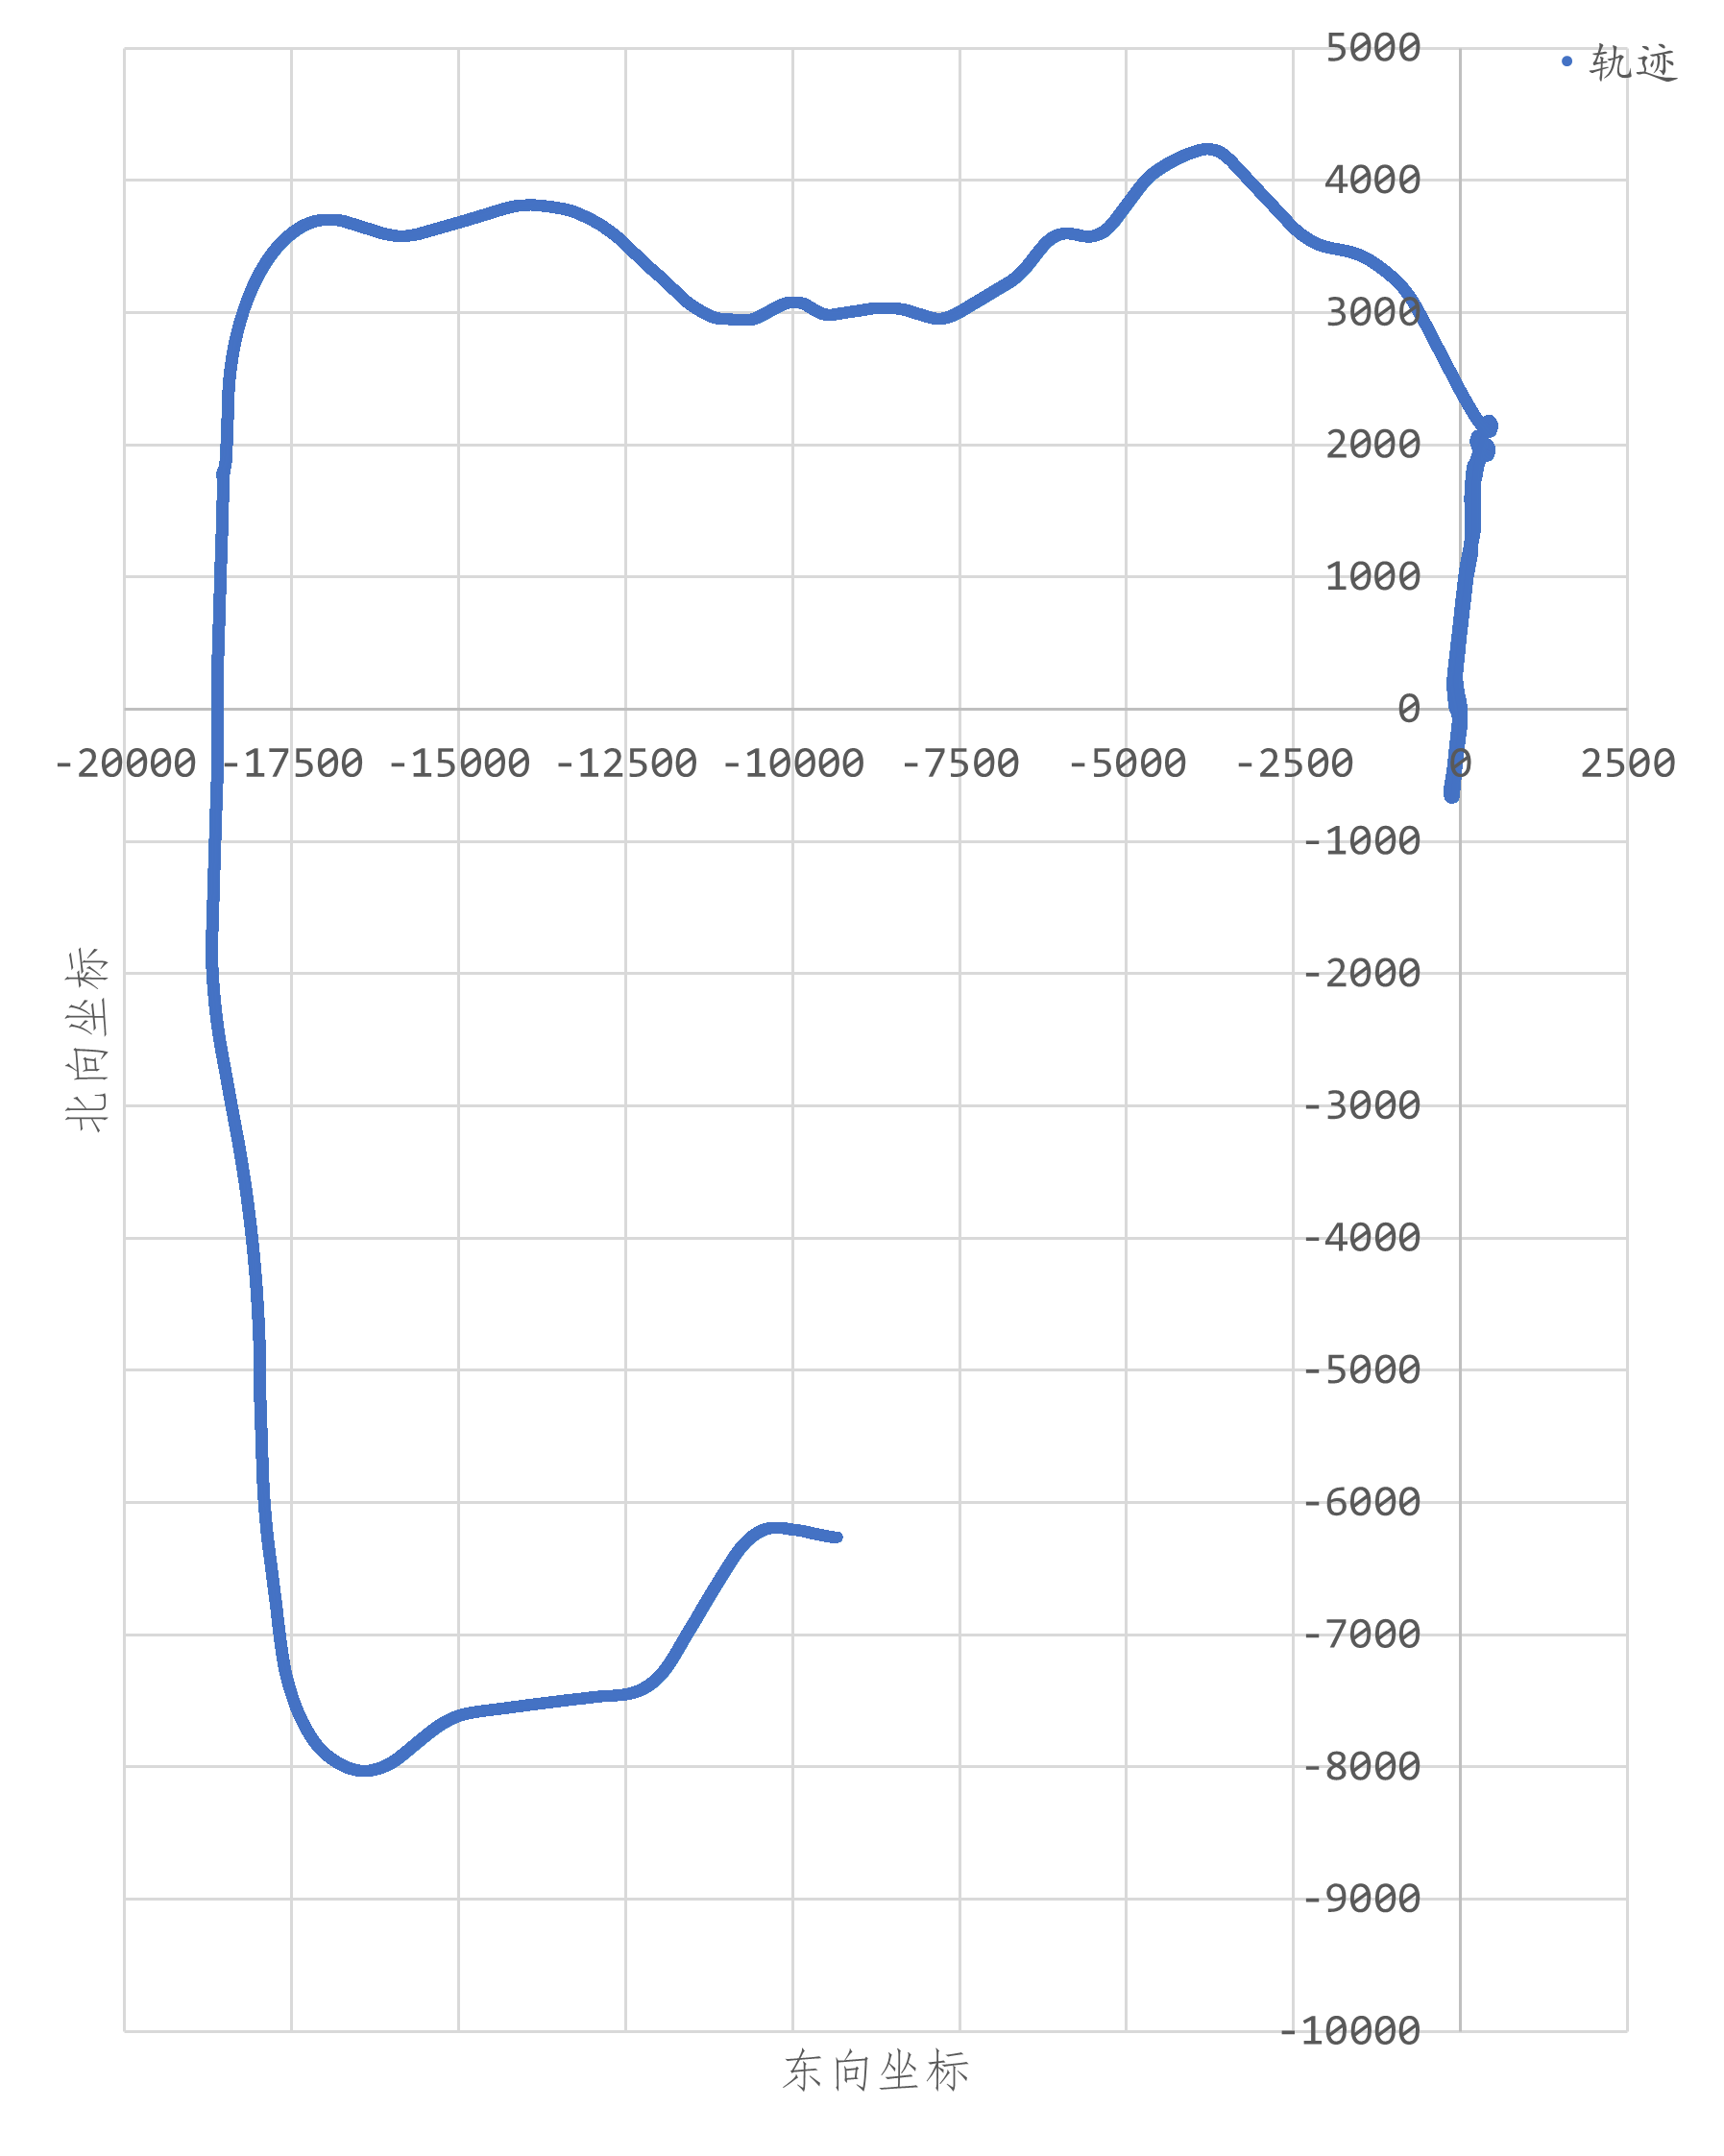
\includegraphics[width=\linewidth]{Figures/DataFigure/示例数据解算轨迹.png}
            \caption*{程序计算轨迹}
        \end{subfigure}\hfill
        \begin{subfigure}{0.49\textwidth}
            \centering
            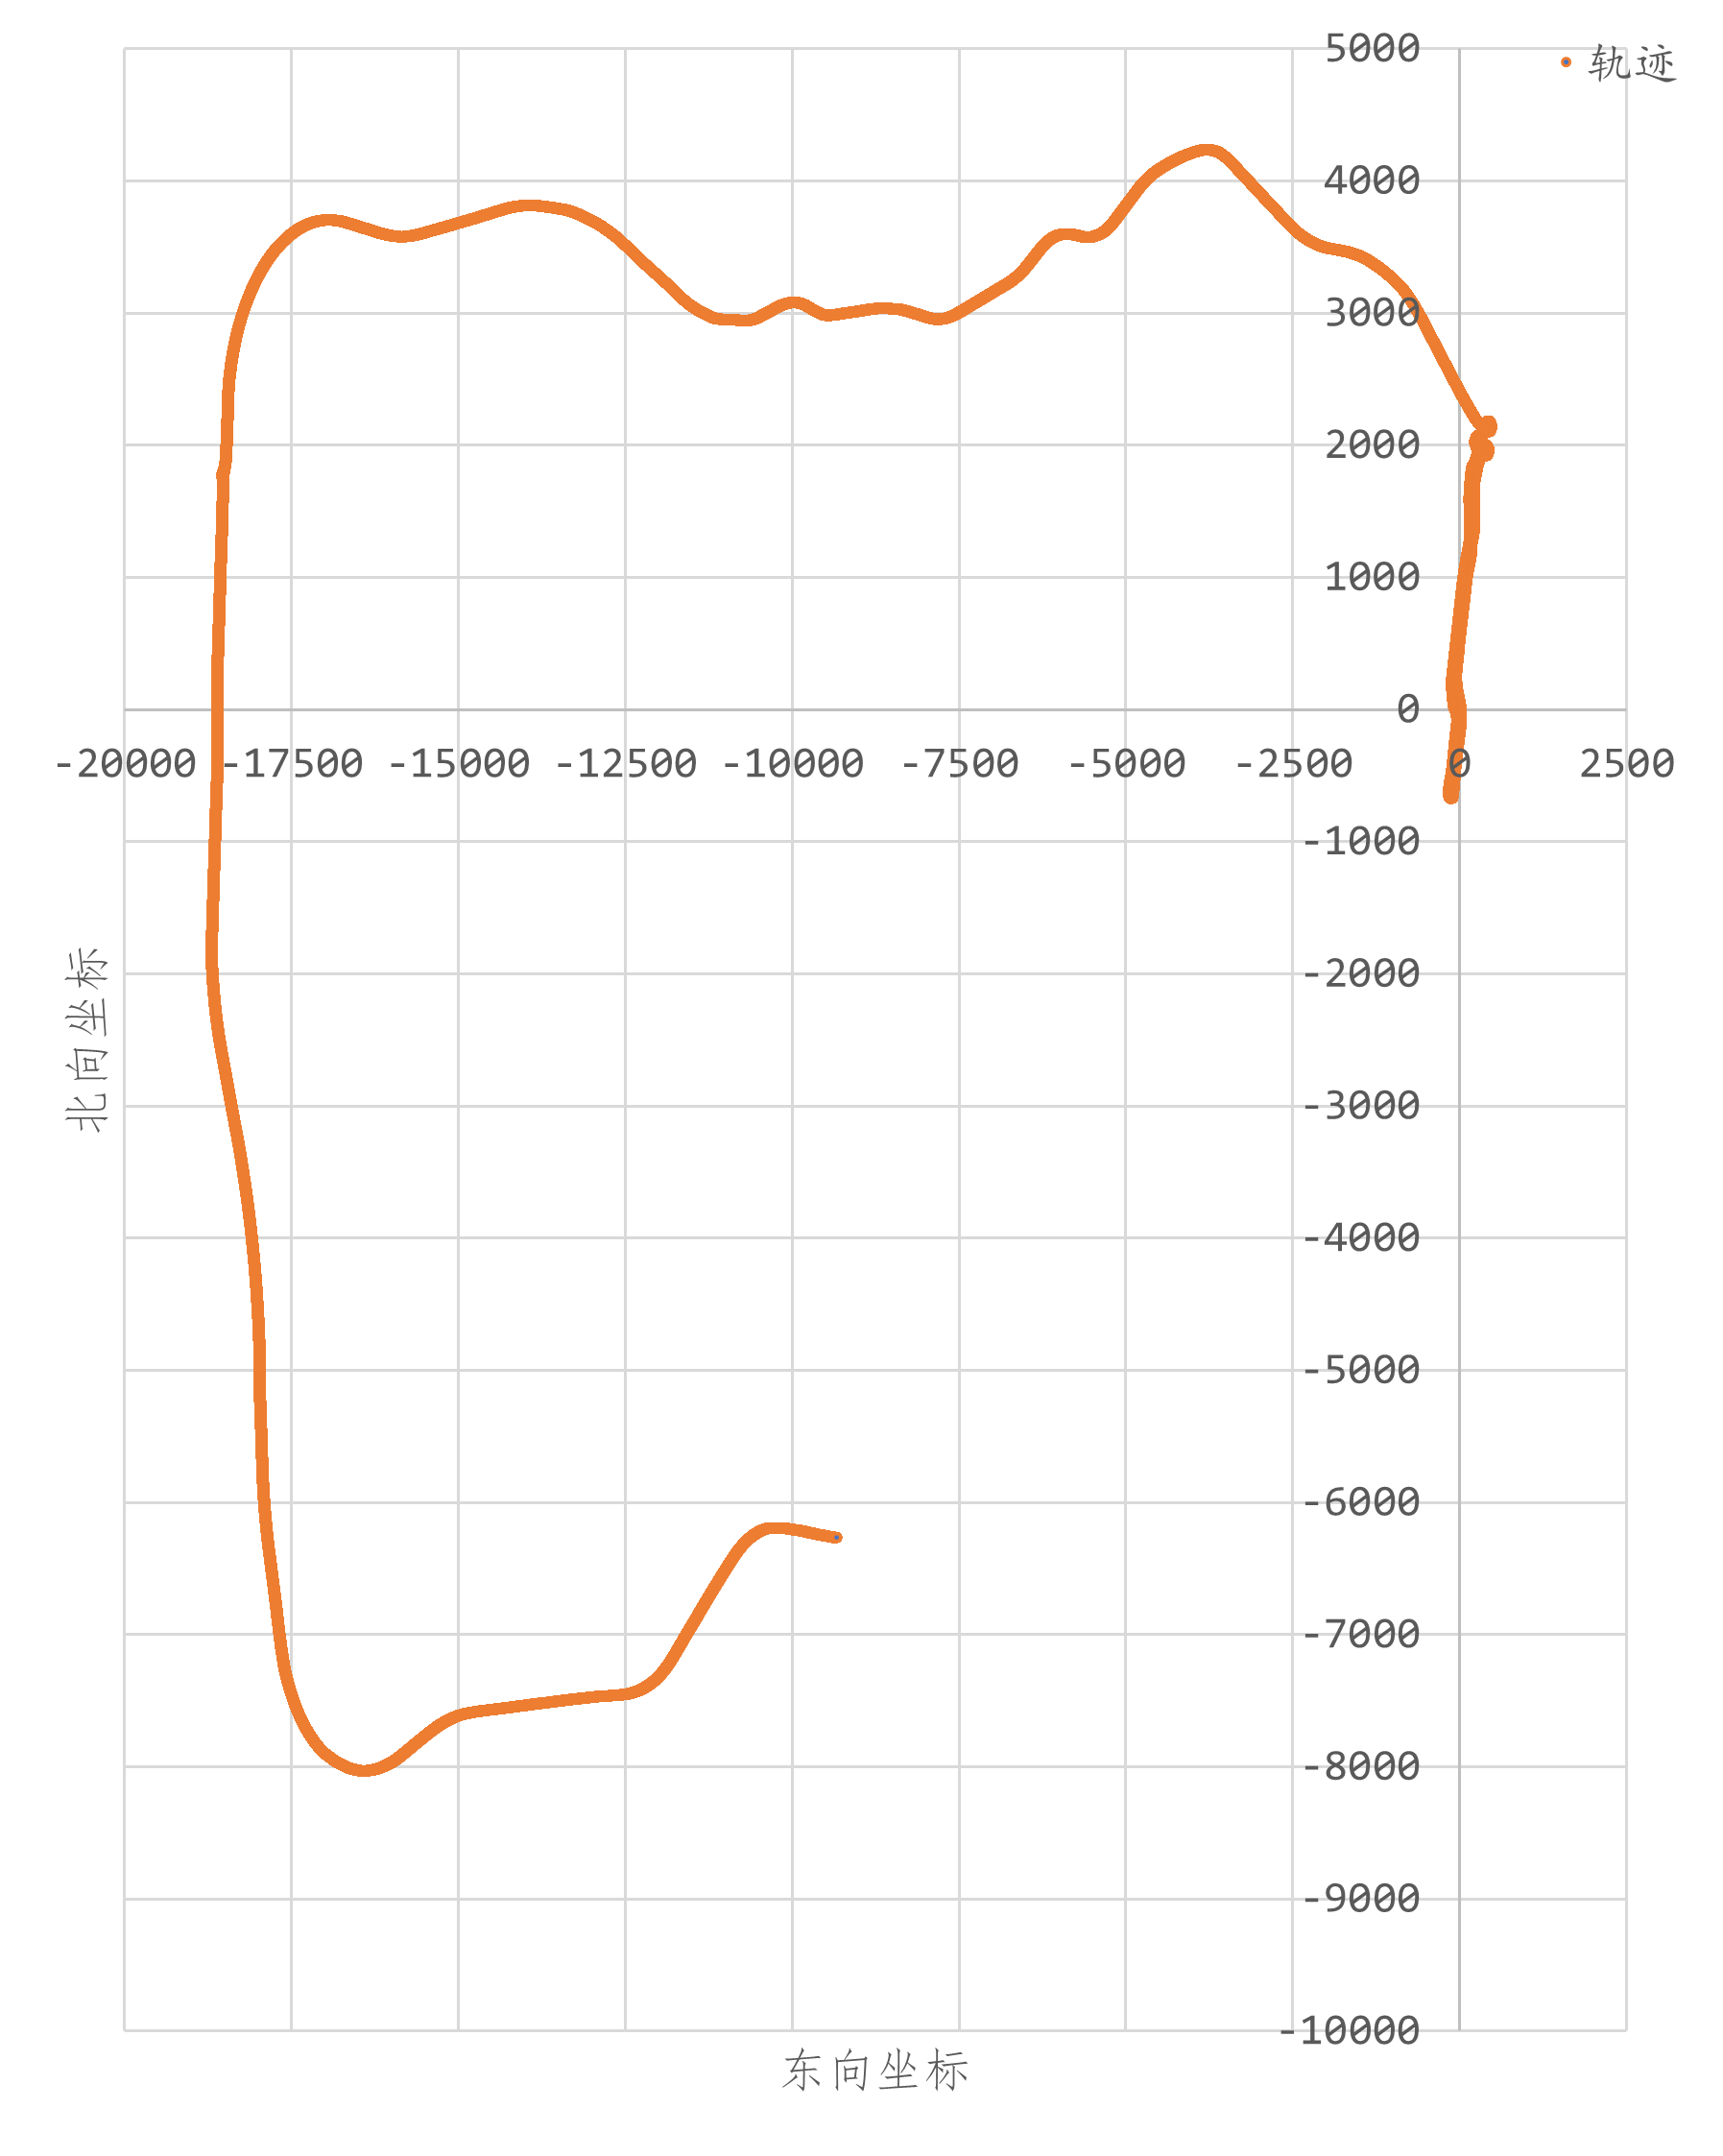
\includegraphics[width=\linewidth]{Figures/DataFigure/示例数据参考结果轨迹.png}
            \caption*{参考轨迹}
        \end{subfigure}
    }
    \caption{示例数据与参考结果轨迹}
    \label{fig:5.3}
\end{figure}

\section{实验数据采集及运行结果}

本小组第一次使用的是黄色\textsf{IMU},即表\ref{tab:IMUInfo}中的第一栏,但是由于仪器故障导致数据无效,所以本组统一改为采用梅芷若小组的实验数据,使用表\ref{tab:IMUInfo}中第二栏的\textsf{IMU}.

\begin{table}[H]
\centering
\begin{tblr}{colspec={ccccc},rowspec={Q[m]Q[m]Q[m]Q[m]Q[m]},hline{1,4,Z}={1pt},vline{2-5}={}}
\SetCell[r=3]{m} \textsf{IMU}型号 & \SetCell[c=2]{c} 陀螺 & & \SetCell[c=2]{c} 加速度计 & \\
\hline
& 零偏 & \textsf{ARW} & 零偏 & \textsf{VRW} \\
& (deg/h,1$\sigma$) & (deg/$\sqrt{\mathrm{h}}$) & (mGal,1$\sigma$) & (m/s/$\sqrt{\mathrm{h}}$) \\
{星宇网达\\ \textsf{XW-7681}} & 0.05(bias) & 0.01 & 30(bias) & 0.03 \\
\textsf{SPAN-CPT} & {20(bias) \\ 1(bias instability)} & 0.07 & {50000(bias) \\ 750(bias instability)} & 0.1 \\
\end{tblr}
\caption{IMU信息}
\label{tab:IMUInfo}
\end{table}

记陀螺仪的航向对准的标准差为$\sigma_{\delta A}$,有
\[
    \sigma_{\delta A} =\frac{\textsf{ARW}}{\omega_e \cos\varphi\sqrt{t}}.
\]
地球自转角速度$\omega_e\approx 15\degree/\mathrm{h}$,当地纬度约$30.5\degree$,初始对准时长均为5min.容易算出
\[
    \sigma_{\delta A_1} \approx 2.7\mathrm{mrad},\sigma_{\delta A_2} \approx 18.7\mathrm{mrad}.
\]

\begin{figure}[H]
    \centering
    {
        \captionsetup{textfont={footnotesize,tt}}
        \begin{subfigure}{0.49\textwidth}
            \centering
            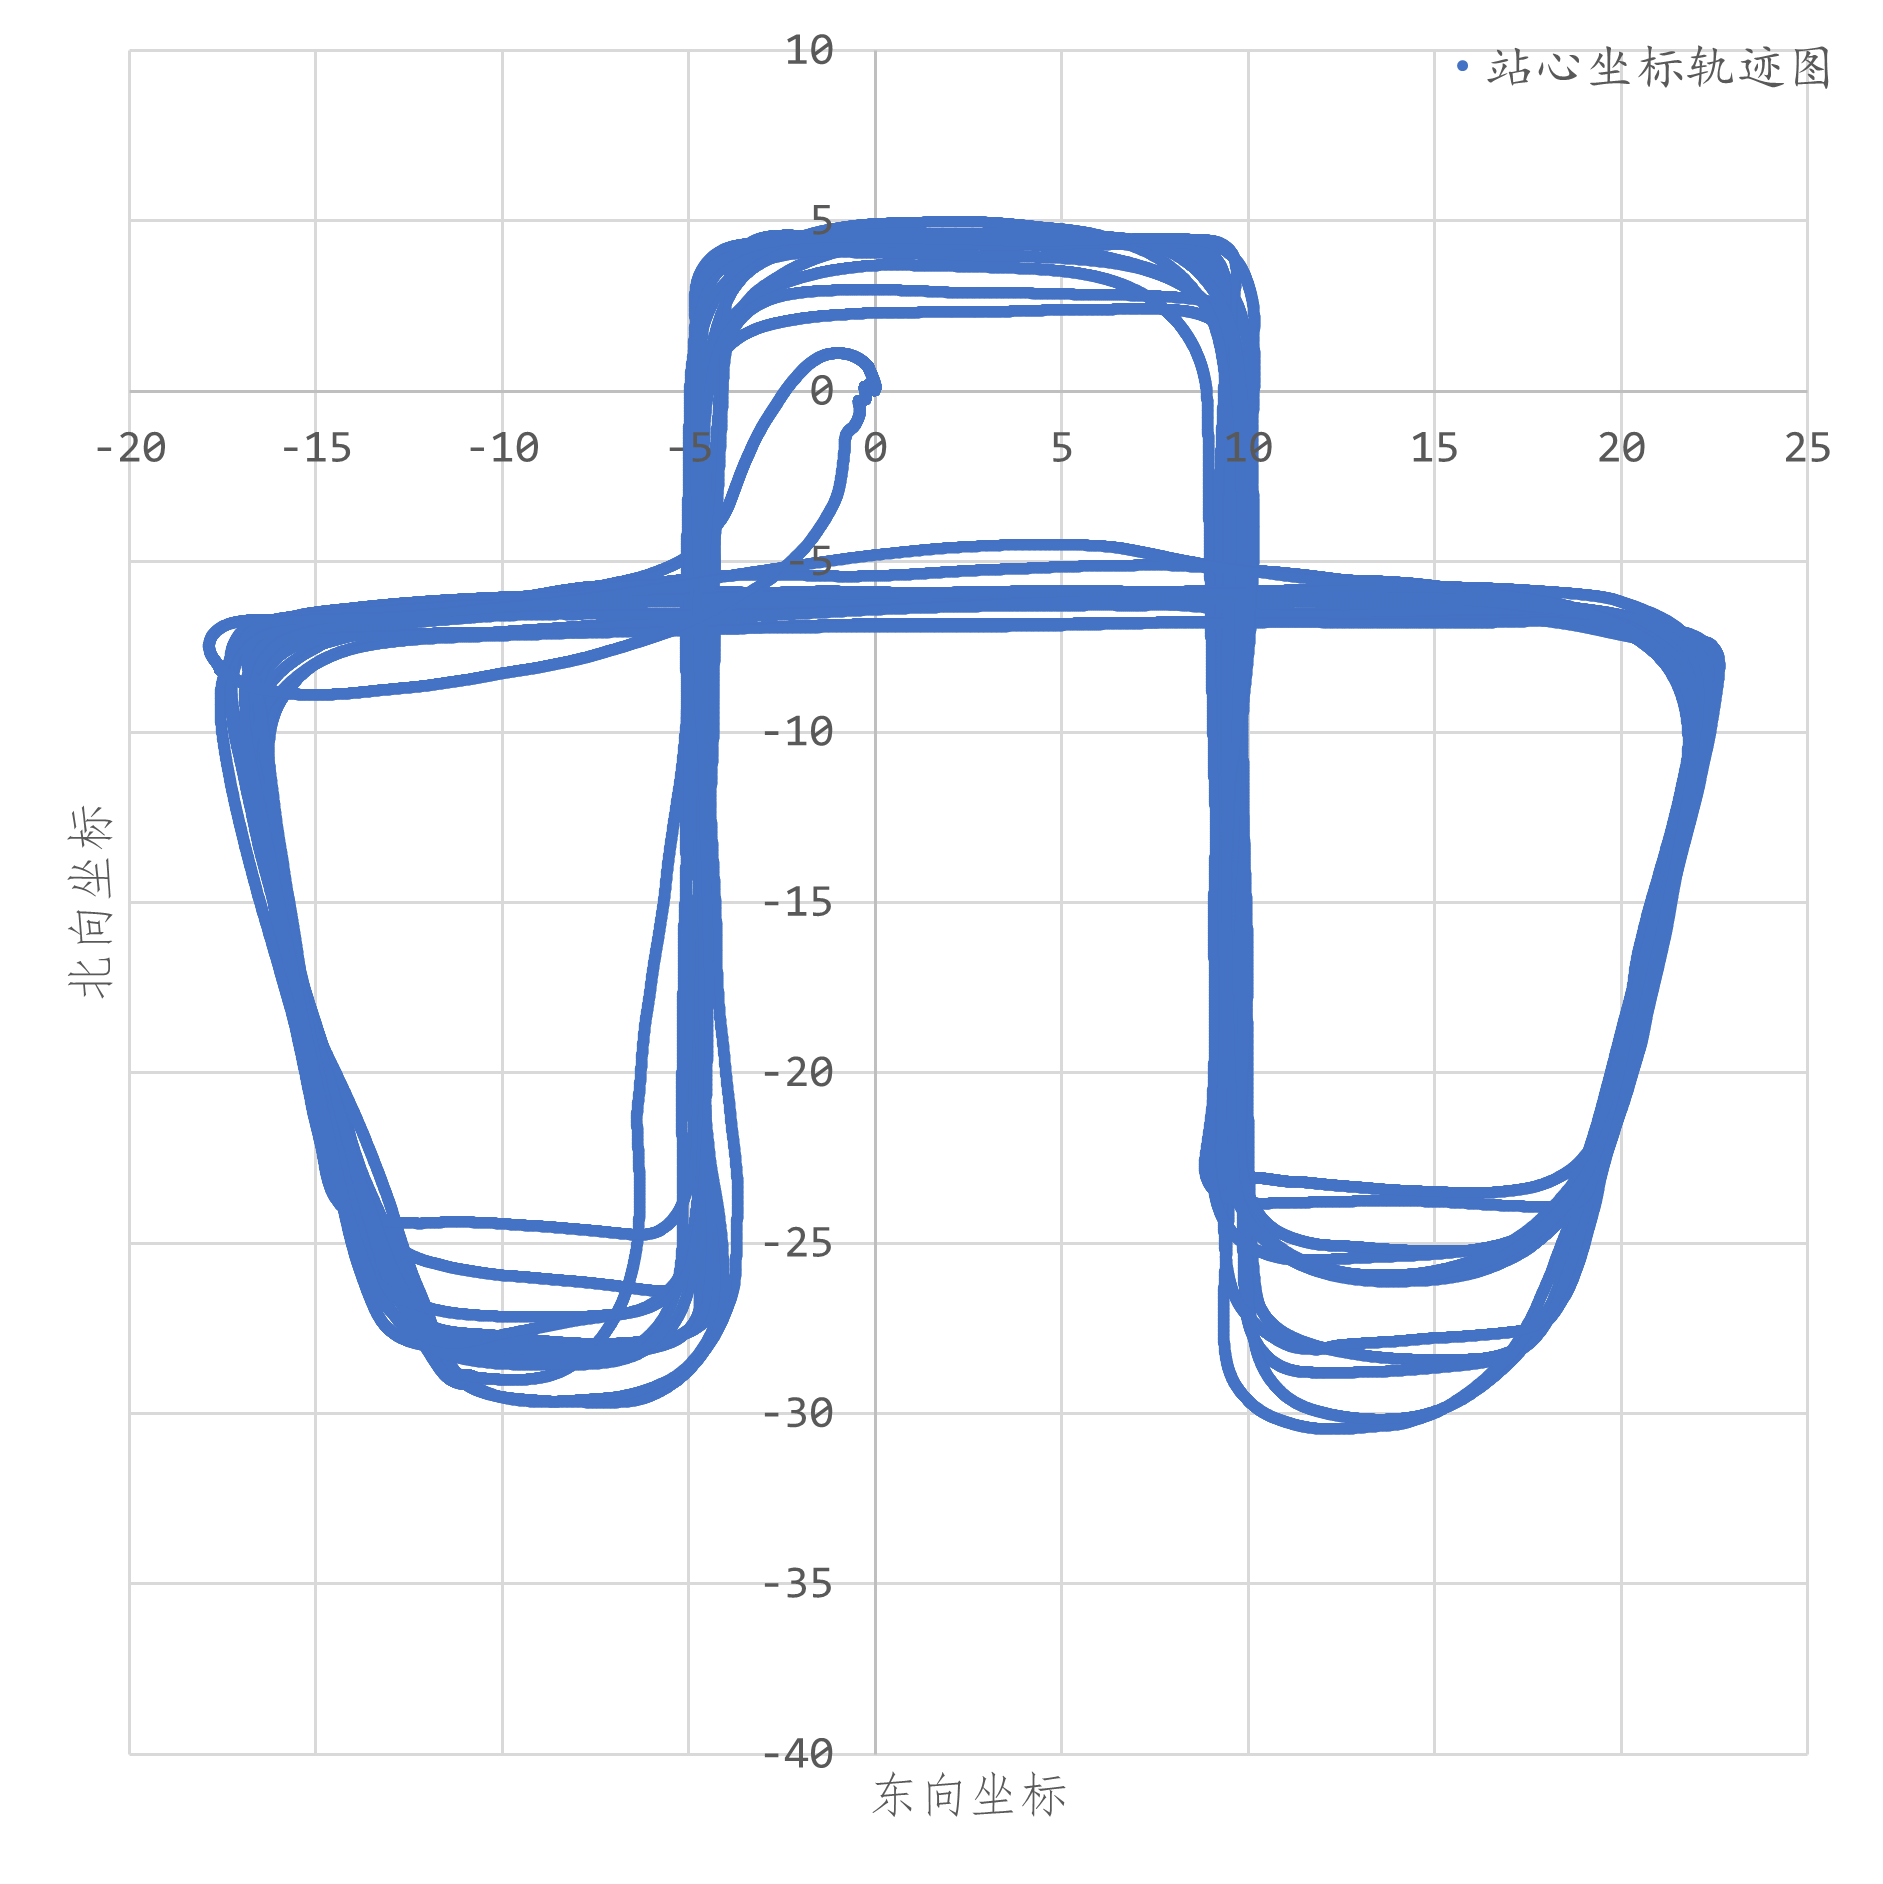
\includegraphics[width=\linewidth]{Figures/DataFigure/品字参考轨迹.png}
            \caption*{\textrm{``}品\textrm{''}\hspace{0mm}字轨迹}
        \end{subfigure}\hfill
        \begin{subfigure}{0.49\textwidth}
            \centering
            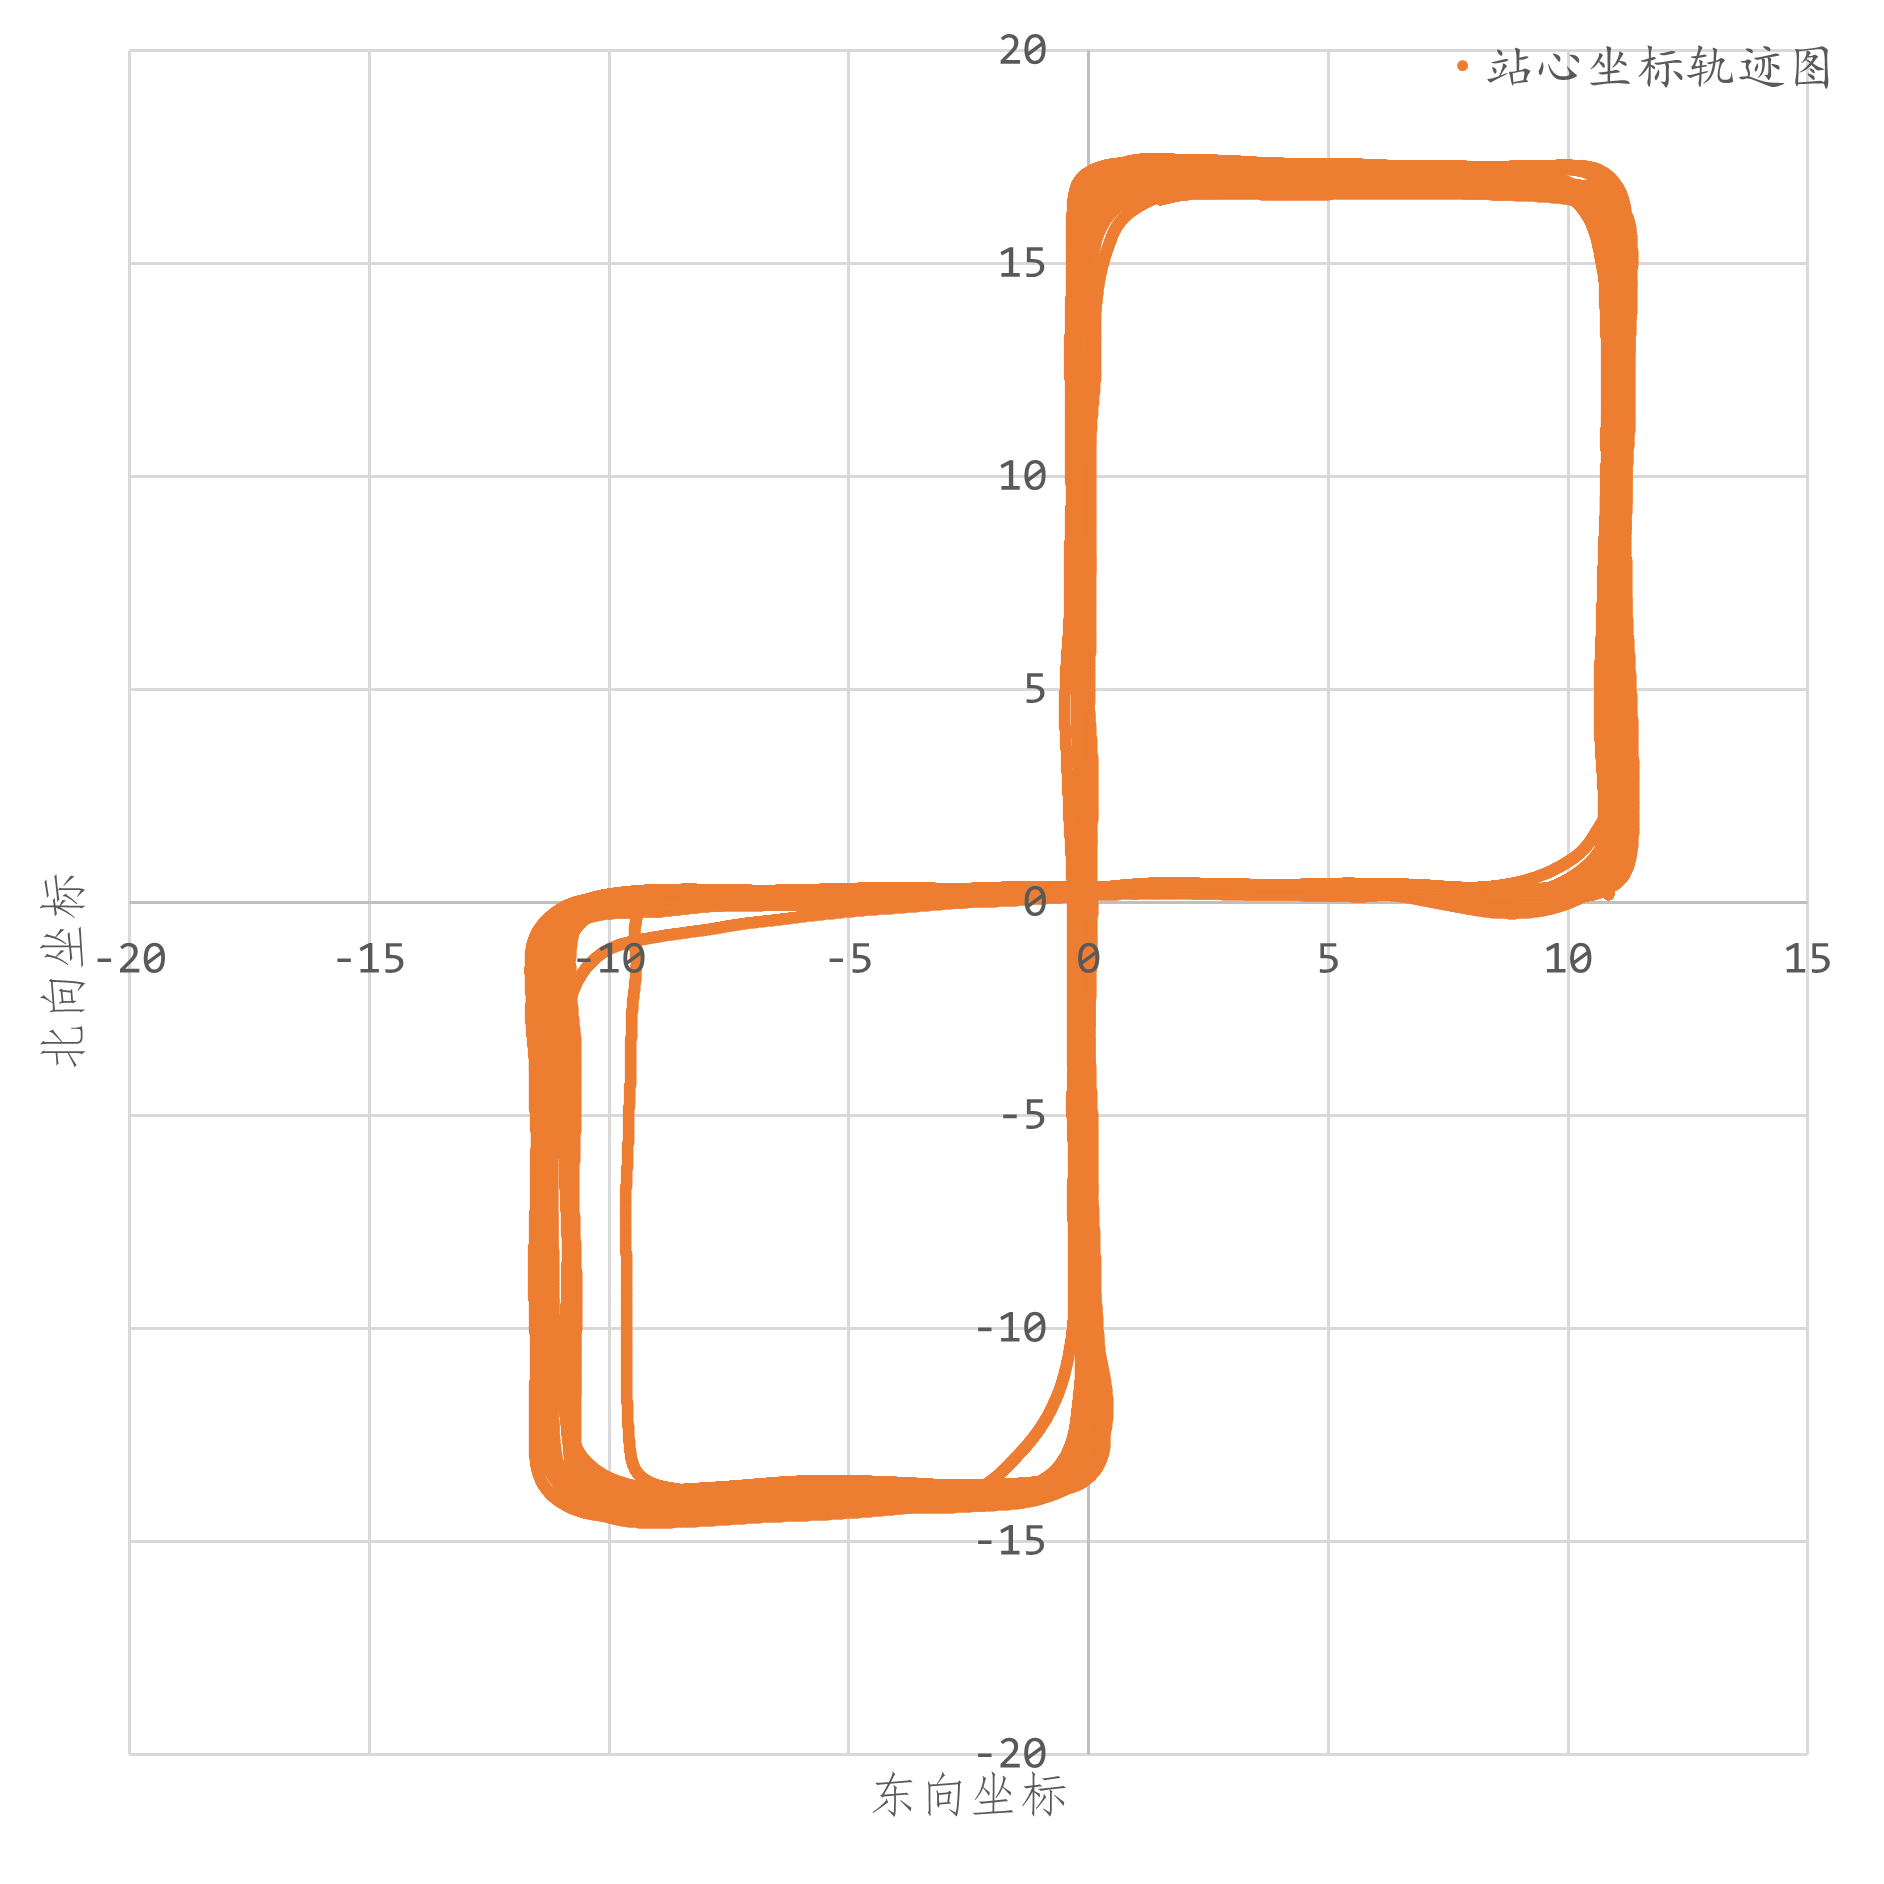
\includegraphics[width=\linewidth]{Figures/DataFigure/8字参考轨迹.png}
            \caption*{\textrm{``}8\textrm{''}\hspace{0mm}字轨迹}
        \end{subfigure}
    }
    \caption{实验运动轨迹}
    \label{fig:6.1}
\end{figure}
如图\ref{fig:6.1}所示,``品''字轨迹是使用星宇网达\textsf{XW-7681}时的运动轨迹,由于\IMU 数据故障,所以只能根据参考结果(\textsf{GNSS}定位)画出轨迹图; ``8''字轨迹是后续数据处理采用数据(即梅芷若小组数据).实验开始前测量的\textsf{GNSS}天线杆臂信息(即接收机相对于\IMU 的坐标)为$(-0.045,0.199,-0.851)$.随后按照\ref{subsec:3.2}节的步骤进行运动.经过五分钟的初始对准,得出开始运动之前的状态为
\begin{description}[nosep]
    \item[初始时间:] \texttt{450799.950}\,s;
    \item[初始位置:] 北纬$\texttt{30.527924682}^{\circ}$,东经$\texttt{114.355680976}^{\circ}$,高\texttt{2.183}m;
    \item[初始速度:] 均为\texttt{0.0}m/s;
    \item[初始姿态:] 横滚角$\texttt{0.12238447}^{\circ}$,俯仰角$\texttt{-0.10672794}^{\circ}$,航向角$\texttt{356.76535600}^{\circ}$.
\end{description}

\subsection{无零速修正}
根据上述数据启动计算,需要注意的是,为了和\textsf{GNSS}数据对齐,第一个历元为\texttt{450501.020}s,所以在保证其他状态相同的情况下,把程序的起算时间记为\texttt{450501.02}s.首先如果不加以零速修正,即对于\ref{subsec:3.2}节中的第(6)步数据不做任何处理,继续采用更新算法计算:
\begin{lstlisting}
//设定初始状态
MotionState startState = new(q0, b0, v0, 450501.02);
//创建ASCData对象,采样率100Hz,数组预分配30万行,不进行零速修正
DataBase data = new ASCData(startState, 0.01, 300000, zeroLambda: null);
//解算并且读取参考数据导出Excel,表名为"实验数据"
data.CalAndExportExcel("ReceivedTofile-COM4-2022_10_21_13-09-37.ASC", "gins.nav", "实验数据");
\end{lstlisting}
生成实验数据的解算结果与参考结果表格用时8.5s.由于未进行零速修正,所以发散非常快,仅仅是第一圈(大约37000个历元)就已经看不出任何轨迹:如图\ref{fig:6.2}所示.零速修正后的前37000个历元是可以看出``8''字形状的,造成这种现象是因为初始状态后静止了5分钟但是\IMU 输出不完全为0,可见这部分如果不人为设置为零速那么误差积累是相当大的.
\begin{figure}[H]
    \centering
    {
        \captionsetup{textfont={footnotesize,tt}}
        \begin{subfigure}{0.49\textwidth}
            \centering
            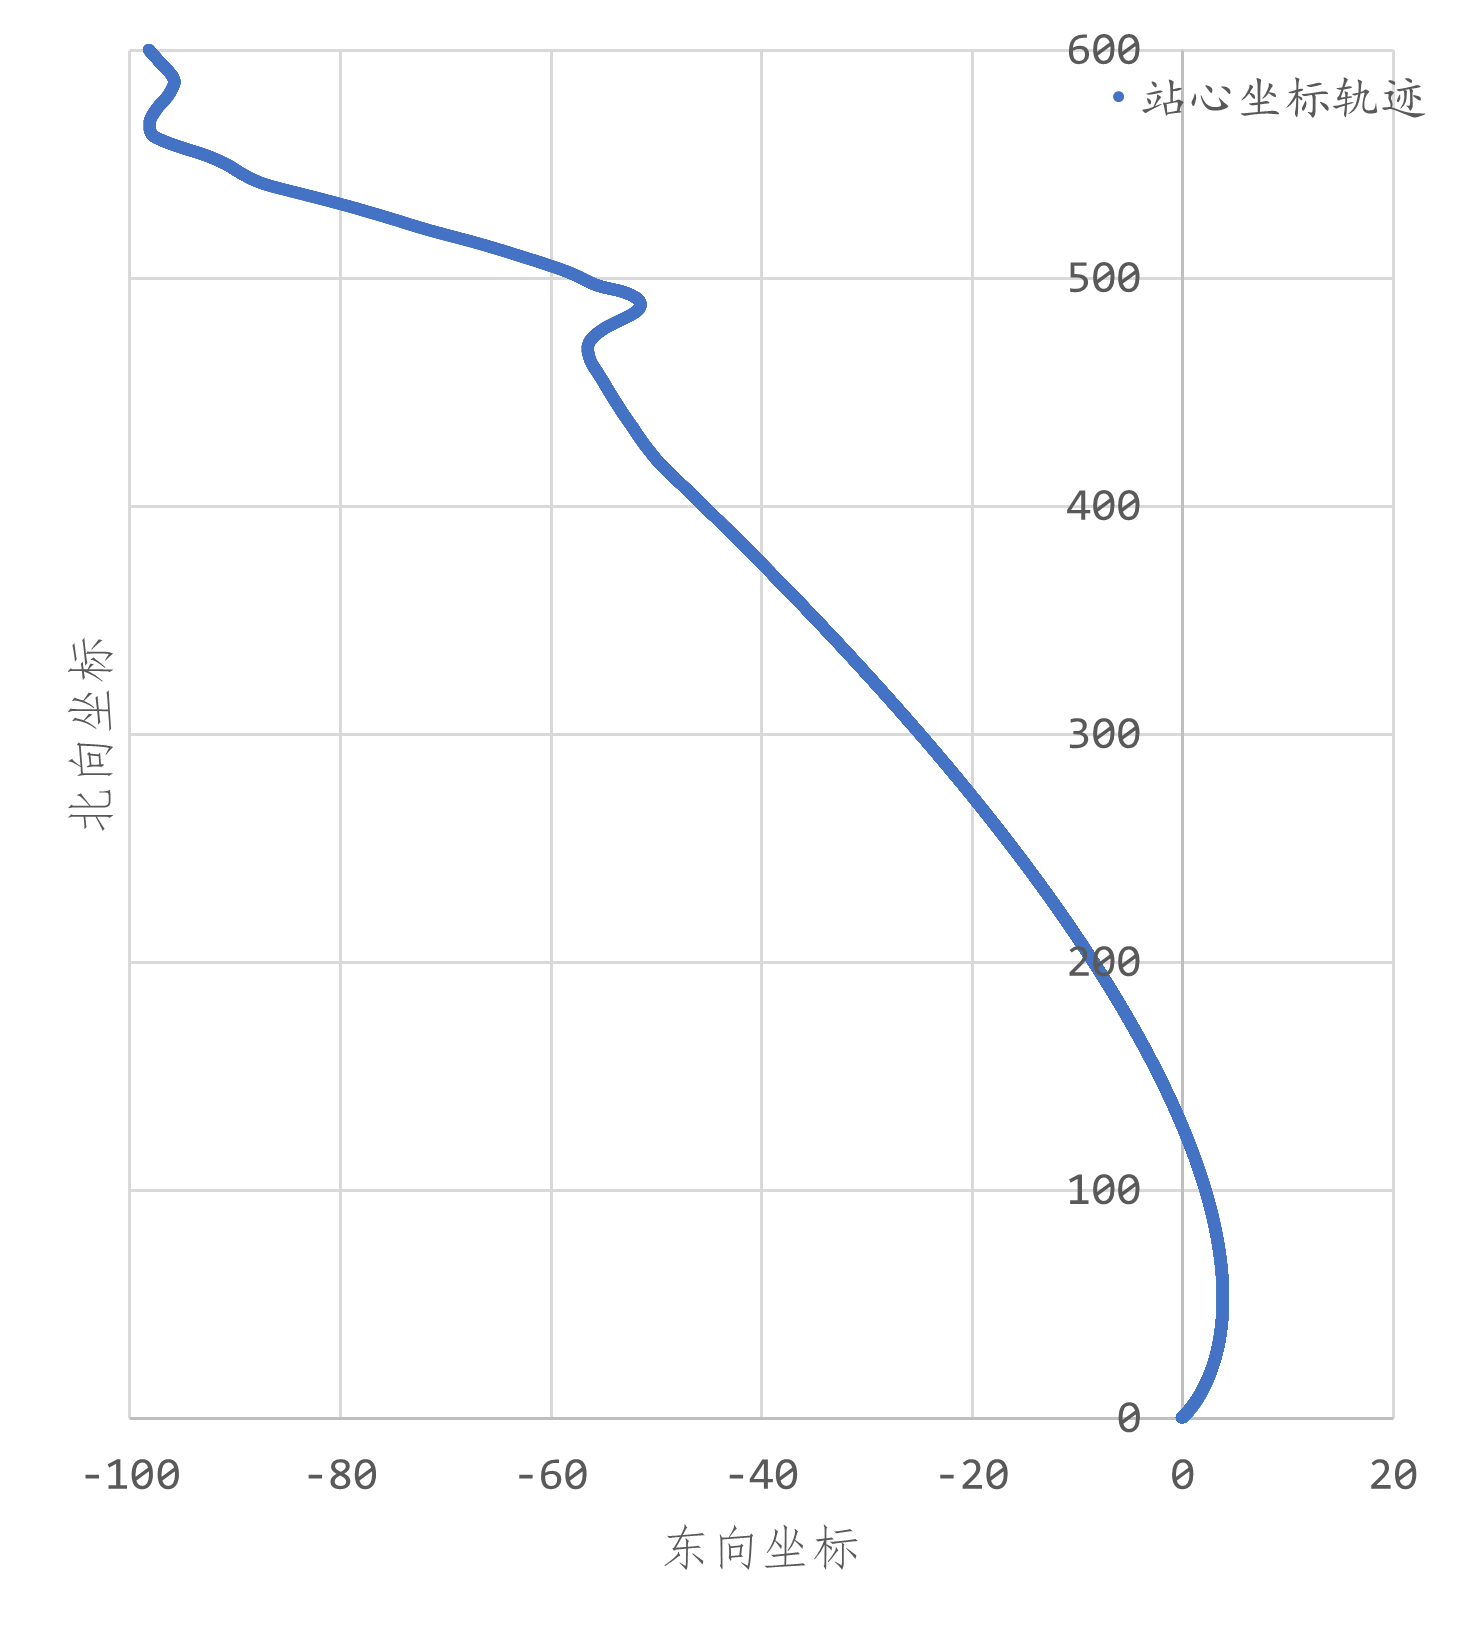
\includegraphics[width=\linewidth]{Figures/DataFigure/无零速修正前37000历元.png}
            \caption{无零速修正轨迹}
        \end{subfigure}\hfill
        \begin{subfigure}{0.49\textwidth}
            \centering
            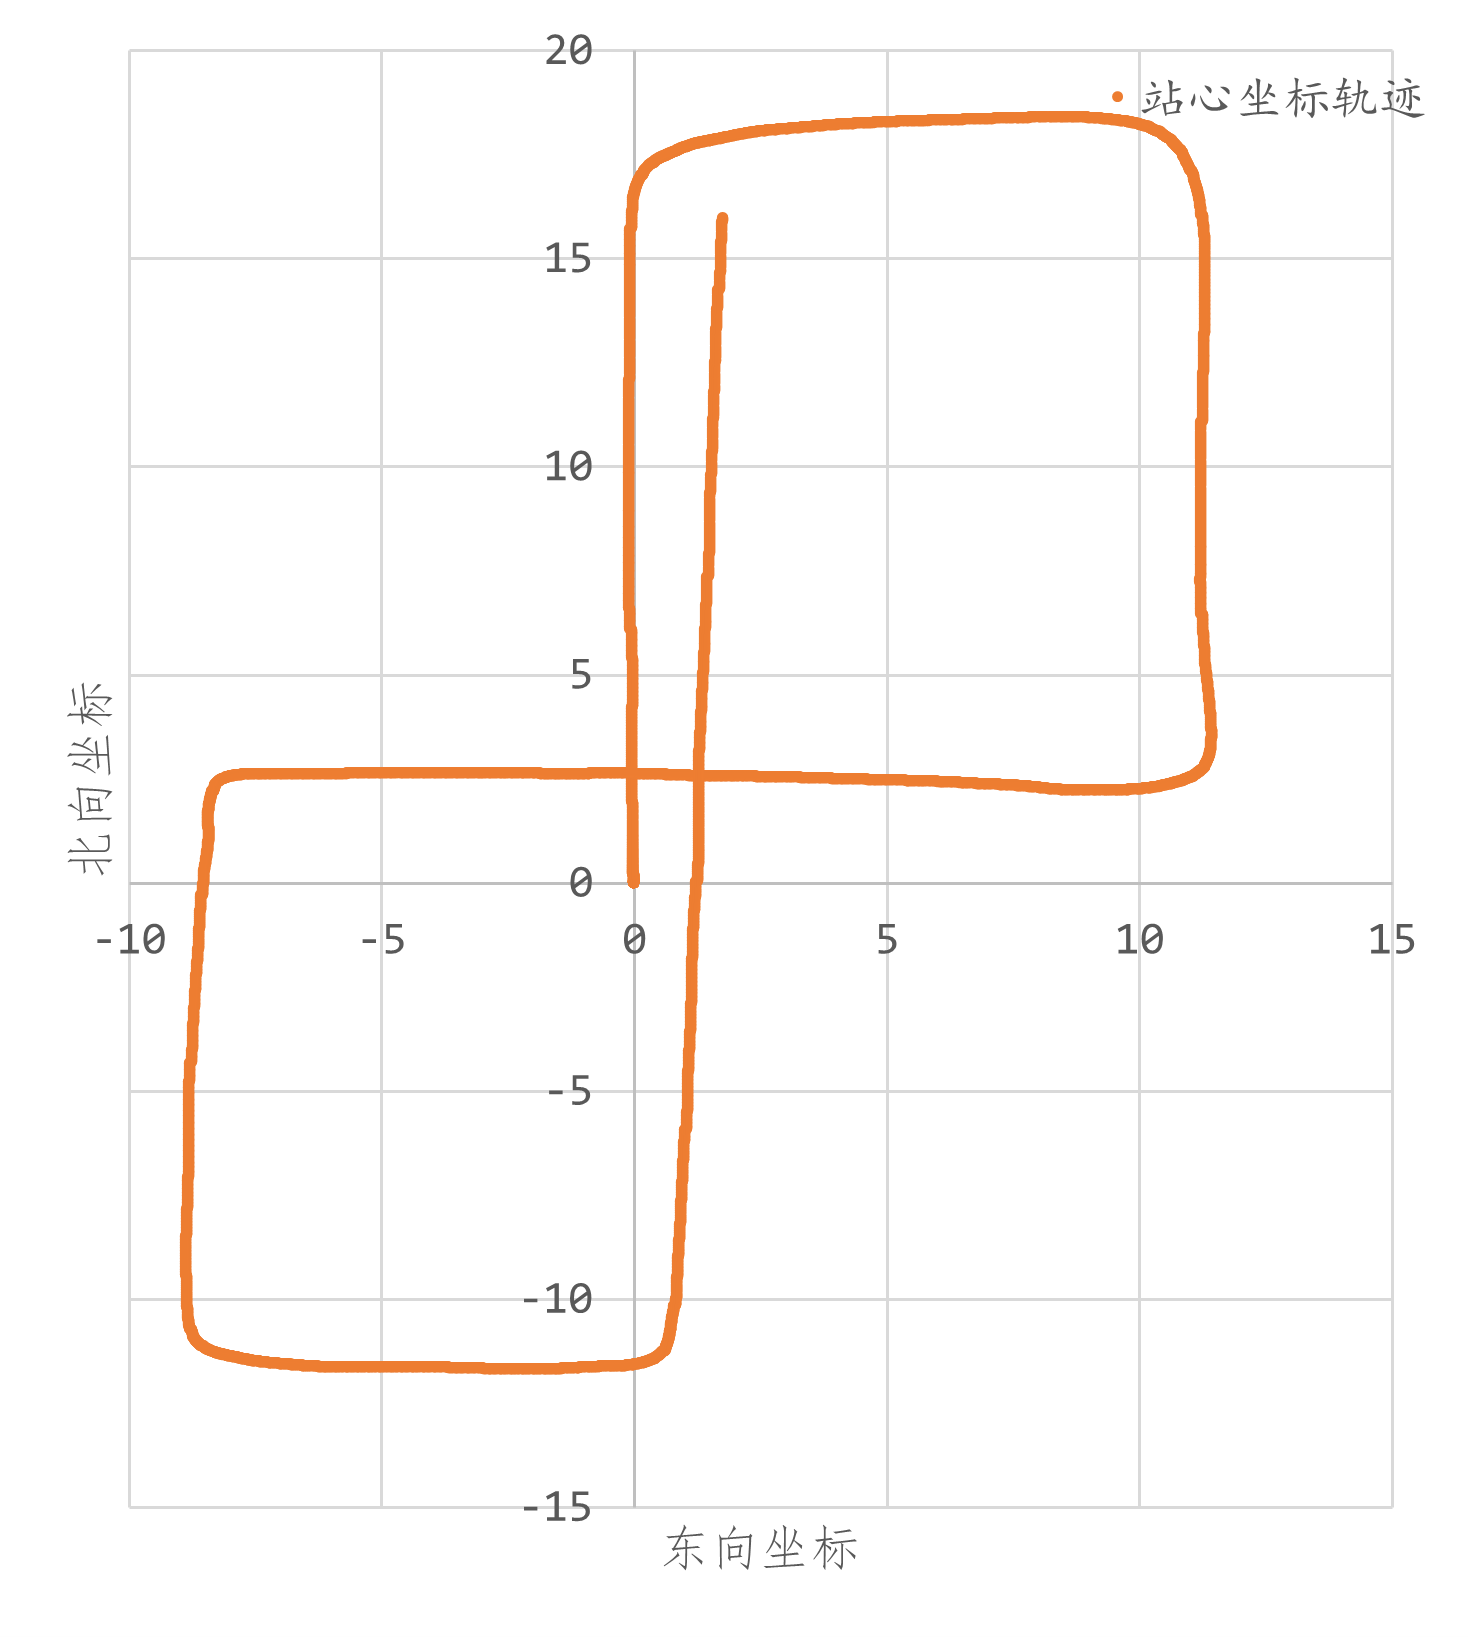
\includegraphics[width=\linewidth]{Figures/DataFigure/零速修正前37000历元.png}
            \caption{零速修正轨迹}
        \end{subfigure}
    }
    \caption{是否零速修正的前37000历元轨迹对比}
    \label{fig:6.2}
\end{figure}
可以预见未零速修正的情况下数据基本上没有参考价值.再来看垂向的数据,如下图所示:
\begin{figure}[H]
    \centering
    {
        \captionsetup{textfont={footnotesize,tt}}
        \begin{subfigure}{0.49\textwidth}
            \centering
            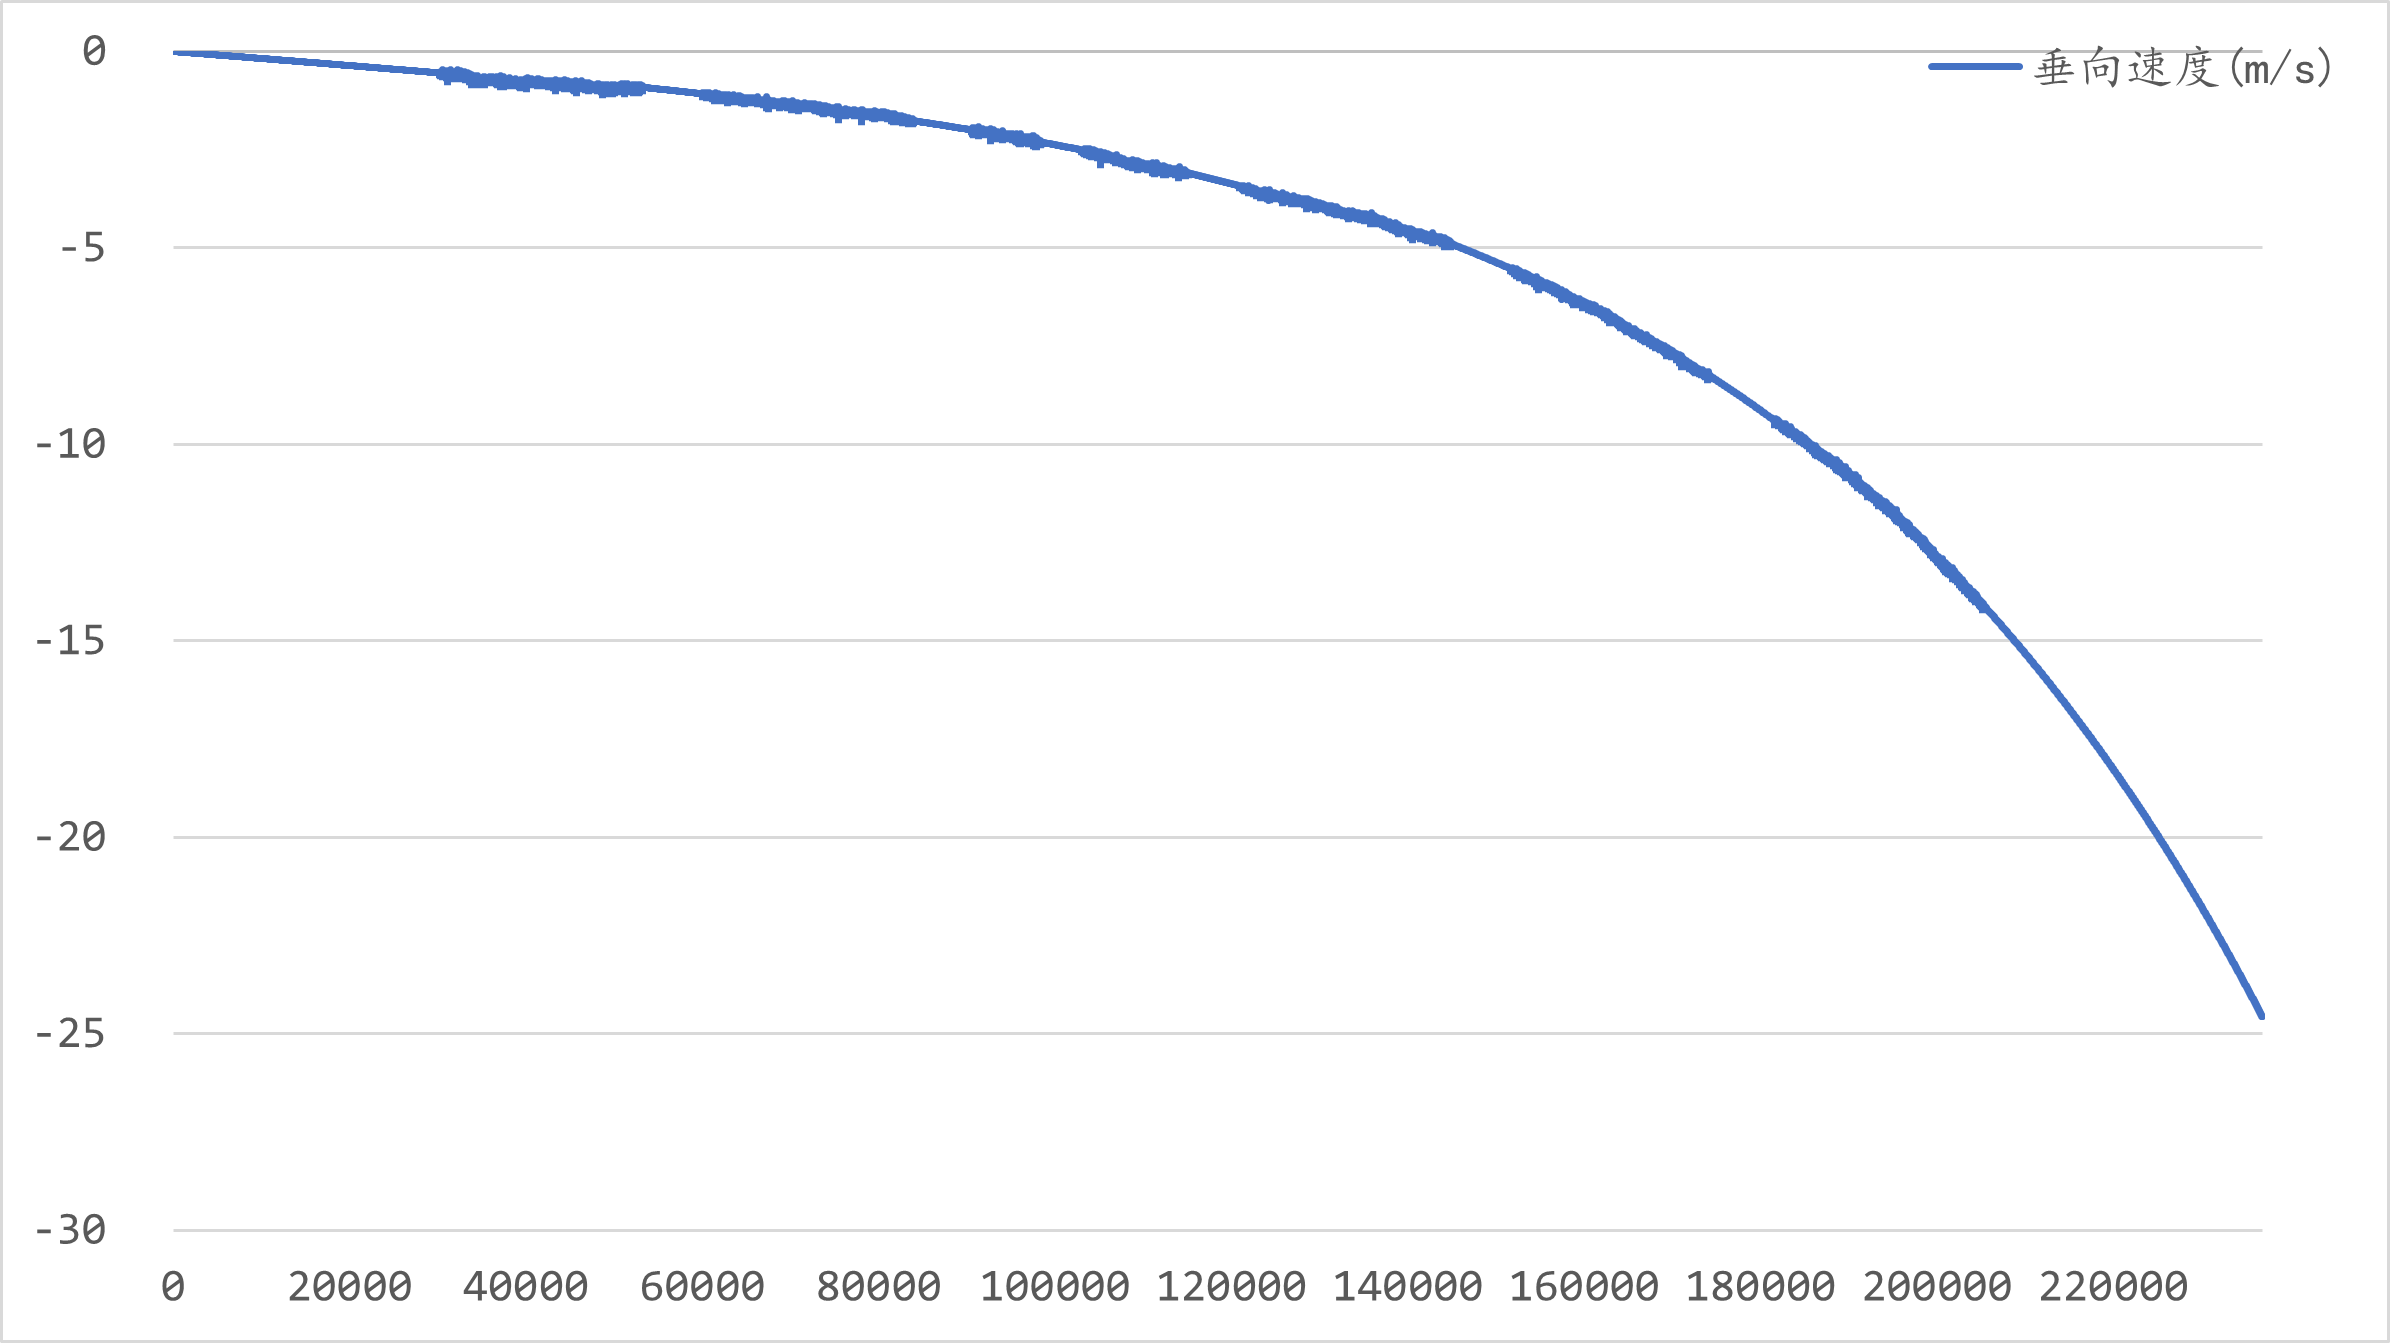
\includegraphics[width=\linewidth]{Figures/DataFigure/未零速修正垂向速度.png}
        \end{subfigure}\hfill
        \begin{subfigure}{0.49\textwidth}
            \centering
            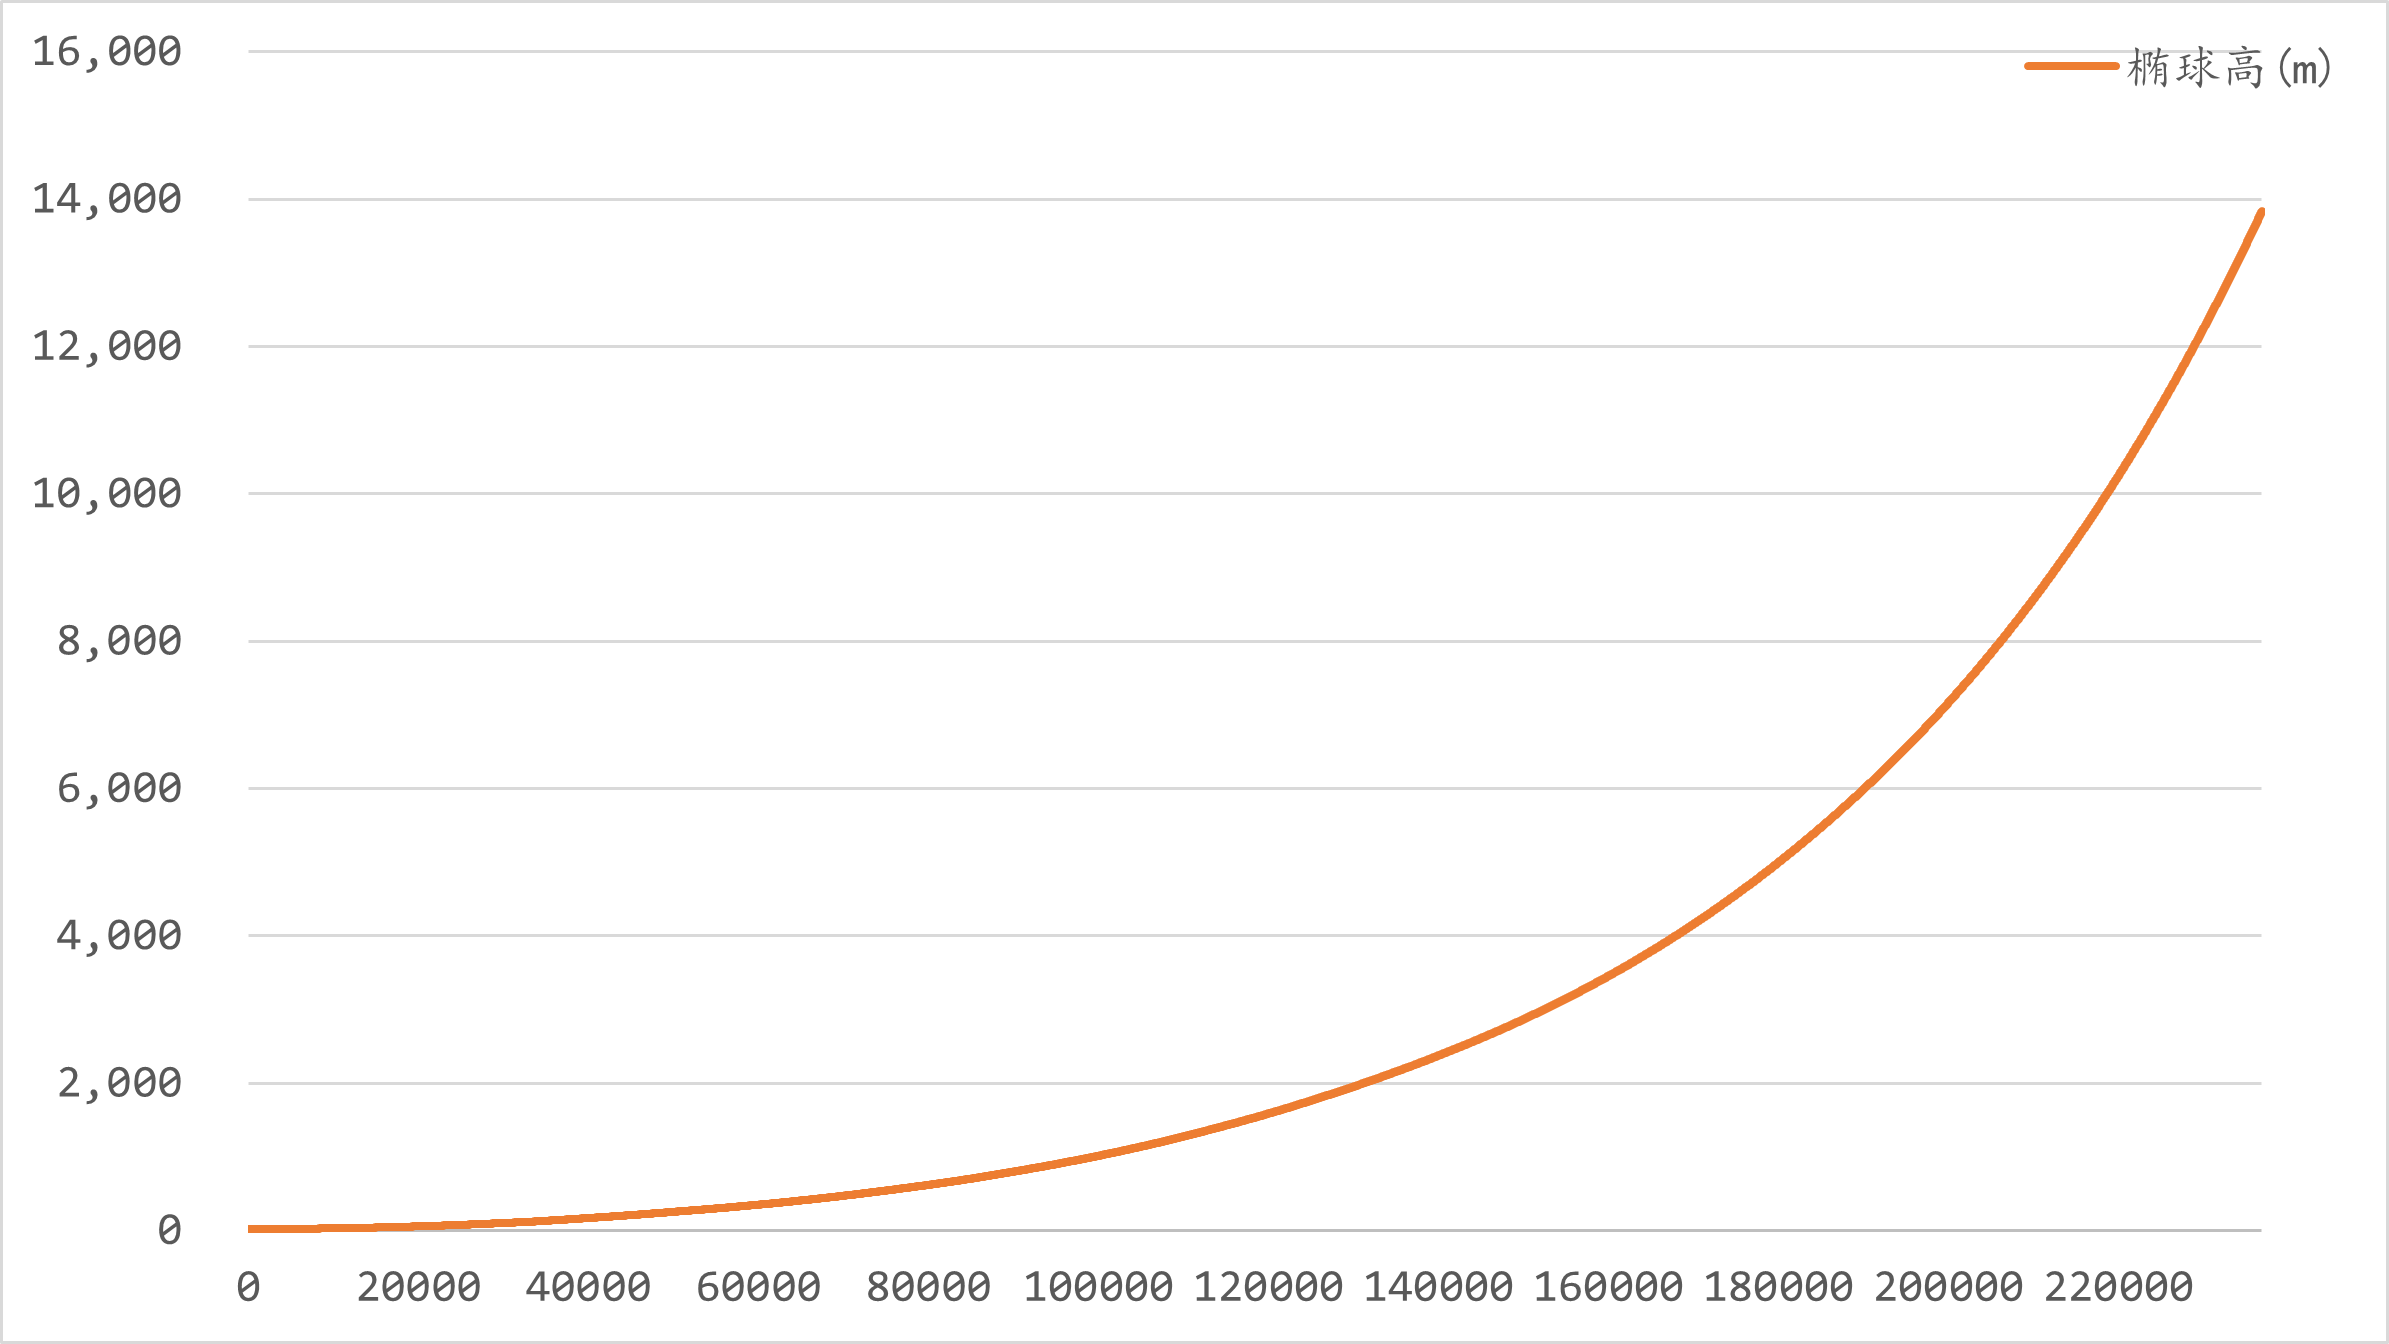
\includegraphics[width=\linewidth]{Figures/DataFigure/未灵素修正高程.png}
        \end{subfigure}
    }
    \caption{未零速修正的垂向数据}
    \label{fig:6.3}
\end{figure}
\noindent 垂向速度$v_D$最后达到了接近$-25\mathrm{m}/\mathrm{s}$,椭球高更是接近$1.4\mathrm{km}$,这进一步表明如果在静止的时候不进行零速修正,由于初始高度误差,初始垂向速度误差,等效垂向加速度计常值零偏和东向速度误差都使得高程误差不断累积,而且根据高程通道的误差分析有:
\begin{equation}\label{eq:6.1}
    \delta h(t) =\delta h_0 \cosh (\sqrt{2} \omega_s t) + \frac{\delta v_{D_0}}{\sqrt{2}\omega_s} \sinh (\sqrt{2}\omega_s t) +
    \frac{2\omega_N \delta v_E -\delta f_D}{2\omega_s^2} \left[ \cosh(\sqrt{2}\omega_s t) - 1 \right] ,
\end{equation}
其中$\omega_s=\sqrt{g/R}$.在长时间静止时,高程误差呈指数发散.而在短时间静止时,例如此次实验的前五分钟,此时$\omega_s t$非常小,故上式可近似为
\begin{equation}\label{eq:6.2}
    \delta h(t) =\delta h_0 +\delta v_{D_0}t + \omega_s \delta h_0 t^2 +\omega_N \delta v_E t^2 - \frac{1}{2}\delta f_D t^2.
\end{equation}
高程误差为垂向加速度计误差的二次函数.

\subsection{零速修正}

初始状态设置与上文相同.采用零速修正启动计算:
\begin{lstlisting}
//设定初始状态
MotionState startState = new(q0, b0, v0, 450501.02);
//定义零速修正区间
Func<double, bool> zeroVelCorrect = time => time < 450799.950 || (time > 451033.64 && time < 451096.48) || (time >451342.26 && time < 451405.06) || (time > 451487.10 && time < 451530.34) || (time > 451652.58 && time < 451710.89) || (time > 451952.42 && time < 452016.83) || (time > 452245.30 && time < 452313.44) || time > 452559.93;
//创建ASCData对象,采样率100Hz,数组预分配30万行,进行零速修正
DataBase data = new ASCData(startState, 0.01, 300000, zeroLambda: zeroVelCorrect);
//解算并且读取参考数据导出Excel,表名为"实验数据"
data.CalAndExportExcel("ReceivedTofile-COM4-2022_10_21_13-09-37.ASC", "gins.nav", "实验数据");
\end{lstlisting}
生成实验数据的解算结果与参考结果表格用时8.5s.将零速修正后的结果前37000个历元的轨迹(图\ref{fig:6.2})和参考结果的轨迹(图\ref{fig:6.1})画在一起得到下图:
\begin{figure}[H]
    \centering
    {
        \captionsetup{textfont={footnotesize,tt}}
        \begin{subfigure}{0.49\textwidth}
            \centering
            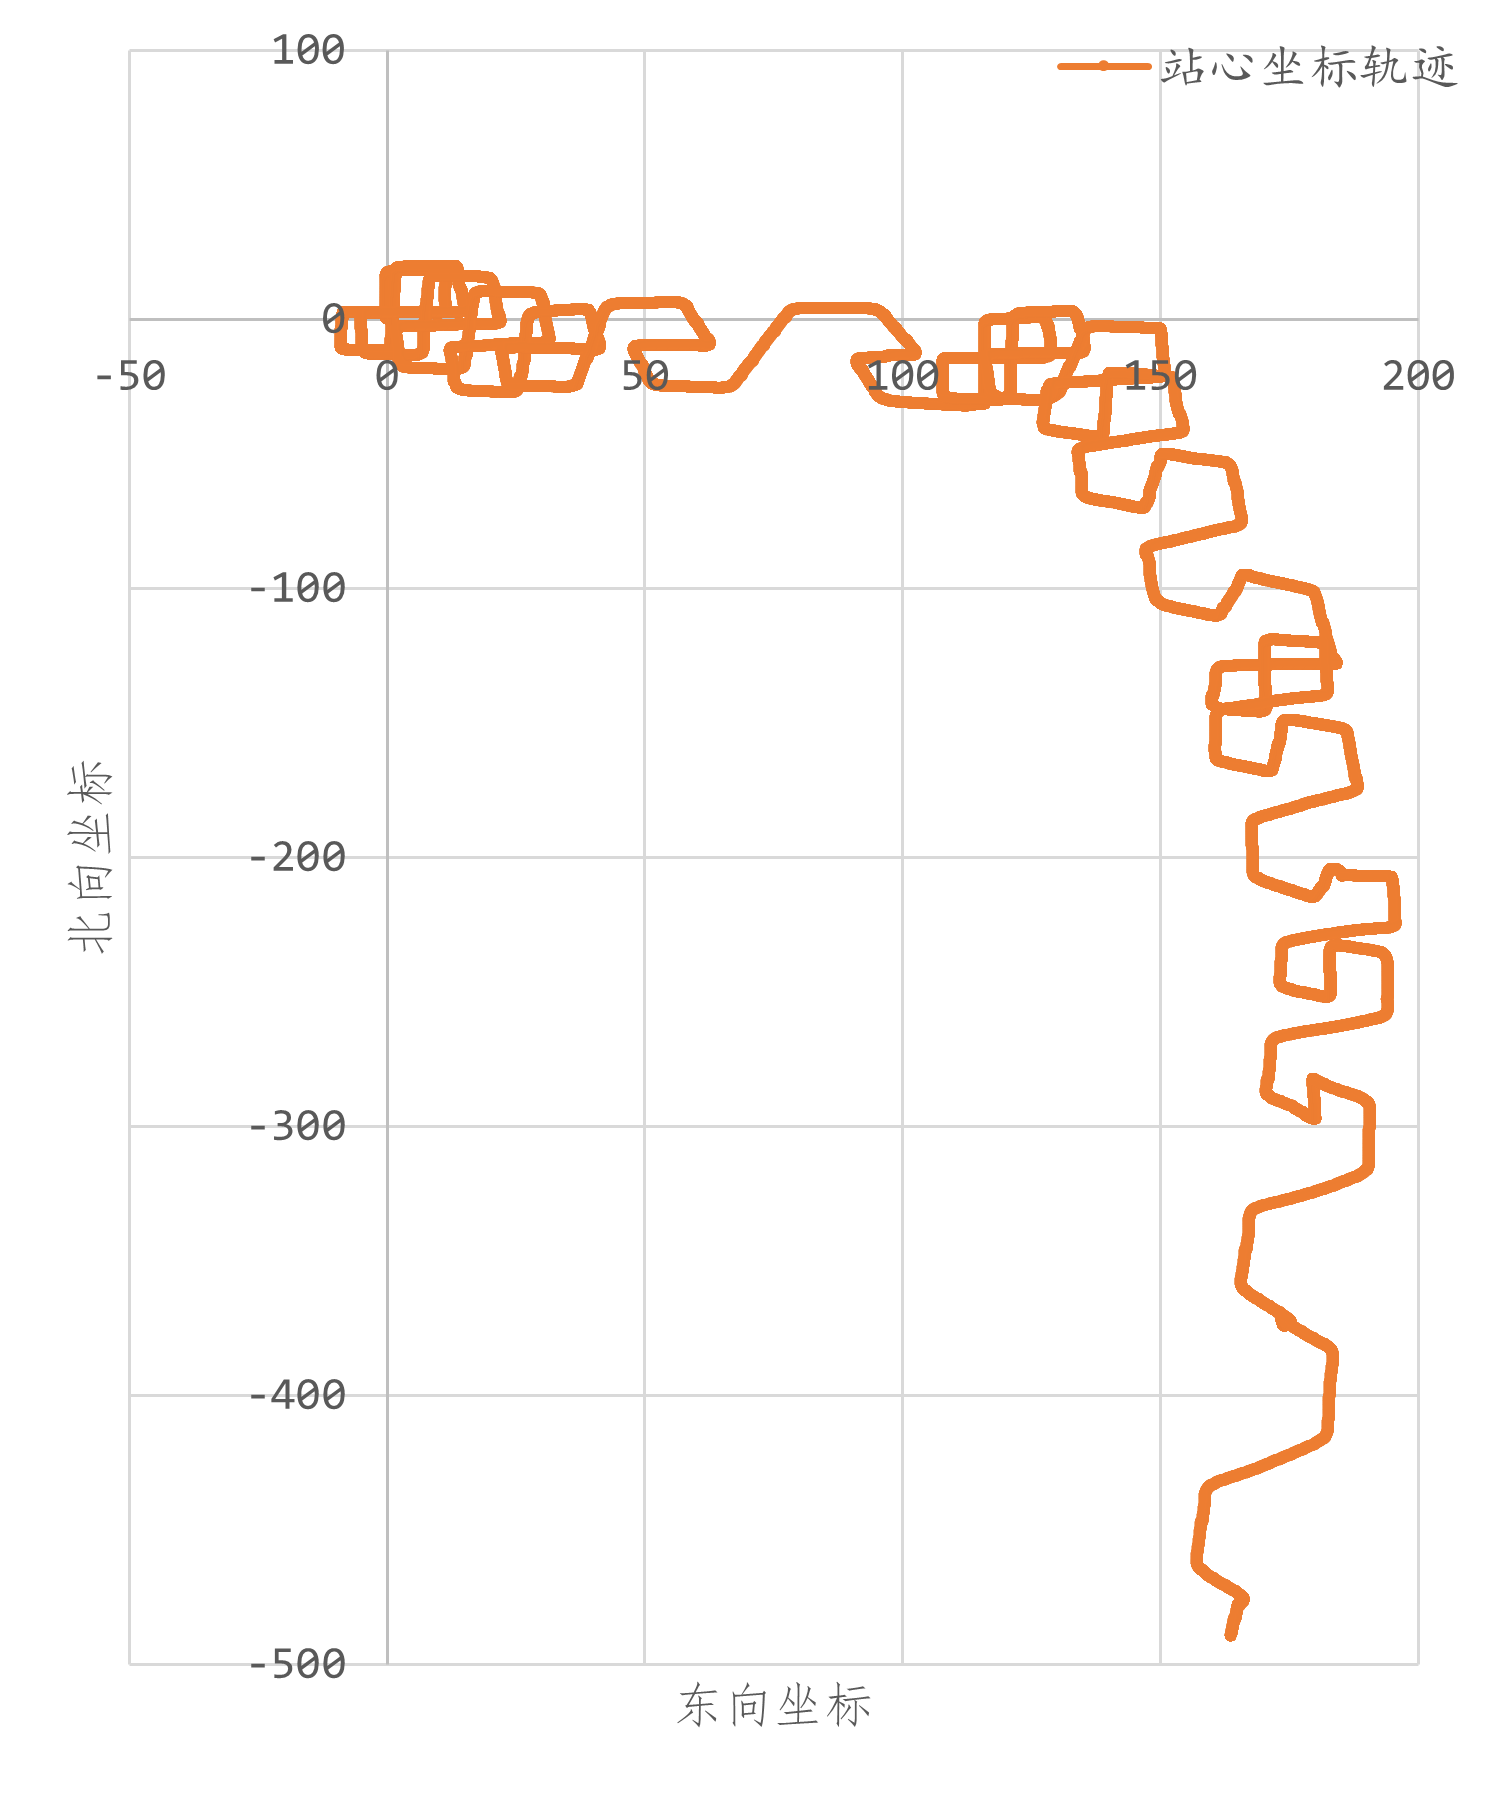
\includegraphics[width=\linewidth]{Figures/DataFigure/灵素修正站心坐标轨迹.png}
            \caption{完整轨迹}
        \end{subfigure}\hfill
        \begin{subfigure}{0.49\textwidth}
            \centering
            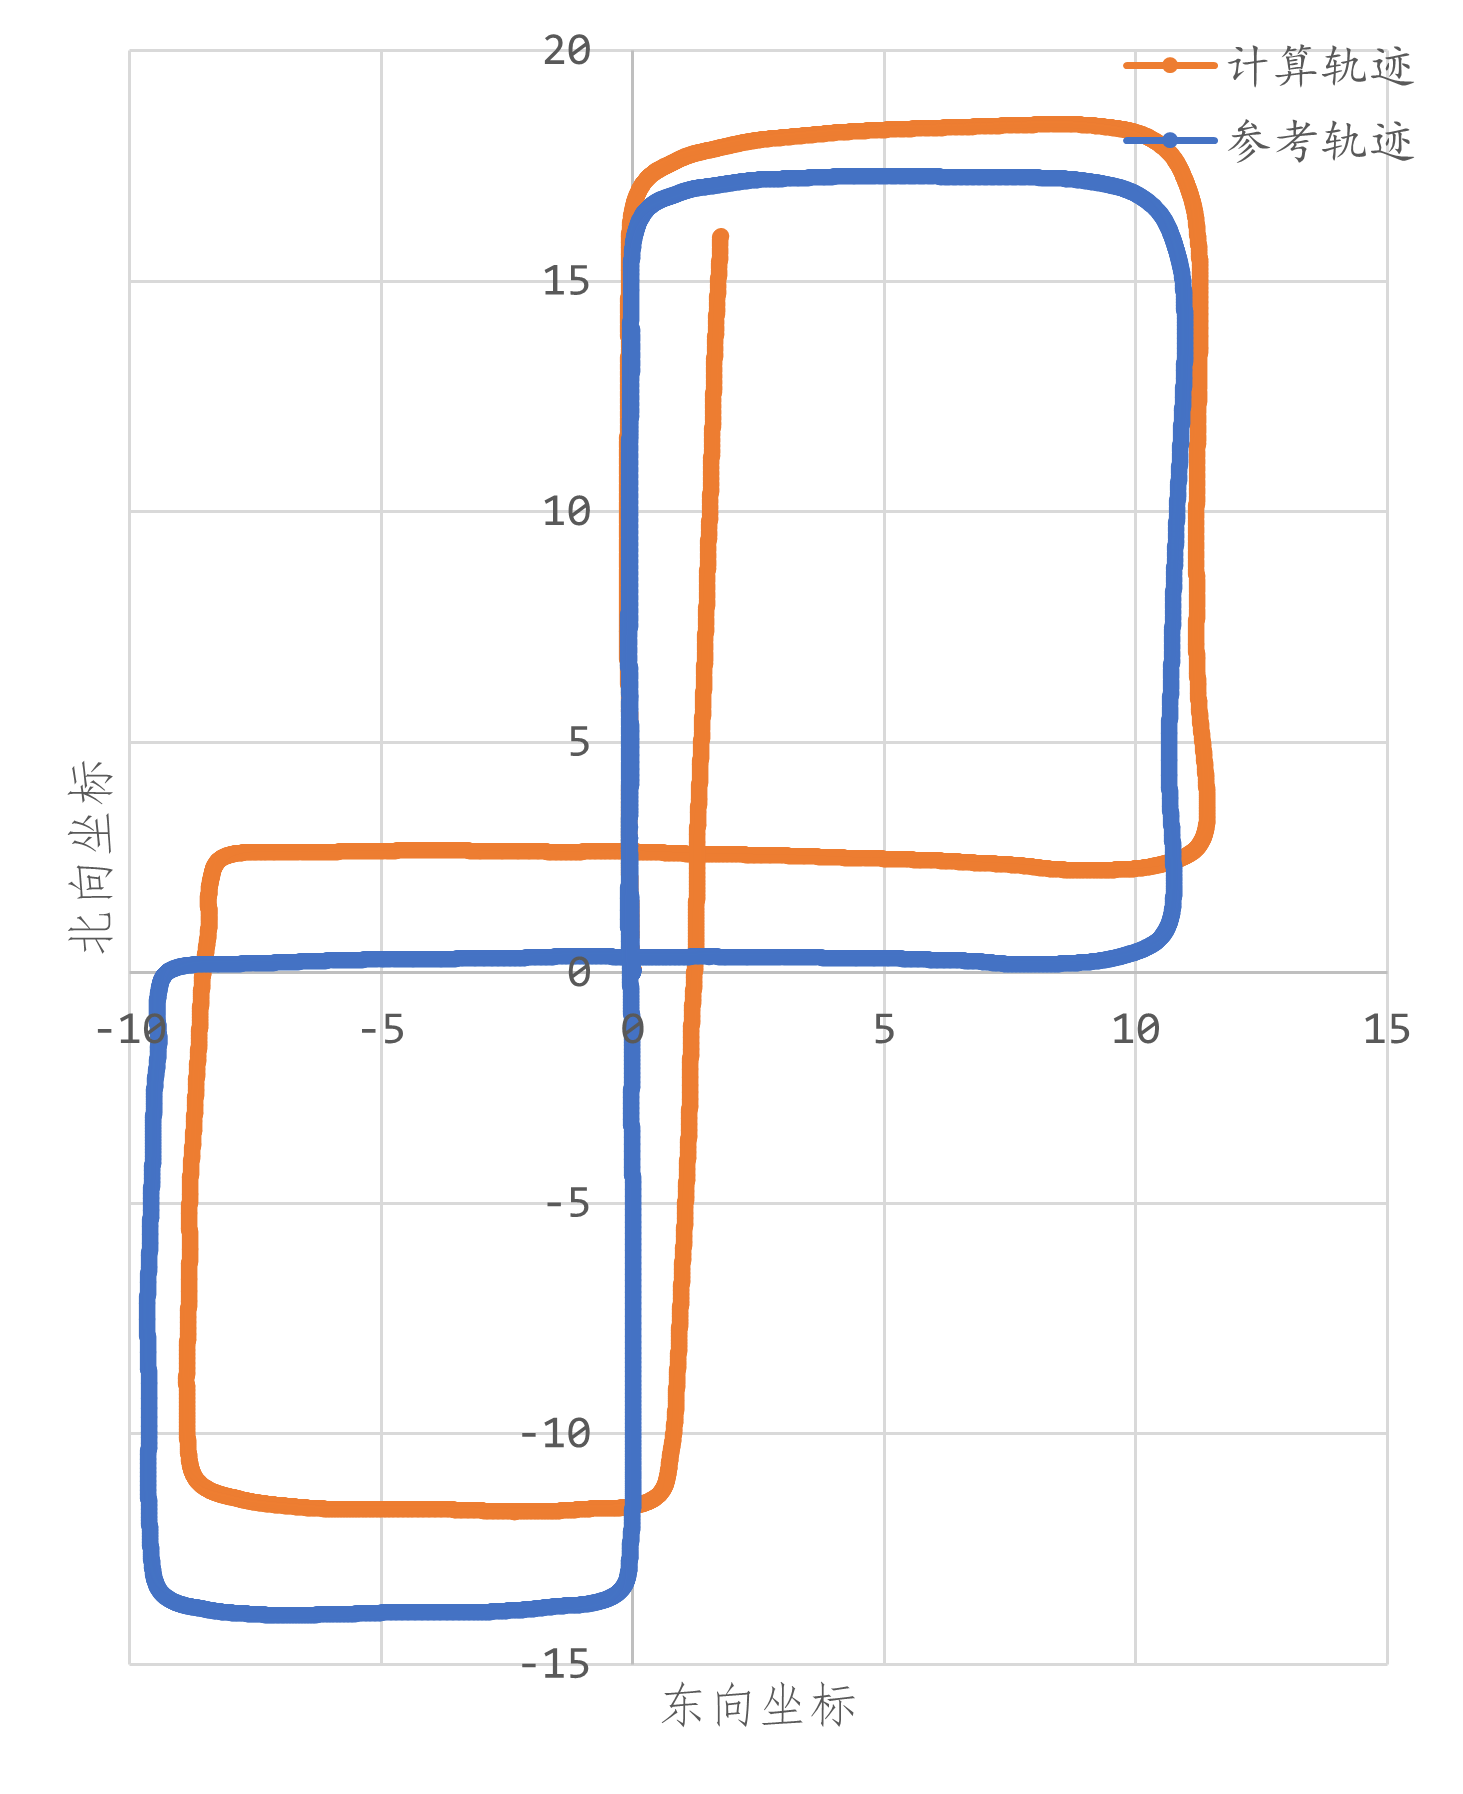
\includegraphics[width=\linewidth]{Figures/DataFigure/灵素修正第一圈轨迹.png}
            \caption{第一圈轨迹}
        \end{subfigure}
    }
    \caption{零速修正轨迹图}
    \label{fig:6.4}
\end{figure}
\noindent 虽然完整轨迹发散依然很严重,但是相比图\ref{fig:6.2},能看出一个个``8''字运动轨迹,并且对于第一圈,虽然和参考轨迹有3--4米的误差,但是能够比较明显的看出``8''字.将其他数据与参考结果做差得到下图:
\begin{figure}[H]
    \centering
    {
        \captionsetup{textfont={footnotesize,tt}}
        \begin{subfigure}{0.49\textwidth}
            \centering
            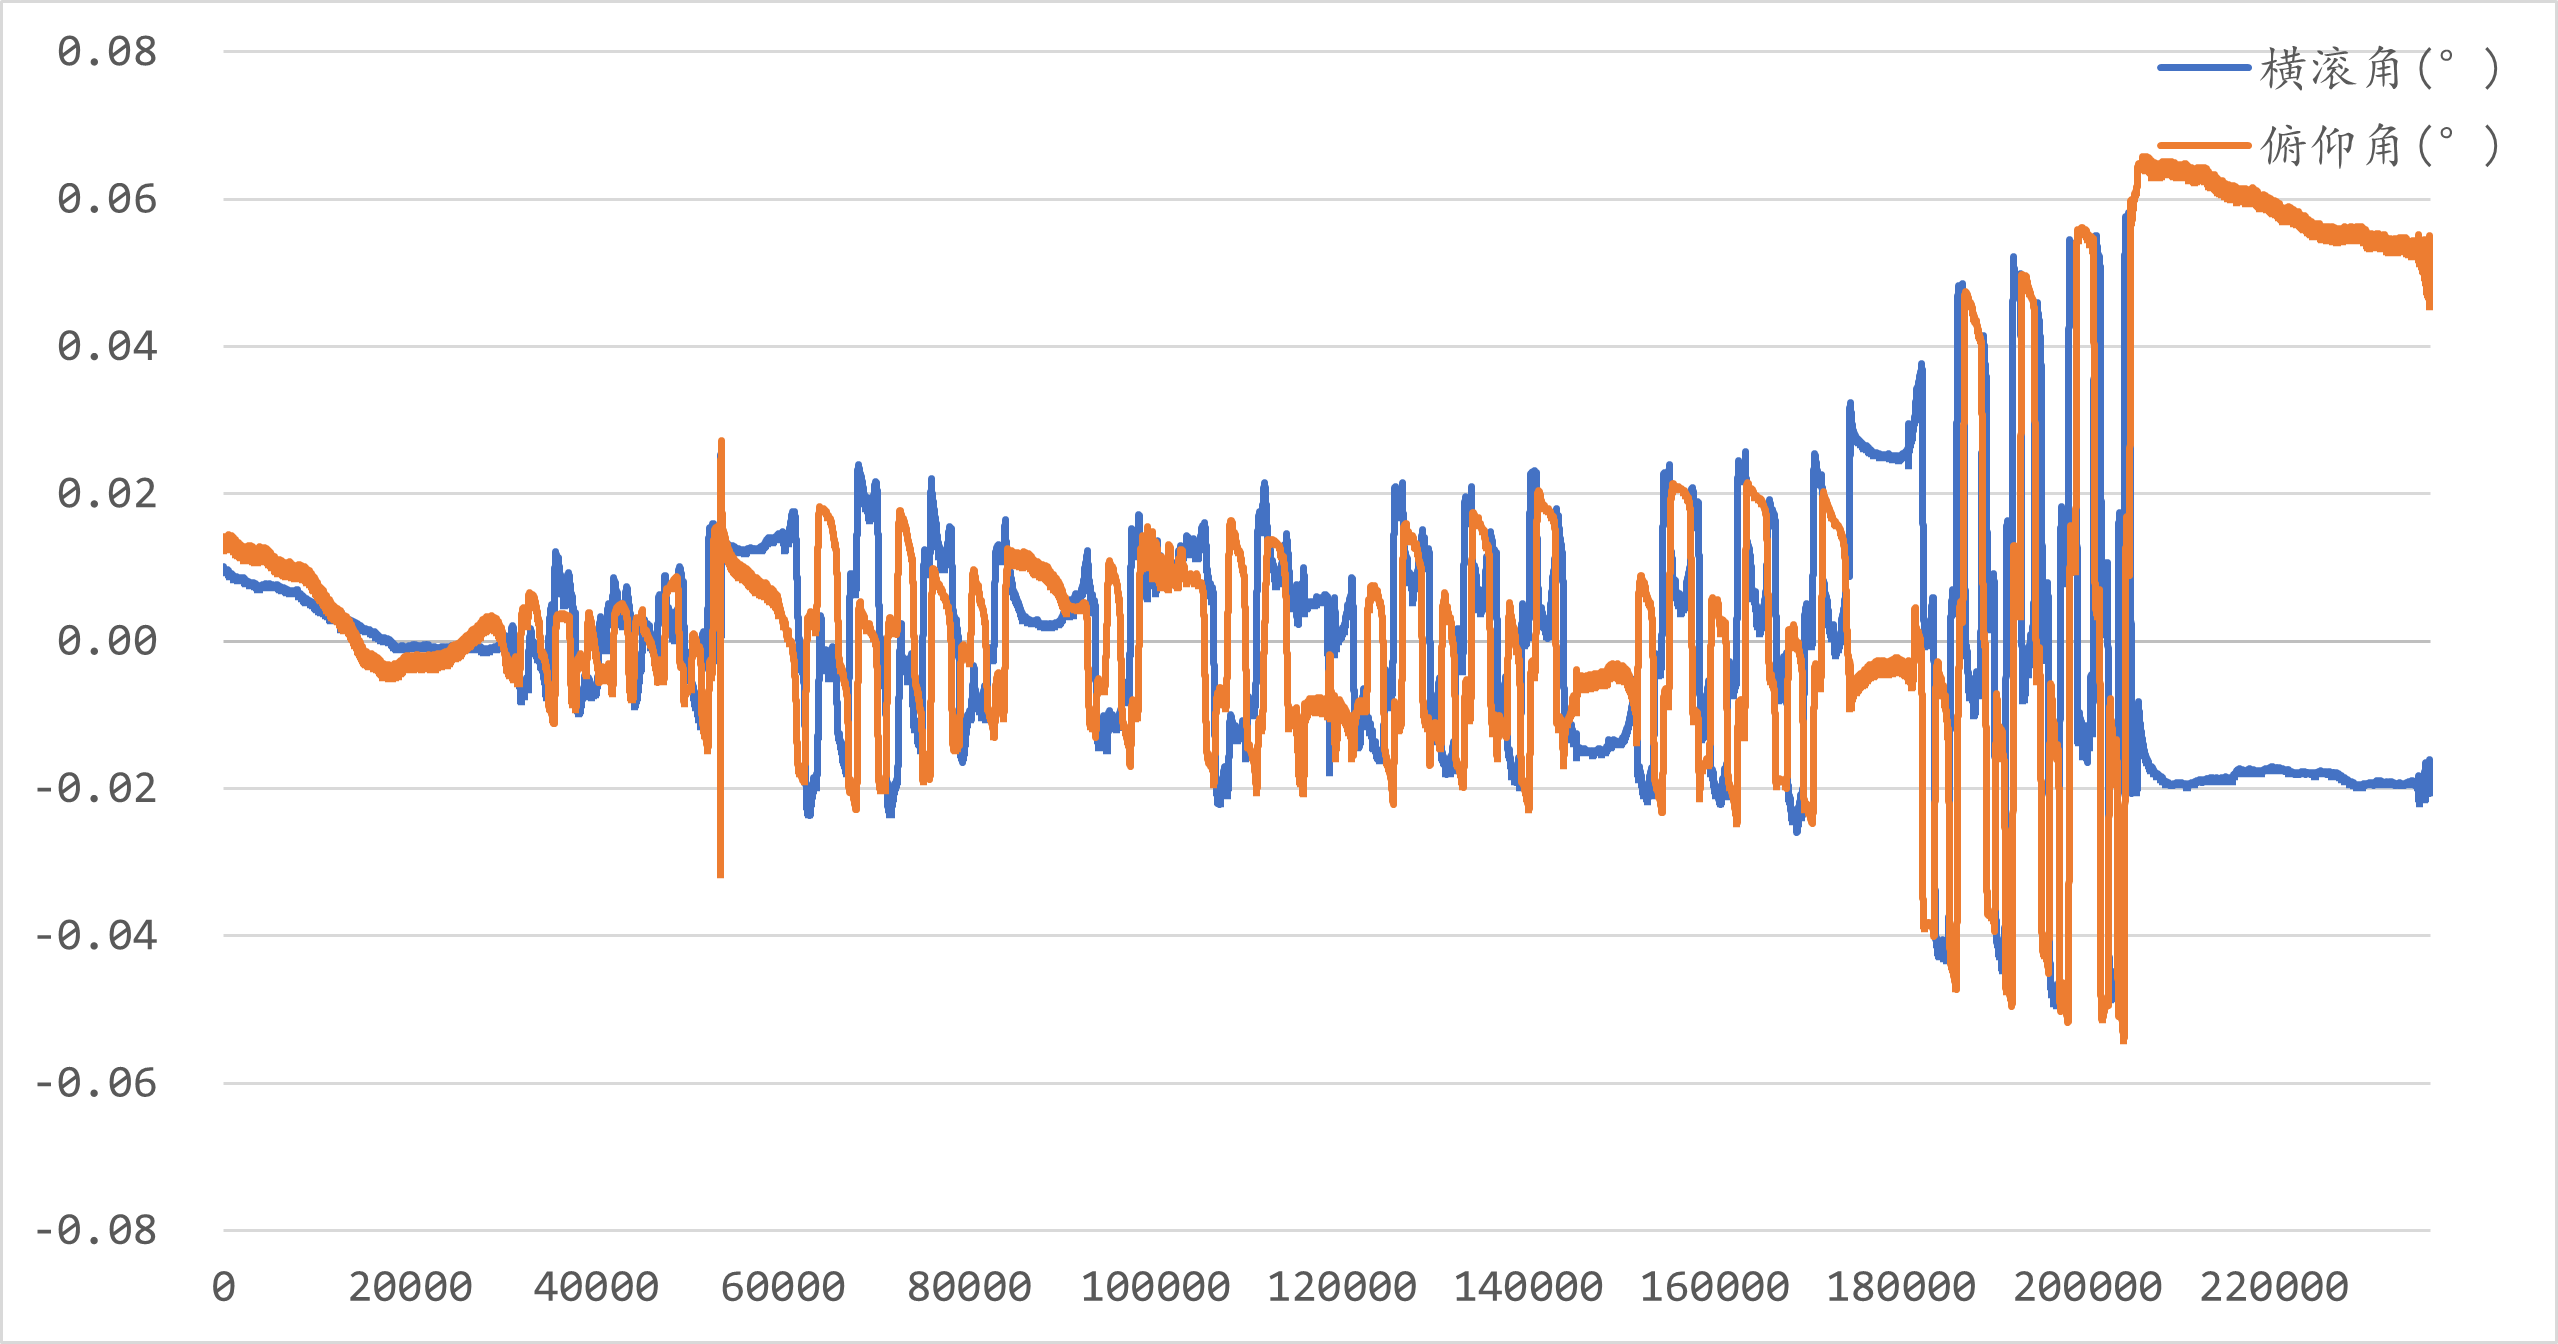
\includegraphics[width=\linewidth]{Figures/DataFigure/灵素修正横滚俯仰角差异.png}
            \caption*{横滚俯仰角差异}
        \end{subfigure}\hfill
        \begin{subfigure}{0.49\textwidth}
            \centering
            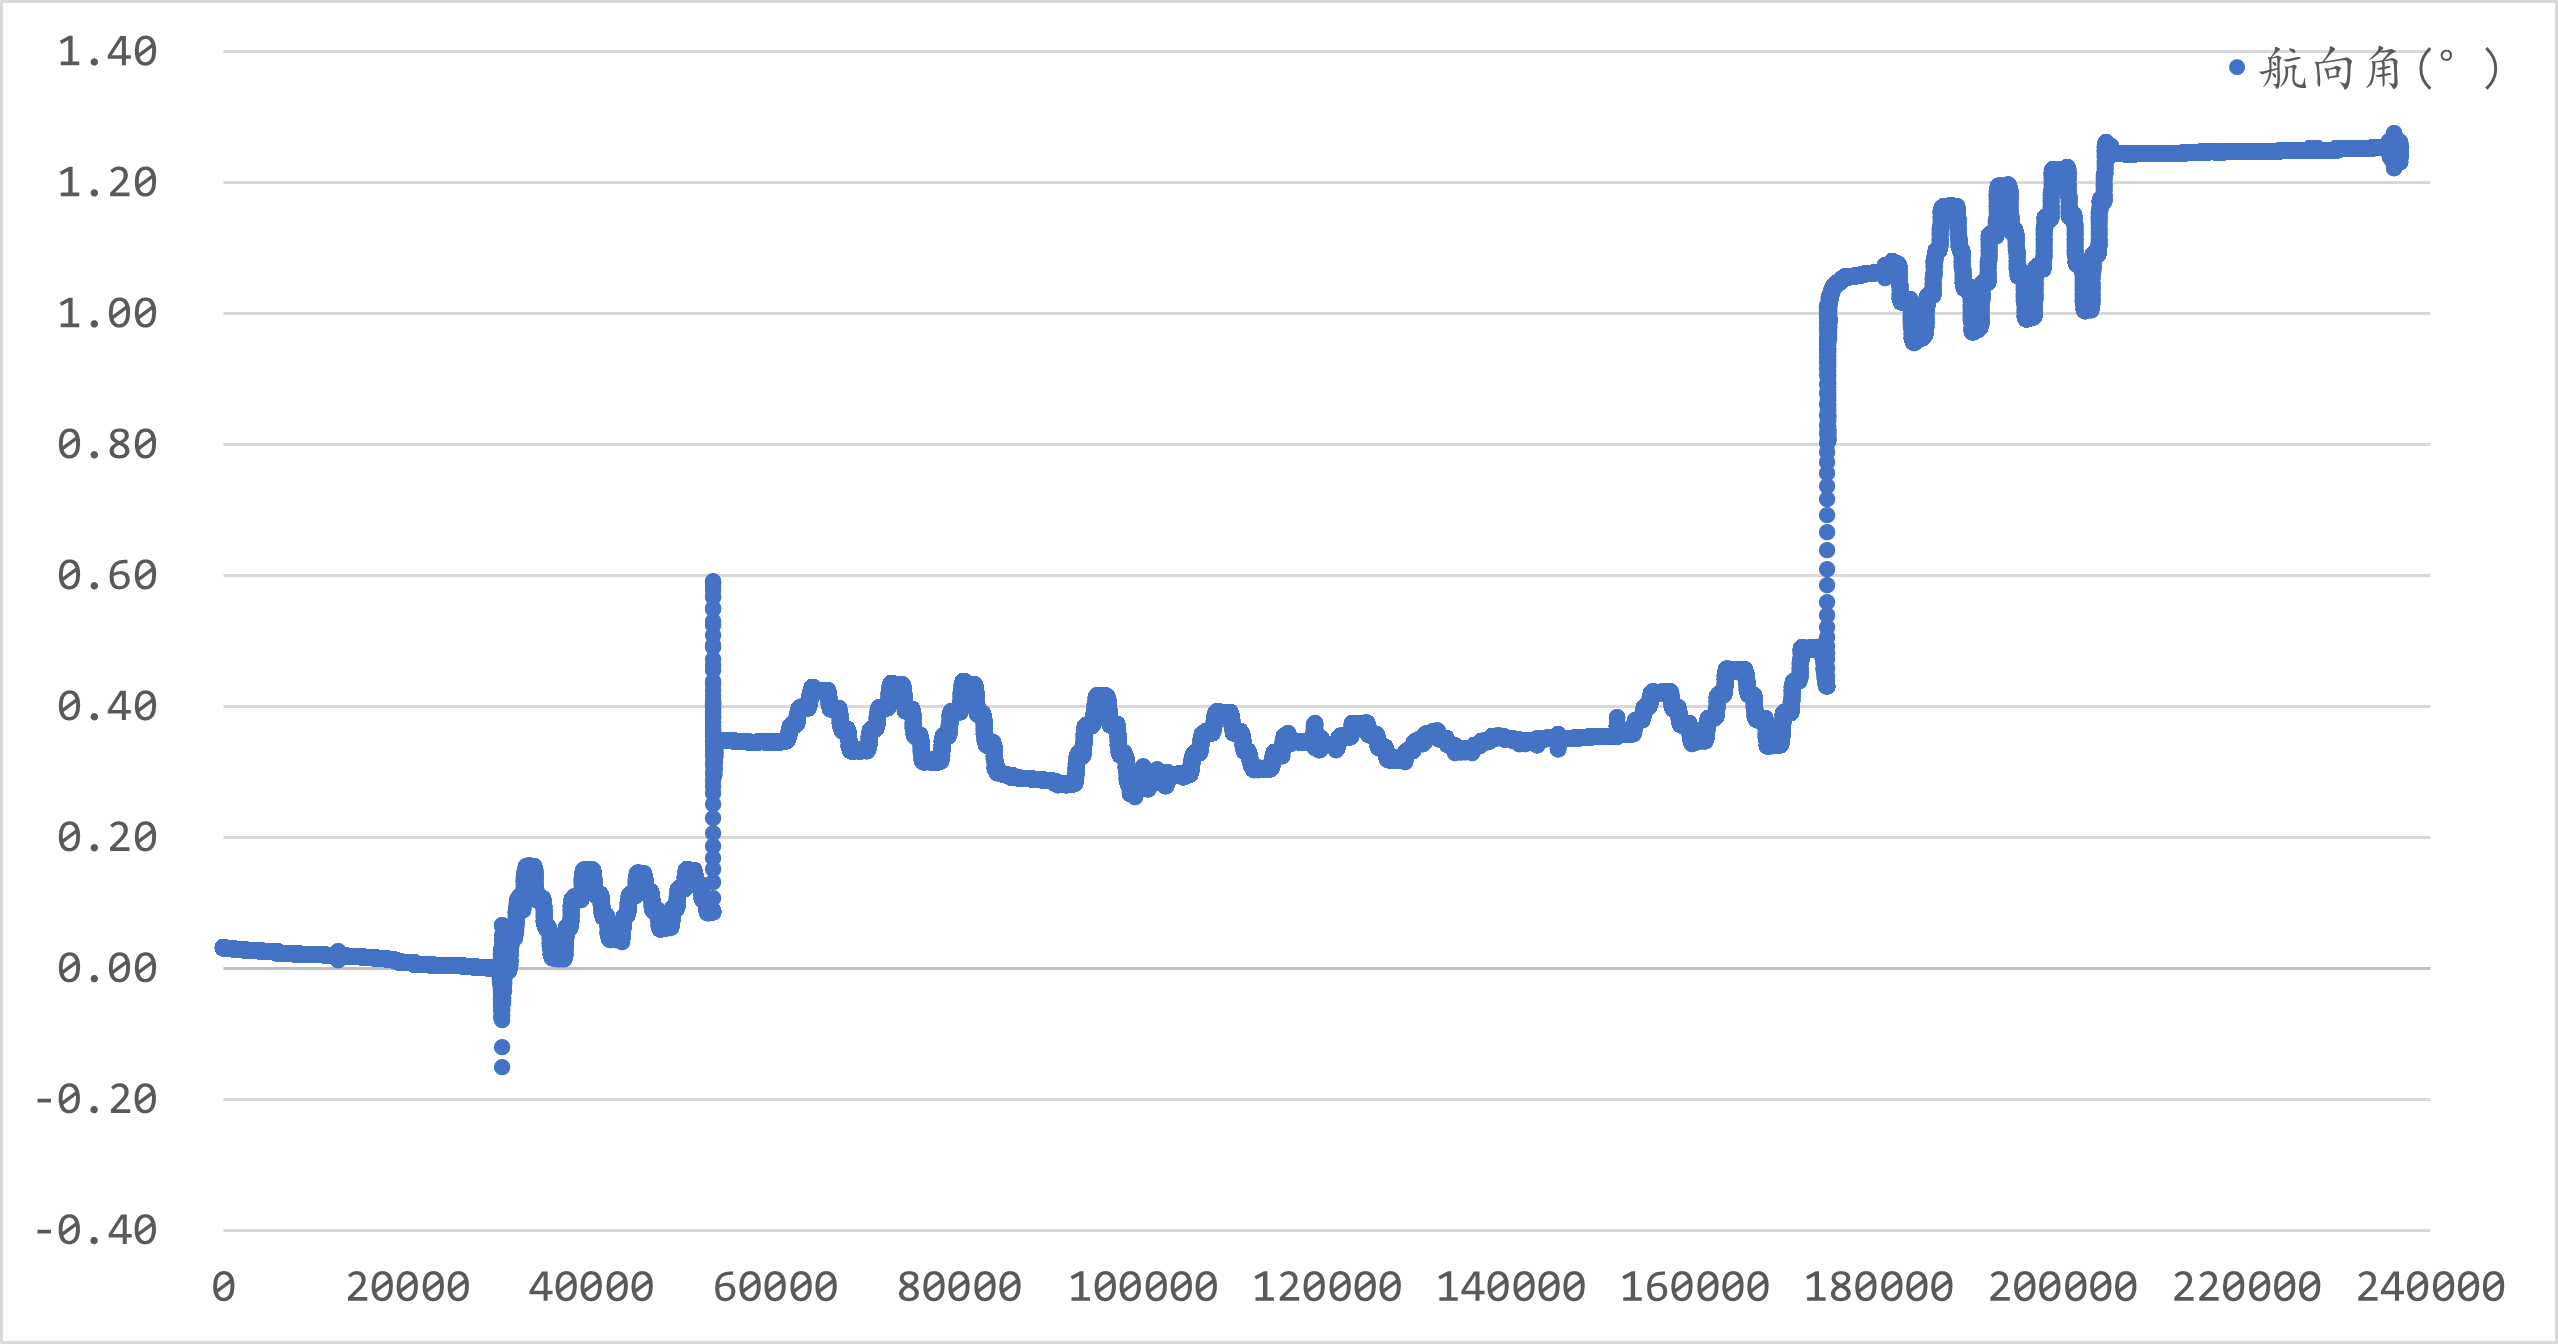
\includegraphics[width=\linewidth]{Figures/DataFigure/灵素修正航向角差异.png}
            \caption*{航向角差异}
        \end{subfigure}
        
        \begin{subfigure}{0.49\textwidth}
            \centering
            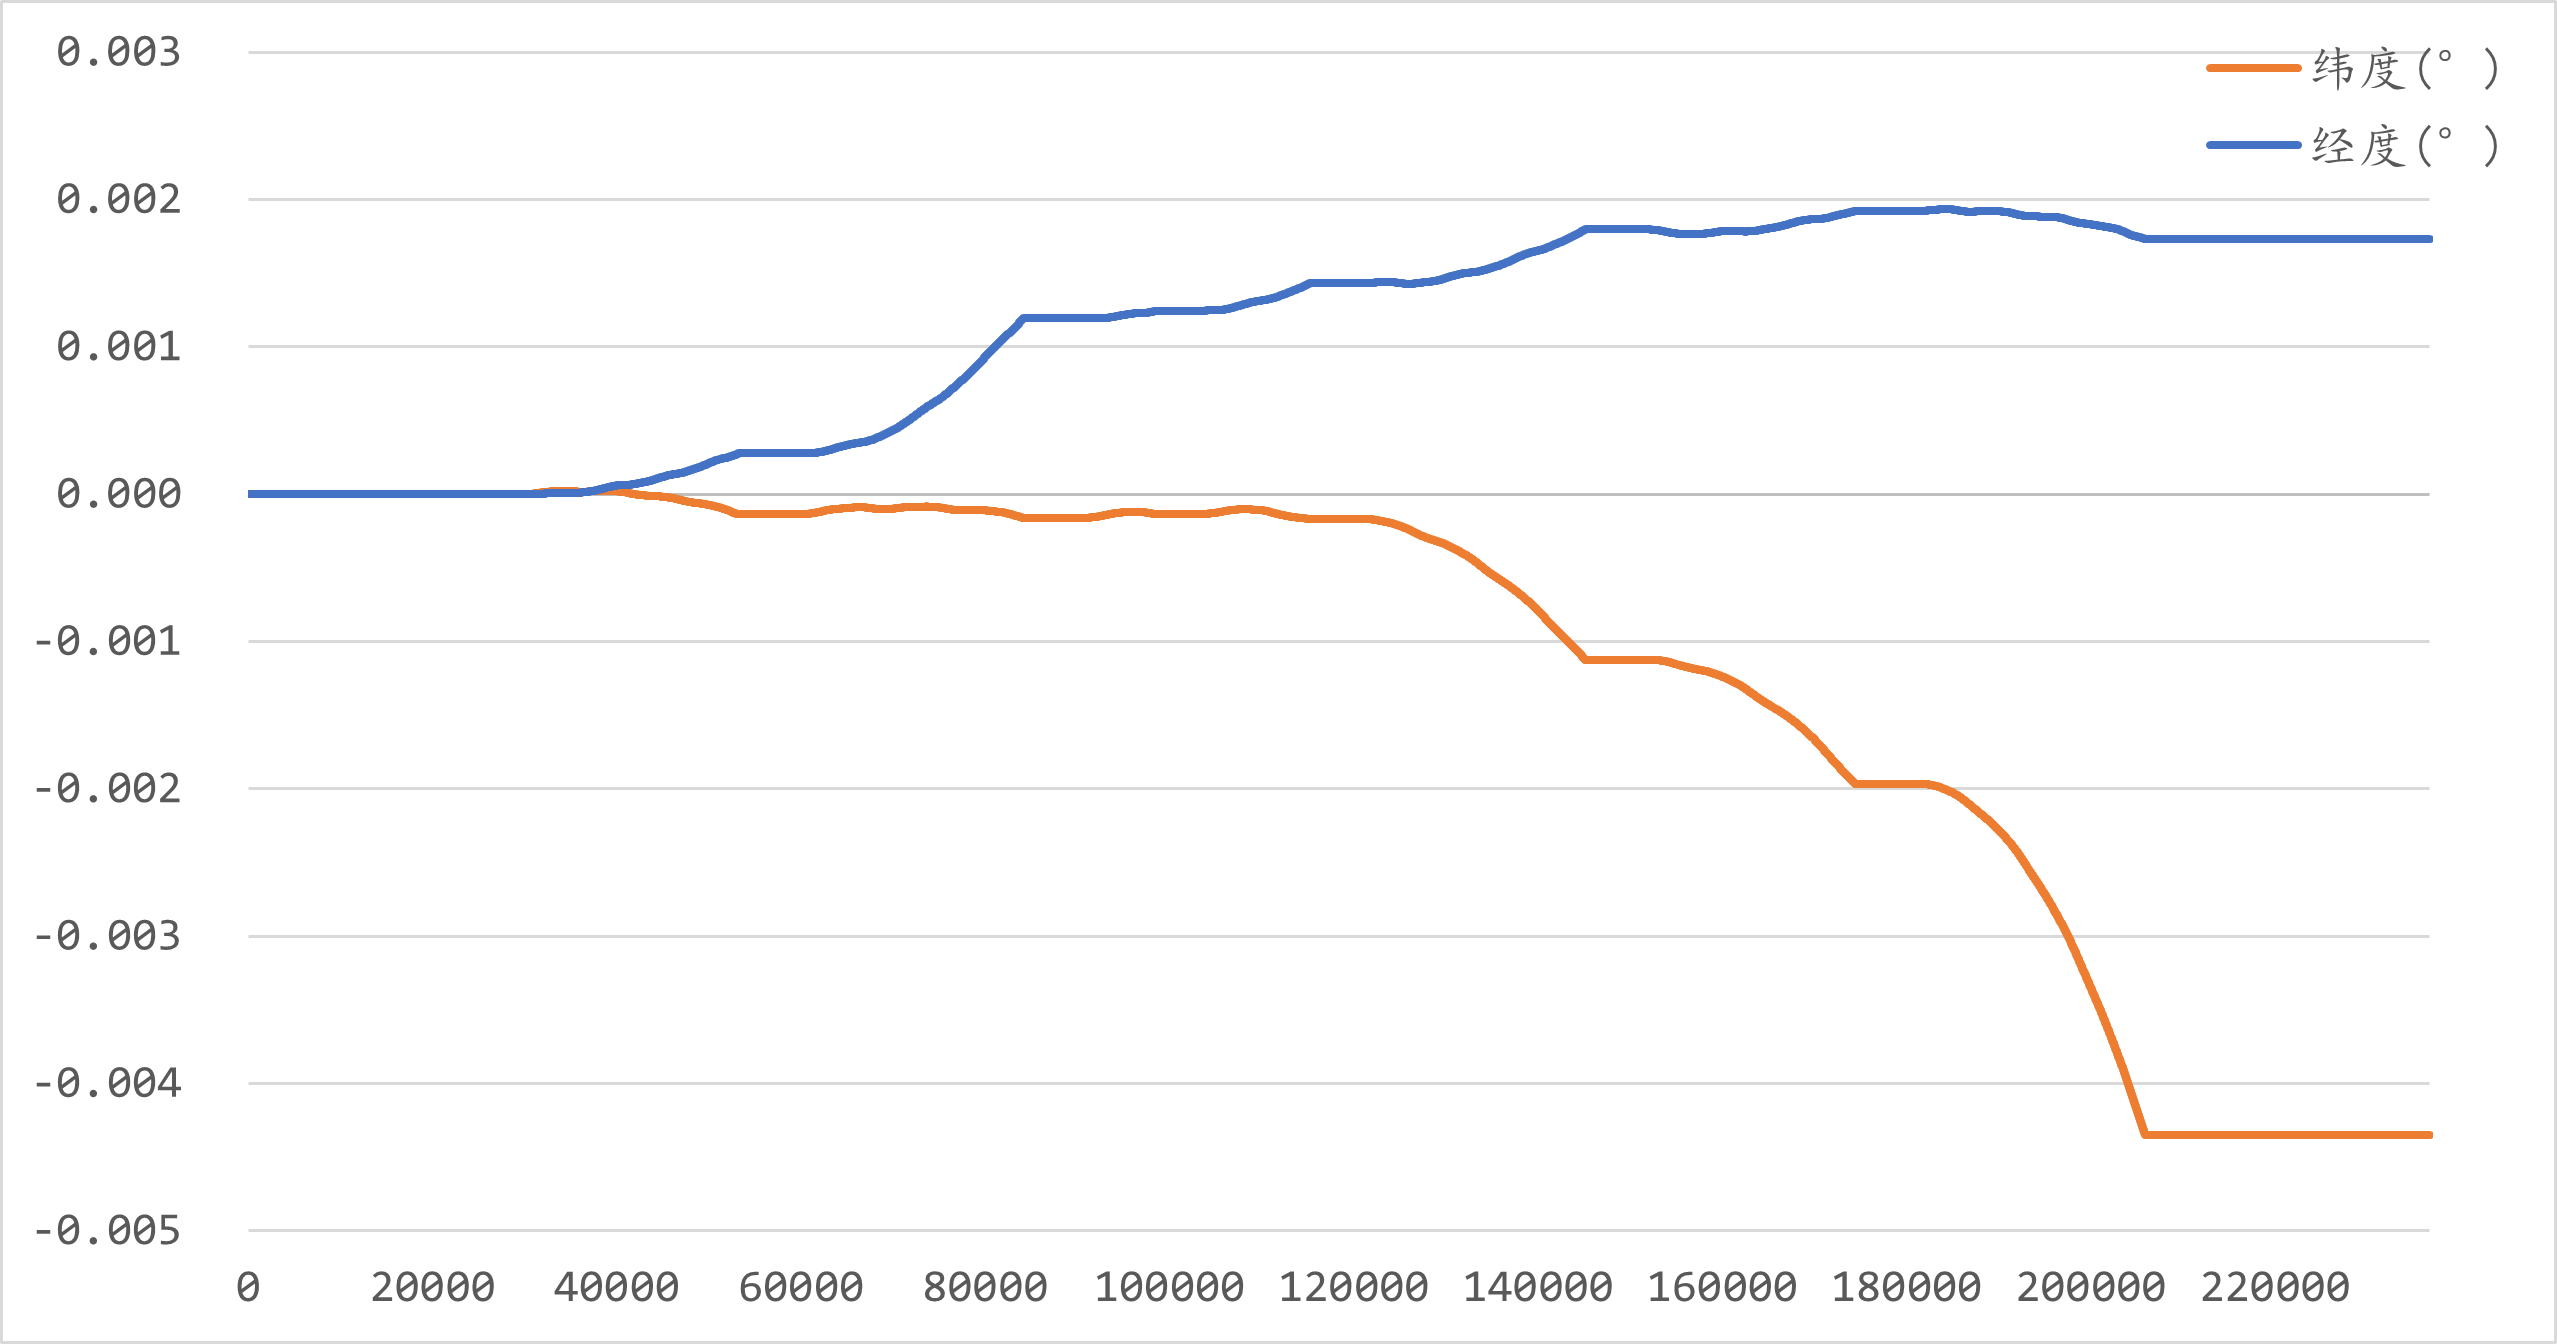
\includegraphics[width=\linewidth]{Figures/DataFigure/灵素修正经纬度差异.png}
            \caption*{经纬度差异}
        \end{subfigure}\hfill
        \begin{subfigure}{0.49\textwidth}
            \centering
            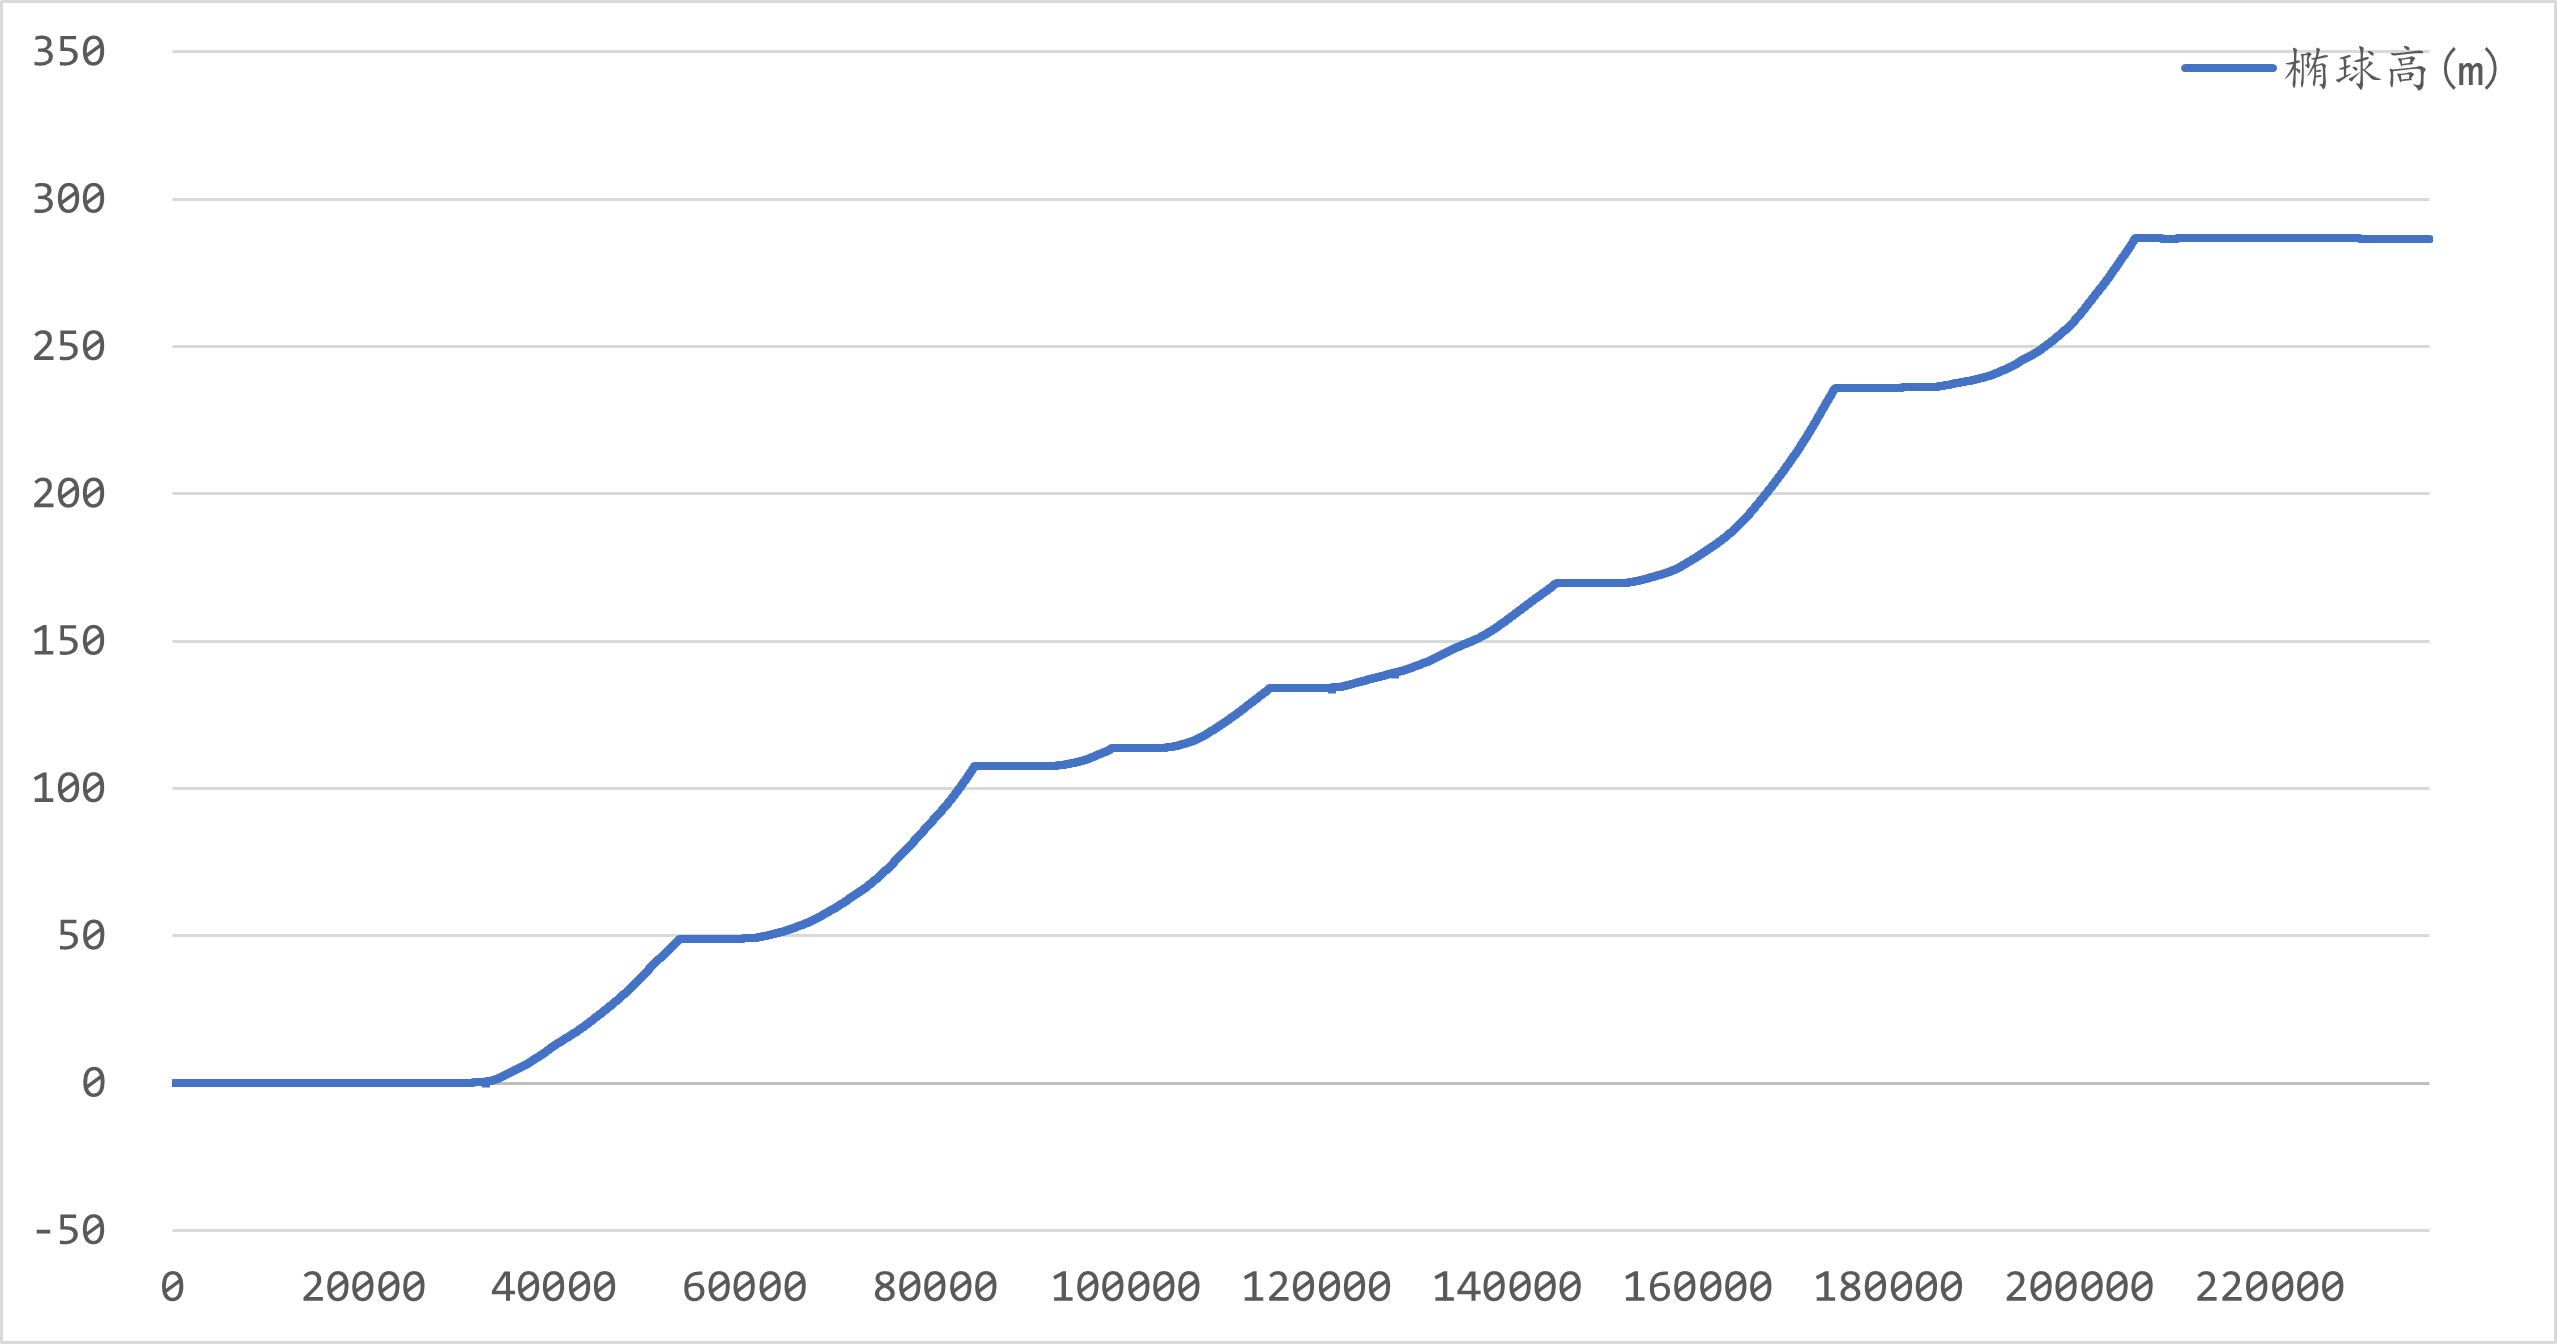
\includegraphics[width=\linewidth]{Figures/DataFigure/灵素修正高程差异.png}
            \caption*{椭球高差异}
        \end{subfigure}

        \begin{subfigure}{0.49\textwidth}
            \centering
            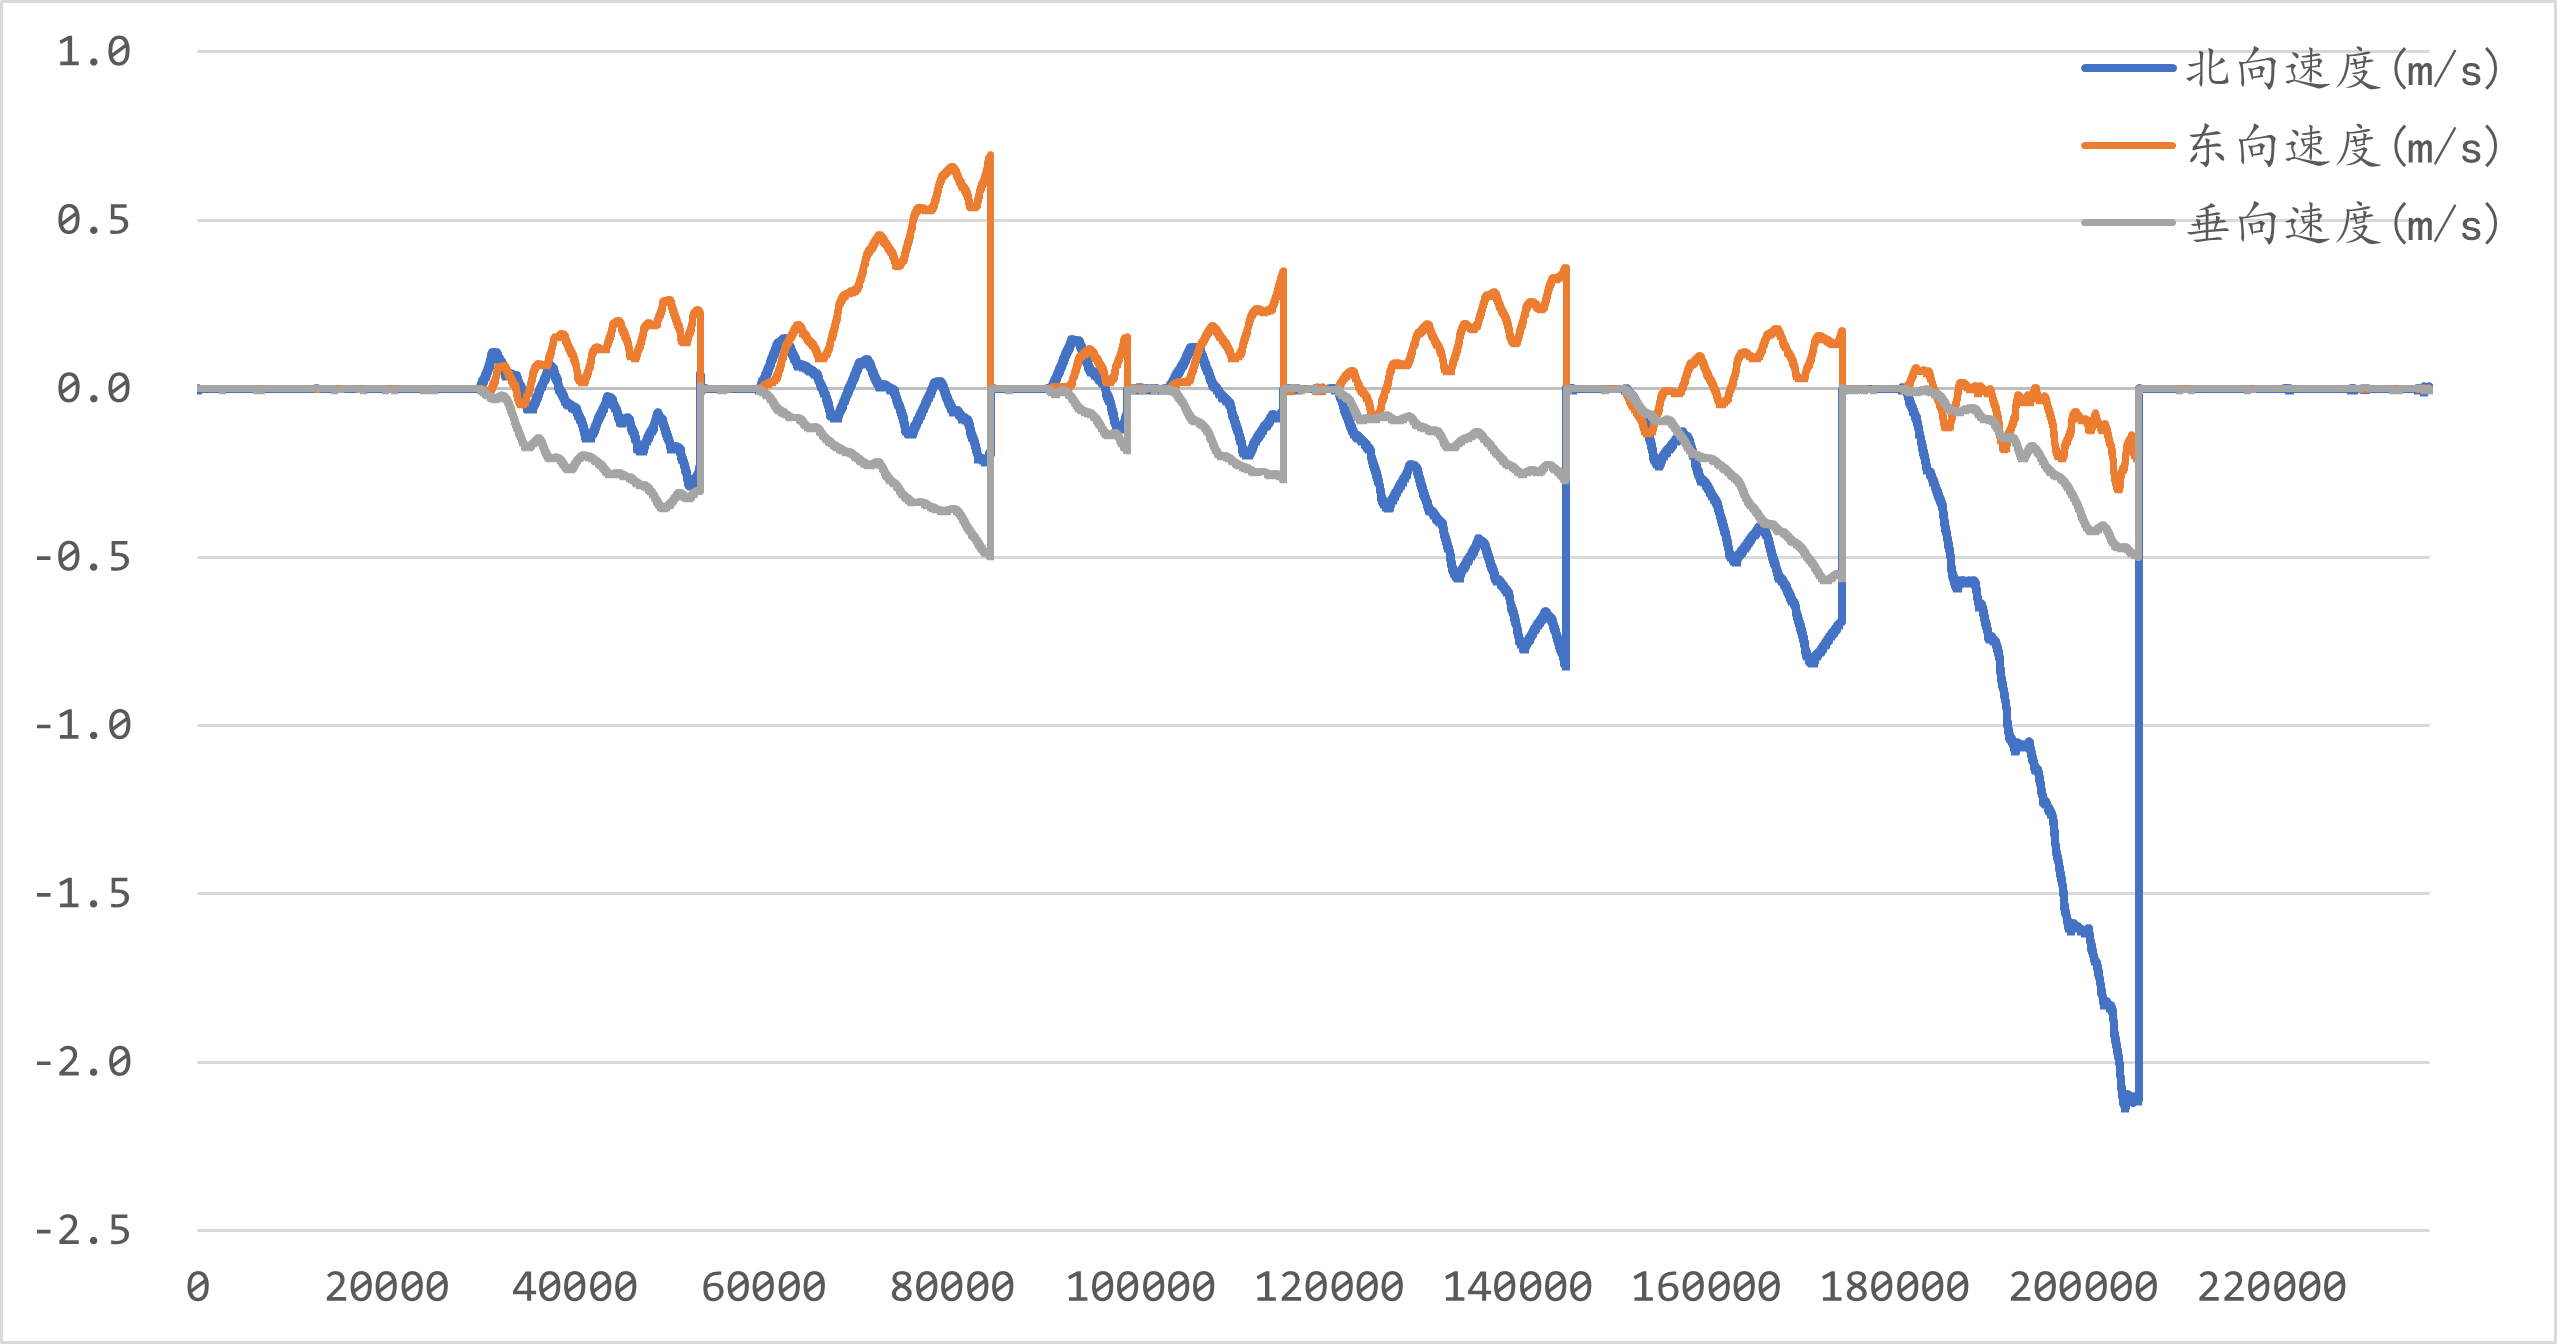
\includegraphics[width=\linewidth]{Figures/DataFigure/灵素修正速度差异.png}
            \caption*{速度差异}
        \end{subfigure}\hfill
        \begin{subfigure}{0.49\textwidth}
            \centering
            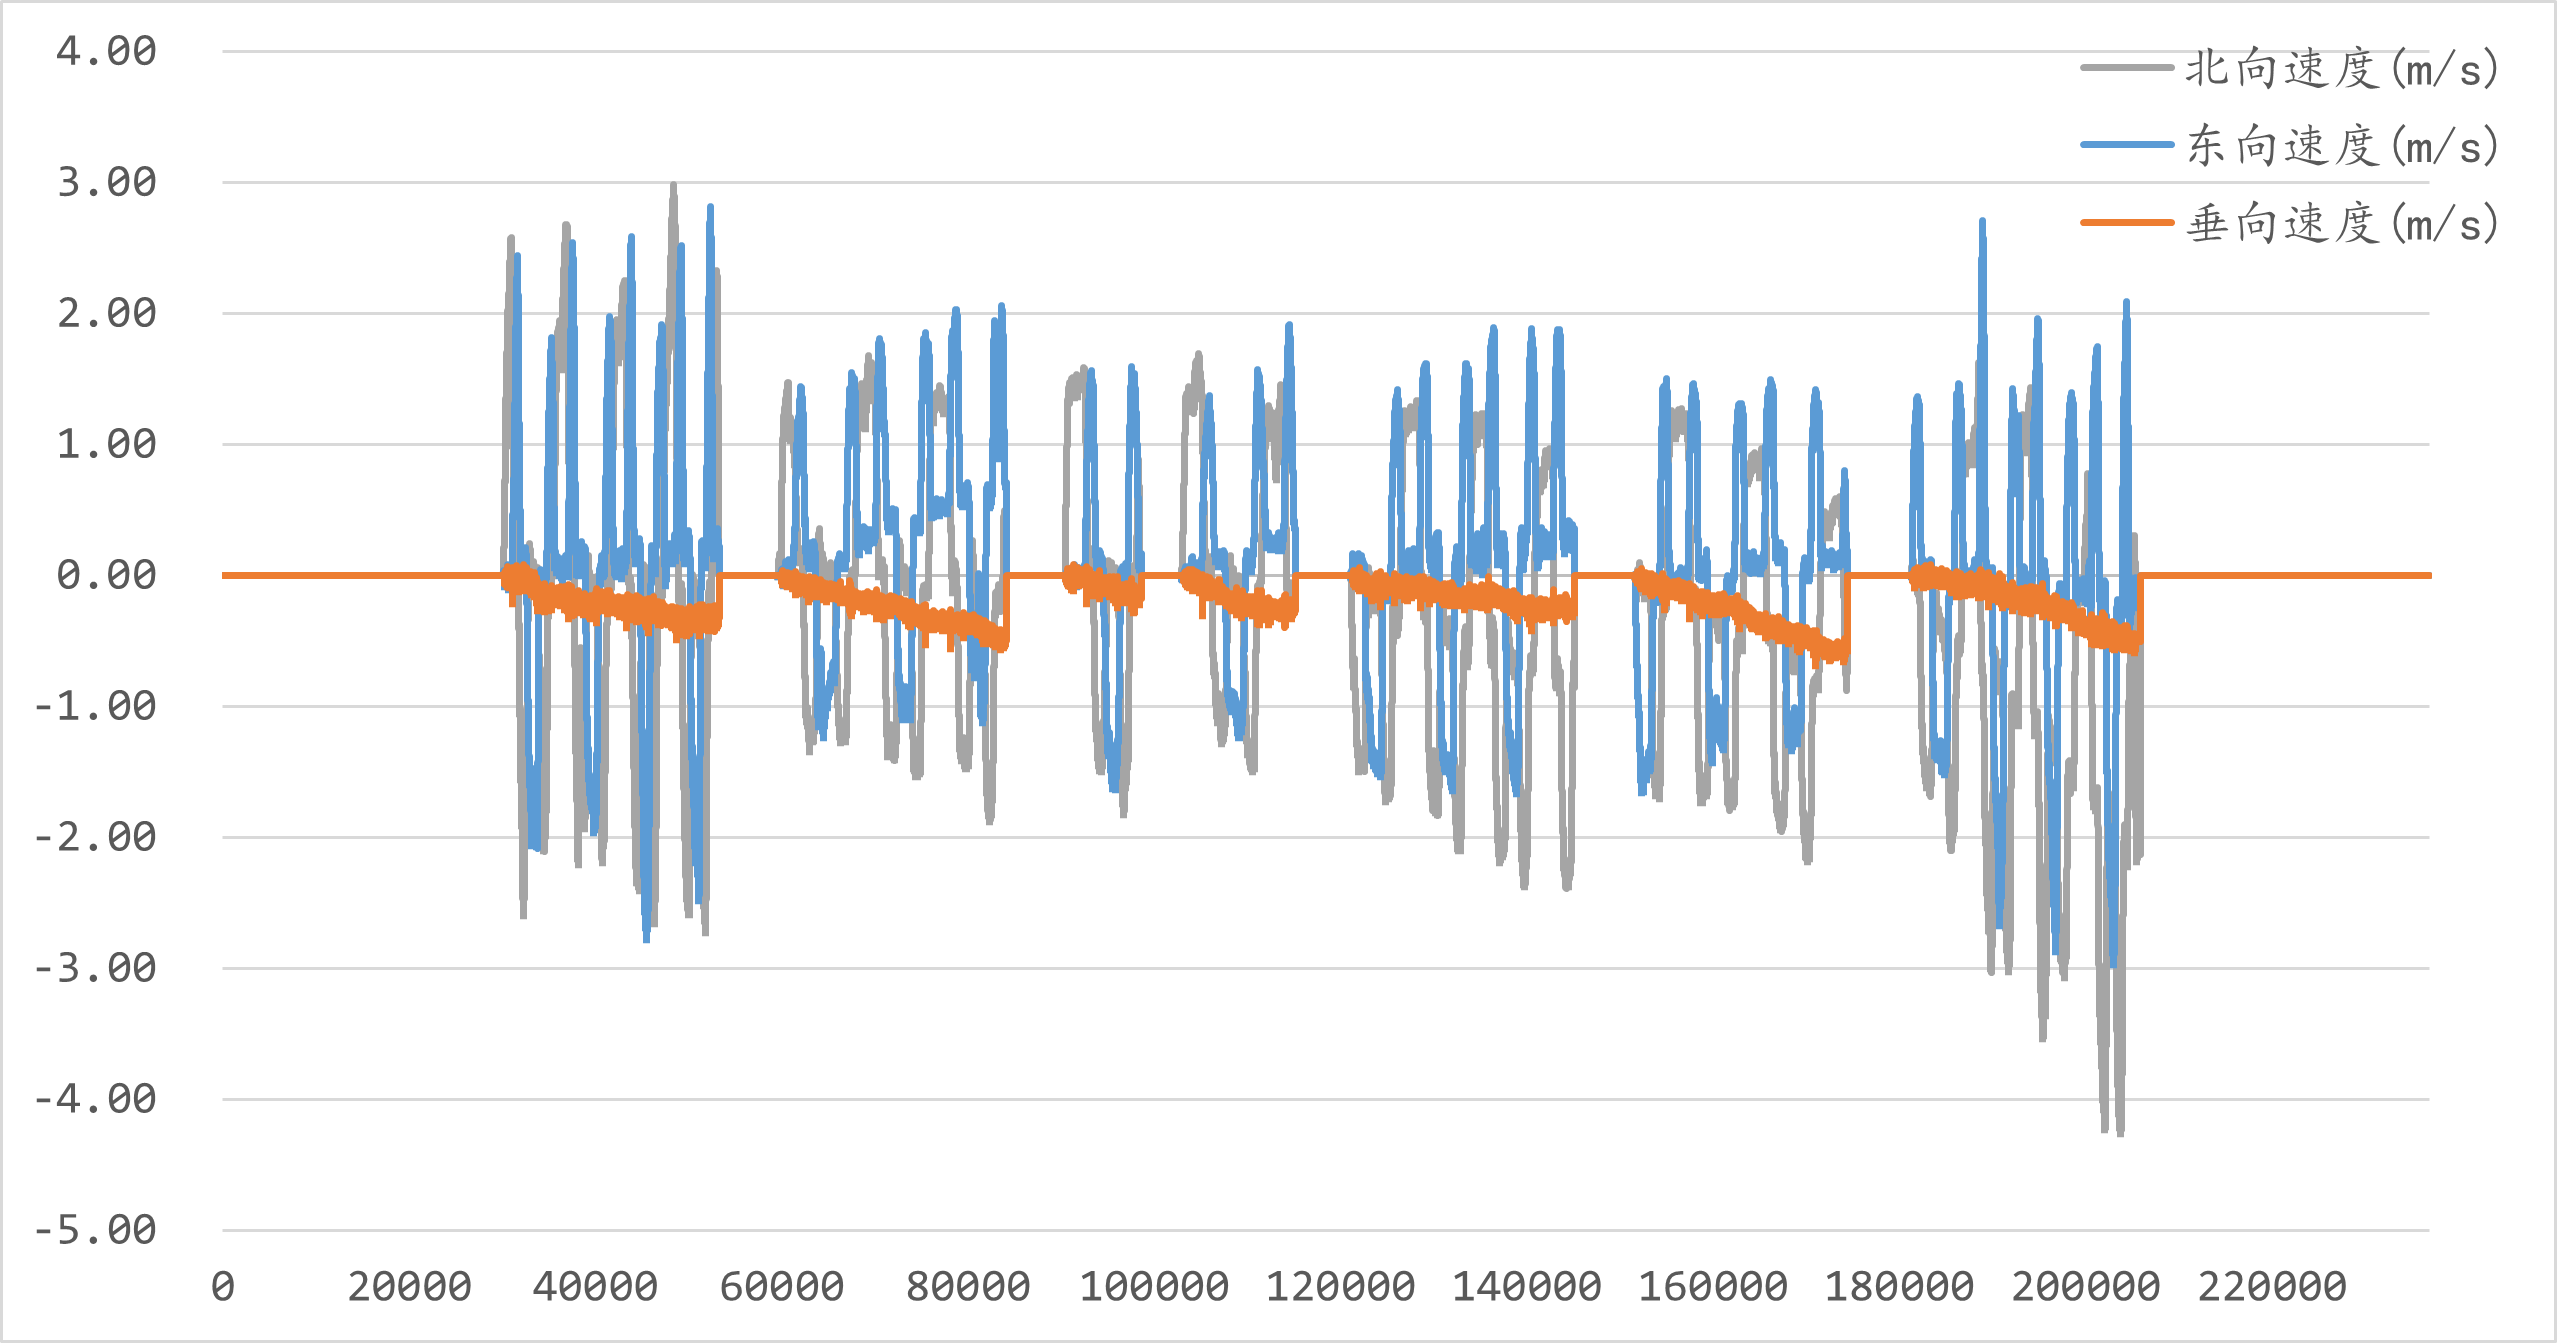
\includegraphics[width=\linewidth]{Figures/DataFigure/灵素修正速度.png}
            \caption*{速度数据}
        \end{subfigure}
    }
    \caption{零速修正数据}
    \label{fig:6.5}
\end{figure}
\noindent 根据速度差异和速度数据的图片来看,很明显中间静止的一分钟对误差起到了抑制作用,让累积的速度误差归零,所以高程曲线会出现阶梯形状.椭球高也从不零速修正的1.4km降到了约300m.可见零速修正对于误差的影响是非常大的.根据\eqref{eq:6.2}式,我们知道静止时如果使用\IMU 的输出数据进行更新,那么短时间内高程误差会随着垂向加速度计误差以二次函数发散,同时由于前一段时间的误差积累,各项初始误差也会比较大,最终导致高程方向迅速发散.而零速修正直接将高程设置为不变,避免了静止时段高程误差的进一步累积.而对于水平方向误差,以北向位置误差为例,有:
\begin{equation}\label{eq:6.3}
    \delta r_N(t) =\delta r_{N,0} + \frac{\sin \omega_s t}{\omega_s} \delta v_{N,0} + R(1 - \cos \omega_s t)\phi_E + \frac{1 - \cos \omega_s t}{\omega_s^2} \delta f_N.
\end{equation}
当$\omega_s t$很小的时候,可以近似为
\begin{equation}\label{eq:6.4}
    \delta r_N(t) =\delta r_{N,0} +\delta v_{N,0} t + \frac{\phi_E g}{2}t^2 + \frac{\delta f_N}{2}t^2.
\end{equation}
可见北向位置误差也是时间的二次函数,所以短时间精致的时候北向位置误差和高程误差发散速度相当,而零速修正则避免了这一点.

\section{问题与思考}

\noindent\textbf{Problem1}.为什么纯惯导的高程误差累积速度比平面快?

在短时间静止时,根据\eqref{eq:6.4}和\eqref{eq:6.2}式,我们发现$\delta r_N$和$\delta h$都是时间的二次函数,而且$\delta h$的二次系数为$\omega_s\delta h_0+\omega_N \delta v_E-\delta f_D/2$,\,$\delta r_N$的二次系数为$(\phi_E g+\delta f_N)/2$,从这一点来说,其实并不一定高程误差累计速度比平面快,因为都是二次函数发散,甚至有可能平面累积更快.例如在本次实验数据中,将初始状态设为$450501.020$s的真实状态,以参考数据为真值,在初始对准的前五分钟不做零速修正,其北向误差和高程误差如下图所示:
\begin{figure}[H]
    \centering
    {
        \captionsetup{textfont={footnotesize,tt}}
        \begin{subfigure}{0.49\textwidth}
            \centering
            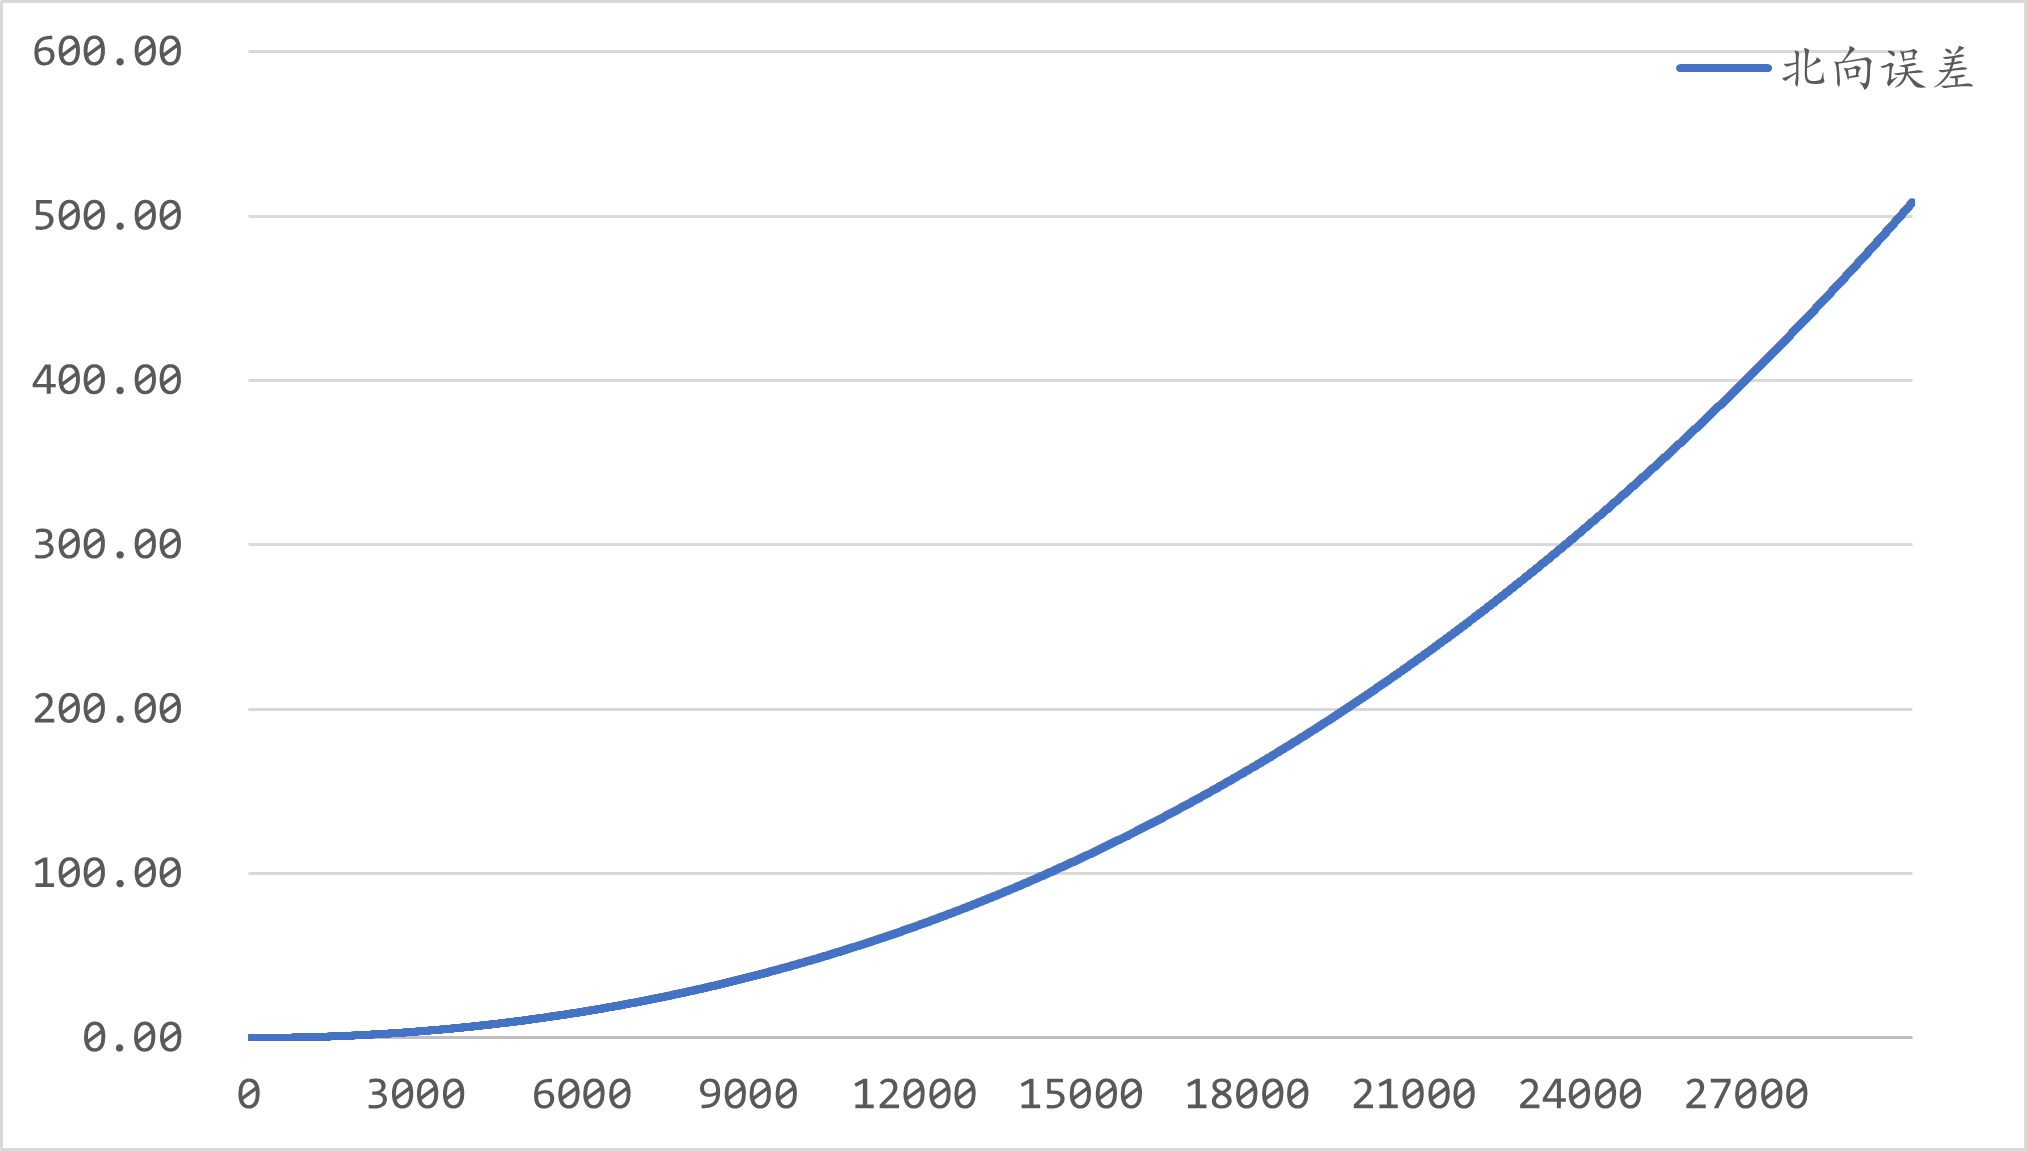
\includegraphics[width=\linewidth]{Figures/DataFigure/未零速修正北向误差.png}
        \end{subfigure}\hfill
        \begin{subfigure}{0.49\textwidth}
            \centering
            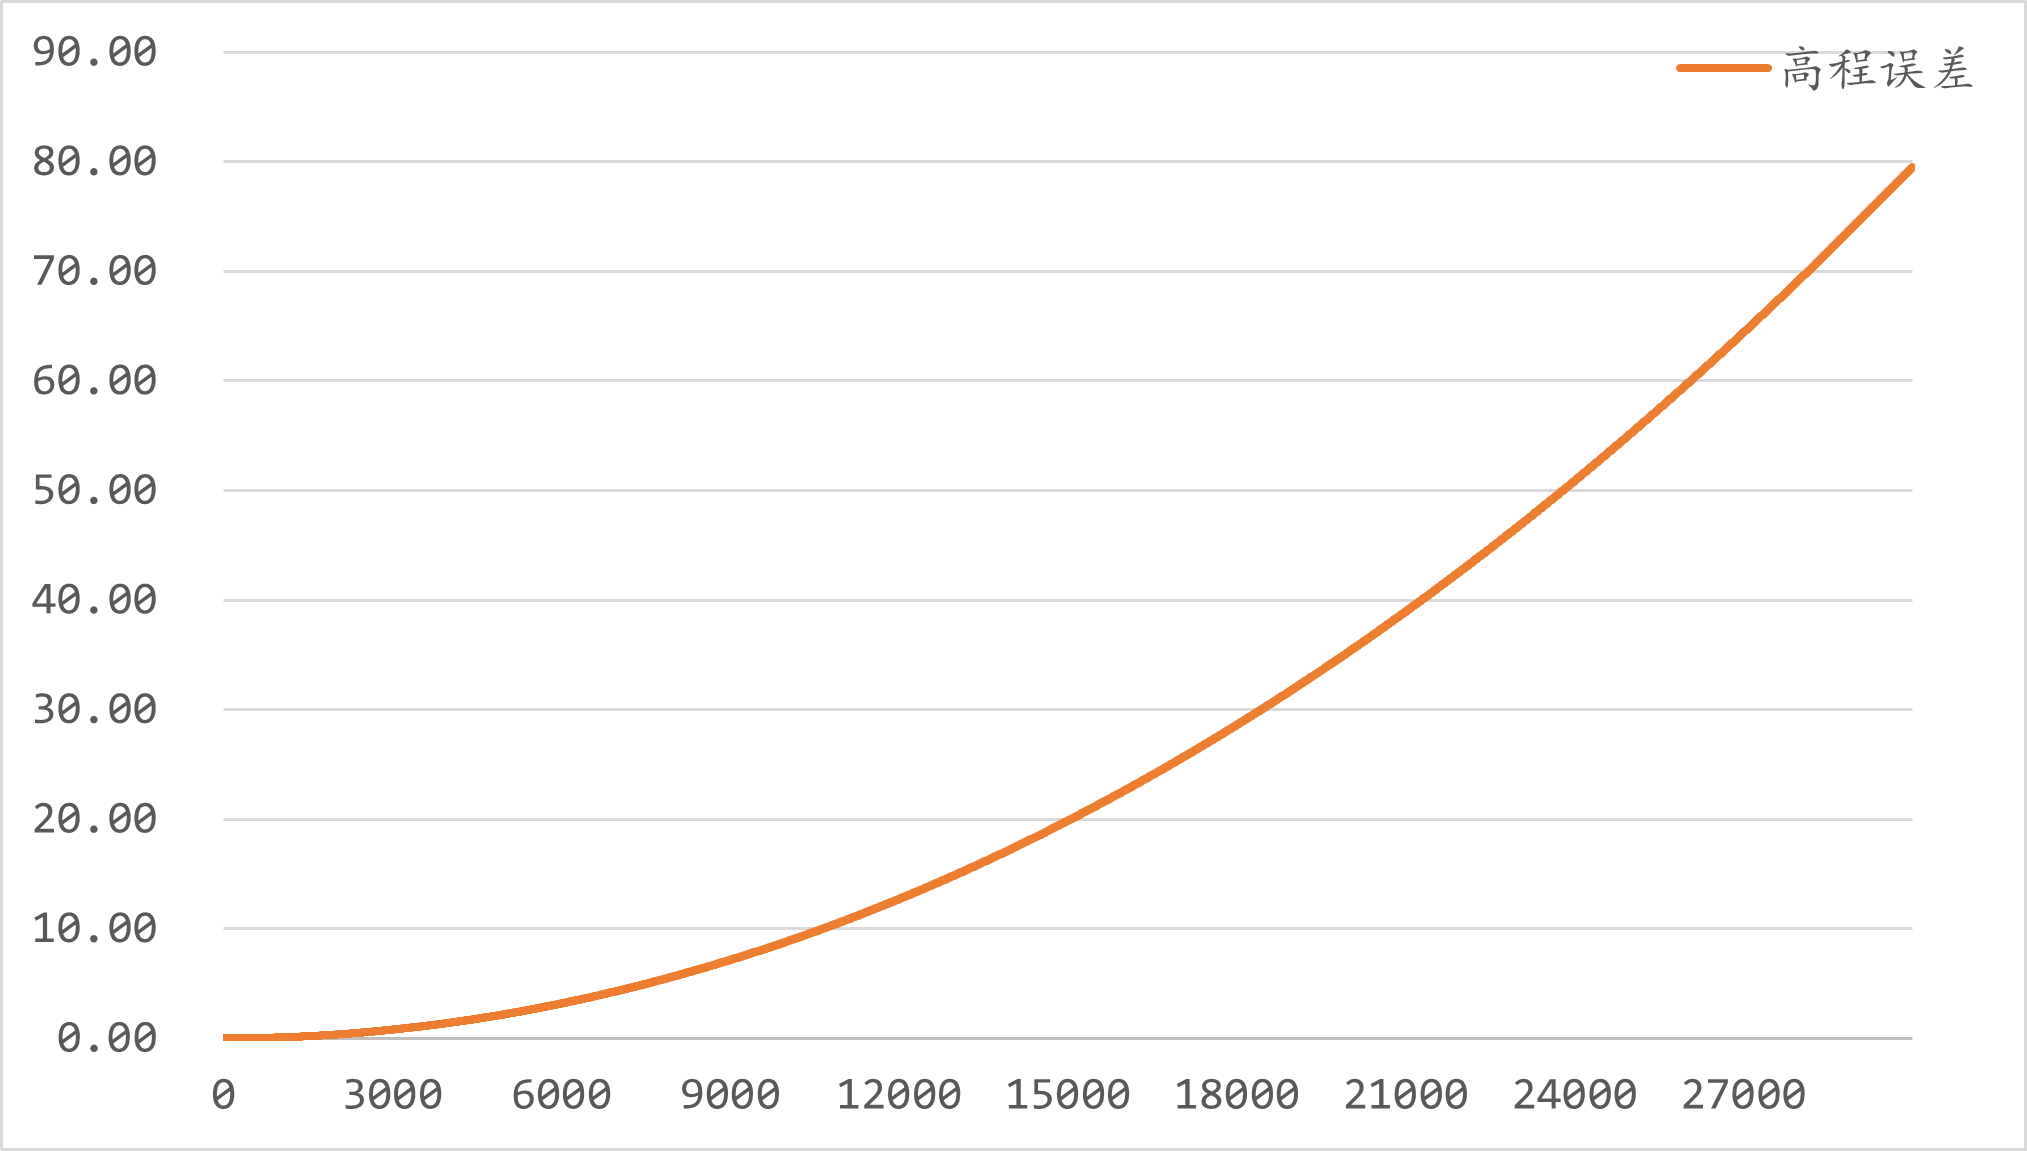
\includegraphics[width=\linewidth]{Figures/DataFigure/未零速修正高程误差.png}
        \end{subfigure}
    }
    \caption{前五分钟未零速修正误差}
    \label{fig:7.1}
\end{figure}
\noindent 显然此时平面误差累积更快.但是总体都符合二次函数的形状.如果长时间静止,根据\eqref{eq:6.1}式和\eqref{eq:6.3}式,高程误差是指数发散而北向位置误差是三角函数,所以这时高程误差发散的更快.

\noindent\textbf{Problem2}.为什么用示例数据对比的差异很小而小推车的纯惯导误差却大很多?

\noindent 纯惯导的定位解算基于积分,这样一来,之前的定位误差也会被带到下一个时刻的误差中,所以纯惯导定位误差也和初始状态的误差有关,如果\IMU 本身的精度不高,如零偏大,就会导致误差随着时间累积迅速发散.所以为了避免误差过快的积累,一方面我们需要进行初始对准提高初始状态的精度,另一方面要进行零速修正等约束.而示例数据使用了\textsf{GNSS}和\textsf{INS}的送组合进行计算,用\textsf{GNSS}观测值不断修正\IMU 的误差,得到定位结果的最佳估计值,所以误差比纯惯导要小得多,但是很明显如果在\textsf{GNSS}信号遮挡严重的情况下,松组合的可靠性也可能较差.

总的来说,本次实验是惯性导航课程的一次综合实验.在运用所有所学内容的同时让我们进一步体会纯惯导解算的工作流程,即如何进行姿态,速度和位置更新.也让我们直观地了解到纯惯导的误差累积情况.具体到个人来说,对惯性导航课程的整个知识体系有一个连贯的理解,不再把每一章的内容分开看待.虽然由于时间原因,算法原理文档只写到了四元数部分,但是在编程和误差分析的过程中,对整个算法有了一个更清晰的认识.对于编程来说也是一次很好的锻炼,如何写出一个可读性强效率高的代码十分值得琢磨,例如矩阵向量类的设计就花费了我不少时间.在最后的分析过程中,我也发现很多地方都可以前后照应,例如在初始对准的学习中,我们知道北向位置误差是随时间的三次函数,即
\[
    \delta r_N =\delta r_{N,0} +\delta v_{N,0}t + \frac{1}{2}(g\delta \theta_0 + b_{aN})t^2 + \frac{1}{6}gb_{gE}t^3,
\]
在静基座惯导误差分析的过程中,我们知道北向位置误差可以写为\eqref{eq:6.3}式,在短时间内,展开到三阶项,即
\[
    \delta r_N =\delta r_{N,0} +\delta v_{N,0}t + \frac{1}{2}(g\phi_E +\delta f_N)t^2 - \frac{1}{6}g\frac{\delta v_{N,0}}{R} t^3,
\]
在高程为$0$的情况下,有$v_{N,0}/R=-\omega_{E,0}$,所以这两个误差公式形式其实是完全一致的.

\appendix
\section{自编程序与报告代码}
\noindent 该程序需要在\texttt{.NET7}环境下运行并且确保已安装\textsf{Excel}. \texttt{Github}\hspace{0mm}仓库链接为\url{https://github.com/Eliaul/INS}.




\end{document}